%This is a very basic  BE PROJECT PRELIMINARY template.

%#############################################
%#########Author :  PROJECT###########
%#########COMPUTER ENGINEERING############


\documentclass[oneside,a4paper,12pt]{report}
%\usepackage{showframe}
%\hoffset = 8.9436619718309859154929577464789pt
%\voffset = 13.028169014084507042253521126761pt

\fancypagestyle{plain}{%
  \fancyhf{}
  \fancyfoot[CE]{College_Name, Department of Computer Engineering 2015}
  \fancyfoot[RE]{\thepage}
}
\pagestyle{fancy}
\fancyhead{}
\renewcommand{\headrulewidth}{0pt}
\footskip = 0.625in
\cfoot{}
\rfoot{}

\usepackage{tikz}
\usetikzlibrary{arrows,shapes,snakes,automata,backgrounds,petri}
\usepackage{ltablex}

%\usepackage[nottoc,notlot,notlof,numbib]{tocbibind}
\usepackage[titletoc]{appendix}
\usepackage{titletoc}
\renewcommand{\appendixname}{Annexure}
\renewcommand{\bibname}{References}

\setcounter{secnumdepth}{5}

\usepackage{float}
\usepackage{subcaption}
\usepackage{multirow}

\usepackage[ruled]{algorithm2e}

\usepackage{amssymb}
\usepackage{tikz}
\usepackage{pdfpages}

\usepackage{caption}
\usepackage{subcaption}
\usepackage{multirow}
\usepackage{multicol}


\usepackage{xcolor}

%\definecolor{offwhite}{RGB}{255,255,243}
%\pagecolor{offwhite}


\usepackage[authoryear]{natbib}

\usepackage[colorlinks=true, linkcolor=black, citecolor=blue]{hyperref}
\usepackage{listings}

\usetikzlibrary{arrows.meta, chains, shapes.geometric}

\tikzset{FlowChart/.style = {% for distinguish from other tikz sets used in your document
     base/.style = {ellipse, draw,
                    minimum width=3cm, minimum height=1cm, align=center,
                    text width =\pgfkeysvalueof{/pgf/minimum width}-2*\pgfkeysvalueof{/pgf/inner xsep},
                    on chain, join=by arrow},
startstop/.style = {base, fill=red!30, rounded corners},
       io/.style = {trapezium, trapezium left angle=70, trapezium right angle=110,
                    trapezium stretches body,
                    draw=black, fill=blue!30,
                    minimum width=1cm, minimum height=1cm, align=center,
                    on chain, join=by arrow},
input/.style    =  {coordinate,node distance=2em},
   process/.style = {base, fill=orange!30},
  decision/.style = {diamond, aspect=1.2, draw, fill=green!30,
                     minimum width=3cm, minimum height=1cm, align=center,
                     on chain, join=by arrow},
     arrow/.style = {thick,-Stealth}}
        }

\usepackage{tikz}
\usetikzlibrary{arrows.meta,chains}

\begin{document}
\setlength{\parindent}{0mm}
\begin{center}
% \vspace*{1\baselineskip}
{\bfseries A  PROJECT REPORT ON \\}
 \vspace*{2\baselineskip}
{\bfseries \fontsize{16}{12} \selectfont Astronomical Image colorization and super-resolution using GANs \\ \vspace*{2\baselineskip}}
{\fontsize{12}{12} \selectfont SUBMITTED TOWARDS THE
 \\PARTIAL FULFILMENT OF THE REQUIREMENTS OF \\

\vspace*{2\baselineskip}}
{\bfseries \fontsize{14}{12} \selectfont BACHELOR OF ENGINEERING (Computer
Engineering) \\
\vspace*{1\baselineskip}}
{\bfseries \fontsize{14}{12} \selectfont BY \\
\vspace*{1\baselineskip}}
Shreyas Kalvankar  \hspace{25 mm} Exam No: B150134261 \\
Hrushikesh Pandit \hspace{25 mm} Exam No: B150134296  \\
Pranav Parwate \hspace{30 mm} Exam No: B150134299 \\
Atharva Patil \hspace{34 mm} Exam No: B150134303\\
\vspace*{2\baselineskip}
{\bfseries \fontsize{14}{12} \selectfont Under The Guidance of \\
\vspace*{2\baselineskip}}
Prof. Dr. S.M. Kamalapur\\

\includegraphics[width=100pt]{collegelogo.png} \\
{\bfseries \fontsize{14}{12} \selectfont Department of Computer Engineering \\
K. K. Wagh Institute of Engineering Education \& Research \\
Hirabai Haridas Vidyanagari, Amrutdham, Panchavati, Nashik-422003 \\
Savitribai Phule Pune University\\
A. Y. 2020-21 Sem I
}
\end{center}

\newpage



\begin{figure}[ht]
\centering

\includegraphics[width=100pt]{collegelogo.png}
\end{figure}


{\bfseries \fontsize{14}{12} \selectfont \centerline{K. K. Wagh Institute of Engineering Education and Research}
\centerline{Department of Computer Engineering}
\vspace*{3\baselineskip}}


{\bfseries \fontsize{16}{12} \selectfont \centerline{CERTIFICATE}
\vspace*{3\baselineskip}}

\centerline{This is to certify that the Project Titled}
\vspace*{1\baselineskip}


{\bfseries \fontsize{14}{12} \selectfont \centerline{Astronomical Image colorization and super-resolution using GANs}
\vspace*{1\baselineskip}}

\centerline{Submitted by}
\vspace*{1\baselineskip}
\centerline{Shreyas Kalvankar  \hspace{25 mm} Exam No: B150134261}
\centerline{Hrushikesh Pandit \hspace{25 mm} Exam No: B150134296 }
\centerline{Pranav Parwate \hspace{30 mm} Exam No: B150134299}
\centerline{Atharva Patil \hspace{34 mm} Exam No: B150134303}
\vspace*{1\baselineskip}
is a bonafide work carried out by Students under the supervision of Prof. Dr. S.M. Kamalapur and it
is submitted towards the partial fulfilment of the requirement of Bachelor of Engineering (Computer Engineering) Project during academic year 2020-21.\\\\\\

\bgroup
\def\arraystretch{0.7}
\begin{tabular}{c c }
Prof. Dr. S.M. Kamalapur &  \hspace{25 mm} Prof. Dr. S. S. Sane \\
Internal Guide   &  \hspace{25 mm} Head \\
Department of Computer Engineering  &	\hspace{25 mm}Department of Computer Engineering  \\
\end{tabular}
%}



\newpage

%\pictcertificate{TITLE OF BE PROJECT}{Student Name}{Exam Seat No}{Guide Name}
\setcounter{page}{0}
\frontmatter
\cfoot {
\color{gray}
\scriptsize KKWIEER, Department of Computer Engineering 2019}
\rfoot{\thepage}
\pagenumbering{Roman}
%\pictack{BE PROJECT TITLE}{Guide Name}


{  \newpage {\bfseries \fontsize{14}{12} \selectfont \centerline{Abstract}
\vspace*{2\baselineskip}} \setlength{\parindent}{11mm} }
{ \setlength{\parindent}{0mm} }
\hspace*{0.25 in}Automated colorization of gray scale images has been subjected to much research within the computer vision and machine learning communities. Beyond simply being fascinating from an aesthetic and artificial intelligence perspective, such capability has broad practical applications. It is an area of research that possesses great potentials in applications: from black and white photo reconstruction, image augmentation, video restoration to image enhancement for improved interpretability.\\
\hspace*{0.25 in}Image downscaling is an innately lossy process. The principal objective of super resolution imaging is to reconstruct a low resolution image into a high resolution one based on a set of low-resolution images to rectify the limitations that existed while the procurement of the original low-resolution images. This is to insure better visualization and recognition for either scientific or non-scientific purposes. Even if an upscaling algorithm is particularly good, there will always be some amount of high frequency data lost from a downscale-upscale function performed on the image. Ultimately, even the best upscaling algorithms are unable to effectively reconstruct data that does not exist. Traditional methods for image upsampling rely on low-information, smooth interpolation between known pixels. Such methods can be treated as a convolution with a kernel encoding no information about the original image. A solution to the problem is by using Generative Adversarial Networks (GANs) to hallucinate high frequency data in a super scaled image that does not exist in the smaller image. Even though they increase the resolution of an image, they fail to produce the clarity desired in the super-resolution task. By using the above mentioned method, not a perfect reconstruction can be obtained albeit instead a rather plausible guess can be made at what the lost data might be, constrained to reality by a loss function penalizing deviations from the ground truth image.\\
\hspace*{0.25 in}A huge number of raw images are present unprocessed and unnoticed in the Hubble Legacy Archives. These raw images are typically black and white, low-resolution and unfit to be shared with the world. It takes huge amounts of hours to process them. This processing is necessary because it's difficult for astronomers to distinguish objects from the raw images. Random and synthetic noise from the sensors in the telescope, changing optical characteristics in the system and noise from other bodies in the universe all make the processing further necessary. Furthermore, for the process of highlighting small features that ordinarily wouldn't be able to be picked out against noise of the image, we need colorization. The processing of the images is so time consuming that the images are rarely seen by human eyes. The problem is only likely to get worse. Not only is new data being continuously produced by Hubble Telescope, but new telescopes are soon to come online. A simplification of image processing by using artificial image colorization and super-resolution can be done in an automated fashion to make it easier for astronomers to visually identify and analyze objects in Hubble dataset.

{  \newpage {\bfseries \fontsize{14}{12} \selectfont \centerline{Acknowledgments}
\vspace*{2\baselineskip}} \setlength{\parindent}{11mm} }
{ \setlength{\parindent}{0mm} }
\hspace{0.25 in}It gives us great pleasure in presenting the preliminary project report on \textbf{\textit{Astronomical Image colorization and super-resolution using Generative Adversarial Networks}}.
We would like to take this opportunity to thank our internal guide Prof. Dr. S. M. Kamalapur for giving us all the help and guidance we needed. We are really grateful to her for her kind support. We would like to thank Prof. N. M. Shahane for providing us with his valuable guidance throughout.

\hspace{0.25 in}We are also grateful to Prof. Dr. S.S. Sane, Head of Computer Engineering Department,
K.K.Wagh Institute Of Engineering Education And Research, Nashik,
for his indispensable support. We thank Prof. Dr. K.N. Nandurkar, Principal, K.K. Wagh Institute of Engineering Education and Research, Nashik, for his unwavering support.
We are grateful to Gao Xian Peh and Kai Marshland whose report on the topic inspired us with the idea of using Generative Adversarial Networks in this particular domain.\\
\vspace*{3\baselineskip} \\
\begin{tabular}{p{8.2cm}c}
&Shreyas Kalvankar\\
&Hrushikesh Pandit\\
&Pranav Parwate\\
&Atharva Patil\\
&(B.E. Computer Engg.)
%}
\end{tabular}


% \maketitle
\tableofcontents
\listoffigures
\listoftables



\mainmatter



  \titleformat{\chapter}[display]
{\fontsize{16}{15}\filcenter}
{\vspace*{\fill}
 \bfseries\LARGE\MakeUppercase{\chaptertitlename}~\thechapter}
{1pc}
{\bfseries\LARGE\MakeUppercase}
[\thispagestyle{empty}\vspace*{\fill}\newpage]







\setlength{\parindent}{11mm}





\chapter{Introduction}
\section{Project Idea}

\hspace*{0.25 in}The idea of the project is to create a efficient mathematical model for image colorization and super resolution using Generative Adversarial Networks (GANs).\\
\hspace*{0.25 in}Having two networks compete will stimulate greater performance by the virtue of minimization of loss functions that traditional Convolutional Neural Network cant do


\section{Motivation of the Project}
\hspace*{0.25 in}This section summarizes different aspects of evolving technologies and drawbacks that served as a motivation.
\begin{itemize}
\item Image colorization seems to be evolving as computers get better and better at predicting missing variables. Different methods and techniques have been applied for colorizing images that have shown promising results
\item Introduction of convolutional neural networks has made this task even more precise and accurate. Convoluting grayscale images to RGB provides unprecedented results with reference to visual inspection
\item With the introduction of Generative Adversarial Networks, this particular task can be developed and modified to increase the efficiency and precision for colorizing images instead
\item Furthermore, image upscaling is another problem that has been under research in the computer vision community. It has been studied and many approached have been developed to accurately predict the missing pixel values while upscaling an image
\item Application of GANs to this discipline has successfully improved the performance and computers are getting better and better at predicting accurate missing pixel values and upscaling images many folds the original size
\item All this computation power can be used for astronomical research by processing large data archives
\item A large number of images lie dormant in most of the space survey data archives which never go through any kind of processing and are low resolution and black \& white. These images could be processed automatically by an algorithm that will colorize and super-resolve the images which can make it easier for astronomers to visually inspect the images
\end{itemize}

\section{Problem Definition and scope}
\subsection{Problem Statement}
\hspace*{0.25 in}The problem can be subdivided based on the model approach. We aim to create an efficient model to colorize grayscale images that will transform the input tensor into an RGB colored output tensor. In the next part, we also aim to super-scale the tensor obtained. Thus, the next part can be summarized as making a model that will obtain a colorized image and upscale it $n$ times the original size.


\subsubsection{Goals and objectives}
\hspace*{0.25 in}It is observed from the statement that the problem consists of multiple sub-problems. After careful reviewing, the problem can be divided into two sub-problems:
\begin{itemize}
	\item Create an efficient model to colorize grayscale images
	\item Take a colorized image and upscale it $n$ times the original size
\end{itemize}
\hspace*{0.25 in}According to the decomposed problem, we formulate the following goals and objectives.
\begin{itemize}
\item Auto-Colorization:
	\begin{itemize}
		\item The first model will be given input a grayscale, low resolution image of dimensions ($64\times 64\times 1$)
  		\item The model will perform a series of mathematical operations that will increase the channel width of the image from 1 (single channel grayscale image) to 3 (RGB)
  		\item The output of the model will be a colorized version of the input image with dimensions ($64\times 64\times 3$)
	\end{itemize}
\item Upscaling/super-resolution:
  	\begin{itemize}
  		\item The input to the model will be a colorized image of shape ($64\times 64\times 3$)
  		\item The model will increase the dimensions of the image from ($64\times 64$) to ($(64\cdot n)\times (64\cdot n)$) by performing a series of upscaling operations and predicting information that may be lost while downscaling
  		\item The output of the model will be an upscaled RGB image with dimensions ($(64\cdot n)\times (64\cdot n)\times 3$)
  	\end{itemize}
  	\item The models may be combined to form a single model that will take a low resolution, grayscale image as its input and produce a high resolution, colorized image as its output
\end{itemize}

 \subsection{Statement of scope}
 \hspace*{0.25 in}According to the mentioned goals and objectives, the scope of the proposed solution is summarized as follows:
	\begin{itemize}
	\item The model will consist of neural networks implemented using deep learning frameworks that will accept images of input format \textit{JPEG}
	\item The input will be grayscale images of size $64\times 64$
	\item Input bounds:
	\begin{itemize}
		\item Lower bound: $64\times 64\times 1$
		\item Upper bound: no limit
	\end{itemize}
	\item The output will be produced in two phases:
	\begin{itemize}
		\item A colorized output of model 1 with shape $64\times 64\times 3$
		\item A upscaled output of model 2 from the colorized output of model 1 with shape $(64\cdot n)\times (64\cdot n)\times 3$
	\end{itemize}
	\item The model will:
	\begin{itemize}
		\item take input black \& white images
		\item produce colorized images of the same size
		\item produce upscaled images of size $n$ times the input size (currently 64)
	\end{itemize}
	\item The model will \textbf{not}:
	\begin{itemize}
		\item take a colorized image as an input
		\item take an image of size less than $(64 \times 64)$ in size
		\item produce accurate upscaling or coloring albeit merely make a guess at what the lost values might be
	\end{itemize}
	\end{itemize}



\subsection{Major Constraints}
\hspace*{0.25 in}The problem statement is well defined to build a workable solution. However, the model proposed has several constraints. The major constraints are discussed in the following section:
\begin{itemize}
\item The astronomical image data required for training purposes is mostly raw. There exists no structured dataset that is already cleaned. The unavailability of a dataset is a major constraint for the project
\item Scraped data from the archives is noisy and requires heavy processing and cleaning in order to be usable by the model
\item The images available for download are of low resolution, which sets an upper bound on the maximal upscale factor
\item The image data is large and needs high computation power to process
\item The data needs to be cleaned manually as there exist no methods to automatically do this particular task
\item The model involves neural networks which heavily rely on computation power for its training. The hardware required for training is not readily available because of absence of a workstation supporting heavy computations
\item The training part requires large amount of memory
\item Absence of an NVIDIA workstation GPU will slow down the training further
\end{itemize}

\section{Methodologies of Problem solving and efficiency issues}
\hspace*{0.25 in}The proposed methodology can be segregated into several sub-categories. The details of each sub-category are discussed in the following section:
\begin{itemize}
	\item Data gathering and processing
	\begin{itemize}
	\item Data Scraping
		\begin{itemize}
		\item Owing to unavailability of a dataset, raw data can be acquired by the means of web scraping
		\item Images from the snapshots of entire night sky can be obtained in such a way from the Hubble Legacy Archive
		\end{itemize}
	\item Data Cleaning
		\begin{itemize}
		\item The scraped data consists of snapshots of the entire night sky with 1 degree deviation of the telescope
		\item This results in large amount of noisy, overexposed, irregular data images
		\item This data needs to be cleaned manually before it can be used for any kind of study
		\end{itemize}
	\end{itemize}
	\item Image colorization
	\begin{itemize}
		\item The problem of image colorization has been solved using multiple methodologies
		\item \cite{dahl2016automatic} used convolutional neural networks with residual encoders using the VGG16 architecture
		\item Though the system performs extremely well in realistically colorizing various images, it consisted of $L2$ loss which was a function of the Euclidean distance between the pixel's blurred color channel value in the target and predicted image
		\begin{equation}
			L2 loss = \sum_{i=1}^n(y_{true} - y_{predicted})^2
		\end{equation}
		\item This is a regression based approach and the pixel-wise L2 loss will impose an averaging effect over all possible candidates and will result in dimmer and patchy colorization
		\item Generative Adversarial Networks introduced by \cite{goodfellow2014generative} use a minimax loss which is different than the $L2$ loss as it will choose a color to fill an area rather than averaging. This is similar to a classification based approach
	\end{itemize}
	\item Image Upscaling
	\begin{itemize}
		\item One of the most popular approach to image upscaling was sparse-coding. This approach assumes that images can be sparsely represented by a dictionary of atoms in some transformed domain \citep{yang2008sparse}. The dictionary is learned during the training process.
		\item The main drawback for this was that the optimization algorithm was computationally expensive
		\item Dong et. al explored super-resolution using convolutional neural network and calling it SRCNN \citep{dong2014super}. They explained how CNN had many similarities to the sparse-coding-based super-resolution.
		\item Kim et. al improved upon SRCNN's results using their very own model inspired from the VGG-net architecture\citep{kim2016super}.
		\item After the introduction of GANs, Ledig et. al applied them to super-resolution (SRGAN) using a network inspired by the ResNets \citep{ledig2017photorealistic,he2015deep}.
		\item SR-GAN works well with for single image super-resolution as it also uses an intelligent content loss function that uses pre-trained VGG-net layers. However, Ledig et. al noted that further information could be used if this network were to be adapted to a video, such as temporal information.
	\end{itemize}
	\item A generative network, $G$, is meant to learn the underlying distribution of a data set, $Y$. For e.g. we can train a GAN over face images to generate images similar to those faces. With just a generative network however, we must visually assess the quality of network outputs and judge how we can adapt the network to produce more convincing results.
	\item With a discriminative network $D$, we can incorporate this tweaking directly into training. The discriminative network takes in both fabricated inputs generated by $G$ and the real inputs from $Y$. It's sole purpose is to classify if the input has come from $G$ or $Y$.
	\item The key idea is back propagation of the gradients from the results of $D$'s classification to $G$ so that $G$ gets better at producing images and in turn fooling $D$.
	\item For the project, we split the data into two categories: $X$ that serves as the data for the Y, which are its corresponding labels.
	\item $G_1$ takes in a low resolution $x\in X$ which is black \& white and produces $\hat{y}$, a colorized version of $x$. The descriminator D, in turn takes in a colorized image and outputs the probability that the image comes from $Y$, instead of as outputs from $G$, $G(x)$. As such, if the discriminator is fooled by out generator, it should output a probability greater than 0.5 for the set of inputs coming from $G(x)$ and a probability less than 0.5 for images coming from Y.
	\item The same is the process for generator $G_2$ with the only difference being that the $X$ is the set of colorized images but having low resolution and $Y$ is the set of high resolution images that serve as the labels for underlying mapping of $X$. $G_2$ takes in the low resolution image $x \in X$ and produces $\hat{y}$ and the discriminator outputs a probability determining whether the image is super-resolved by $G_2$ or the ground truth images from $Y$.
\end{itemize}

\section{Scenario in which multi-core, Embedded and Distributed Computing used}
\hspace*{0.25 in}A deep learning algorithm is a software construct that has certain steps that may be hardware intensive. Generative Adversarial Networks require huge amount of computing prowess to complete multiple passes of forward and backward propagation in order to train themselves. A network may consist of millions and billions of parameters which are associated with hundreds of thousands of graph nodes. To actually be able to train a network with more than a billion parameters, we need appropriately large amount of memory. Furthermore, the operations of forward and backward propagation are mathematical operations that adjust the parameters based on the gradient of the cost function to minimize the cost. This calculation, although heavy, is independent of each node and can be performed in a parallel framework. NVIDIA CuDA enabled GPUs have a CuDNN (CuDA Deep Neural Network) library that hooks the training algorithm onto the GPU memory for processing, deploying thousands and hundreds of thousand parallel threads to perform independent calculations of optimizing gradients. Such an infrastructure is expensive and requires a dedicated set up for running deep learning algorithms. For normal use cases, one can run into the problems of memory overflows while allocating tensors in the process of creation of graphs. In such cases, it is costly to buy more GPUs. One can make use of cloud services provided by Google Colab, AWS, Azure and more. These services can host runtimes that will allow users to run their deep learning algorithms over their hardware which will ensure fast and efficient training.


\section{Expected Outcome}
\hspace*{0.25 in}The expected outcomes of the proposed methodology are as follows:
\begin{itemize}
\item An efficient mathematical model to be created which will describe mappings required to colorize and super-resolve low resolution grayscale images
\item A brief albeit descriptive study of different approaches towards image colorization and super-resolution
\item Study presenting the benefits of certain GAN architectures and their edge over other kinds of neural networks in image colorization and super-resolution
\end{itemize}

\section{Applications}
\hspace*{0.25 in}Currently, given the number of the raw and unprocessed images in Hubble Legacy Archives, much of the images are not workable for scientific evaluation. The main application of building a GAN and automating the upscaling and colorization of these images is to help in visual classification for astronomers. Through a high resolution and colourized image, astronomical objects which would've been imperceptible to the human eye could be now visible for visual inspection. While upscaling is expected to address the poor quality of the original images, colourization will help distinguish astronomical objects and activites from the noise generated by various factors.

\chapter{Literature Survey}
\section{Image Colorization}
\subsection{Hint Based Colorization}
\hspace*{0.25 in}\citet{levin2004colorization} proposed using colorization hints from the user in a quadratic cost function which imposed that neighboring pixels in space-time with similar intensities should have similar colours. This was a simple but effective method but only had hints which were provided in form of imprecise colored scribbles on the grayscale input image. But with no additional information about the image, the method was able to efficiently generate high quality colorizations. \cite{huang2005edge} addressed the color bleeding issue faced in this approach and solved it using adaptive edge detection. \cite{yatziv2006chrominance} used luminescence based weighting for hints to boost efficiency. \cite{qu2006manga} extended the original cost function to apply color continuity over similar textures along with intensities.\\
		\hspace*{0.25 in}\cite{welsh2002color} had proposed another approach that reduced the burden on the user by only requiring a full color example of an image with similar composition. It matched the texture and luminescence between the example and the target grayscale image and received realistic results as long as the example image was sufficiently similar.\\
		\hspace*{0.25 in}Regardless of the scribble based or example based approach, the algorithms still needed sufficient human assistance in form of hand drawn or colorized images.
\subsection{Deep Colorization}
\hspace*{0.25 in}Owing to recent advances, the Convolutional Neural Networks are a de facto standard for solving image classification problems and their popularity continues to rise with continual improvements. CNNs are peculiar in their ability to learn and differentiate colors, patterns and shapes within an image and their ability to associate them with different classes.\\
		\hspace*{0.25 in}\cite{cheng2016deep} proposed a per pixel training for neural networks using DAISY \citep{tola2008descriptor}, and semantic \citep{long2015semantic} features to predict the chrominance value for each pixel, that used bilateral filtering to smooth out accidental image artifacts. With a large enough dataset, this method proved to be superior to the example based techniques even with a simple Euclidean loss function against the ground truth values.\\
		\hspace*{0.25 in}Finally, \cite{dahl2016automatic} successfully implemented a system to automatically colorize black \& white images using several ImageNet-trained layers from VGG-16 \citep{simonyan2015deep} and integrating them with auto-encoders that contained residual connections. These residual connections merged the outputs produced by the encoding VGG16 layers and the decoding portion of the network in the later stages. \cite{he2015deep} showed that deeper neural networks can be trained by reformulating layers to learn residual function with reference to layer inputs. Using this \textit{Residual Connections}, \cite{he2015deep} created the \textit{ResNets} that went as deep as 152 layers and won the 2015 ImageNet Challenge.
\subsection{Generative Adversarial Networks}
\hspace*{0.25 in}\cite{goodfellow2014generative} introduced the adversarial framework that provides an approach to training a neural network which uses the generative distribution of $p_g(x)$ over the input data $x$.\\
		\hspace*{0.25 in}Since it's inception in 2015, many extended works of GAN have been proposed over years including DCGAN \citep{radford2016unsupervised}, Conditional-GAN \citep{mirza2014conditional}, iGAN \citep{zhu2018generative}, Pix2Pix \citep{isola2018imagetoimage}.\\
		\hspace*{0.25 in}\cite{radford2016unsupervised} applied the adversarial framework for training convolutional neural networks as generative models for images, demonstrating the viability of \textit{deep convolutional generative adversarial networks}.\\
		\hspace*{0.25 in}DCGAN is the standard architecture to generate images from random noise. Instead of generating images from random noise, Conditional-GAN \citep{mirza2014conditional} uses a condition to generate output image. For e.g. a grayscale image is the condition for colorization of image. Pix2Pix \citep{isola2018imagetoimage} is a Conditional-GAN with images as the conditions. The network can learn a mapping from input image to output image and also learn a separate loss function to train this mapping. Pix2Pix is considered to be the state of the art architecture for image-image translation problems like colorization.
\section{Image Upscaling}
\subsection{Frequency-domain-based SR image approach}
\hspace*{0.25 in} \cite{tsai1984multiframe} proposed the frequency domain SR method, where SR computation was considered for the noise free low resolution images. They transformed the low resolution images into Discrete Fourier transform (DFT) and further combined it as per the relationship between the aliased DFT coefficient of the observed low resolution image and that of unknown high resolution image. Then the output is transformed back into the spatial domain where a higher resolution is now achieved.\\
        \hspace*{0.25 in} While Frequency-domain-based SR extrapolates high frequeny information from the low resolution images and is thus useful, however they fall short in real world applications.

\subsection{The interpolation based SR image approach}
\hspace*{0.25 in} The interpolation-based SR approach constructs a high resolution image by casting all the low resolution images to the reference image and then combining all the information available from every image available.
			The method consists of the following three stages
			(i) the registration stage for aligning the low-resolution input images,
	    (ii) the interpolation stage for producing a higher-resolution image, and
			(iii) the deblurring stage which enhances the
       reconstructed high-resolution image produced in the step ii).


			However, as each low resolution image adds a few new details before finally deblurring them, this method cannot be used if only a single reference image is available.

\subsection{Regularization-based SR image approach}
\hspace*{0.25 in} Most known Bayesian-based SR approaches are maximum likelihood (ML) estimation approach  and maximum a posterior (MAP) estimation approach.\\
    \hspace*{0.25 in}  While \cite{Brian1996ML} proposed the first ML estimation based SR approach with the aim to find the ML estimation of high resolution image, some proposed a MAP estimation approach. MAP SR tries to takes into consideration the prior image model to reflect the expectation of the unknown high resolution image.

\subsection{Super Resolution - Generative Adversarial Networks (SR-GAN)}
\hspace*{0.25 in} The Genrative Adversarial Network \citep{goodfellow2014generative}, has two neural networks, the Generator and the Discriminator. These networks compete with each other in a zero-sum game.
      \cite{ledig2017photorealistic} introduced SRGAN in 2017, which used a SRResNet to upscale images with an upscaling factor of 4x. SRGAN is currently the state of the art on public benchmark datasets.


\chapter{Software requirement specification }

\section{Introduction}
\subsection{Purpose and Scope of Document}
The purpose of this project document is to create a comprehensive documentation about the methodology used in implementing the upscaling and colorization of the HSA images. The document explores the goals, objectives, resources, project plan, SRS and finally the summary and conclusion. It is hoped that this document would be beneficial in answering every query that any individual may have about this research project.



 \subsection{User profiles}
Two actors have been defined in the Use case Diagram:\\
User: User preprocesses the image with the help of the GAN and facilitates the whole process.\\
GAN: It takes the input images, colorizes the image and feeds it to another GAN. The second GAN then upscales the image and a final output image is generated.

\subsection{Use-cases}


\begin{table}[!htbp]
\begin{center}
%\def\arraystretch{1.5}
\def\arraystretch{1.5}
\begin{tabularx}{\textwidth}{| c | c | X | c | X |}
\hline
Sr No.	& Use Case	& Description	& Actors	& Assumptions \\
\hline
1& Input image & Image is loaded & User & Image of size 64x64 and format jpg/jpeg is uploaded  \\ \hline
2& Colourising & GAN colourises the image & GAN & The image is colourised from its black and white format \\ \hline
3& Upscaling & GAN upscales the image & GAN & The image is upscaled to resolution 768x768 and is not pixelated. \\ \hline
\end{tabularx}
\end{center}
\caption{Use Cases}
\label{tab:usecase}
\end{table}
\pagebreak
\subsection{Use Case View}
Use Case Diagram. Example is given below
\begin{center}
	\begin{figure}[!htbp]
		\centering
		\fbox{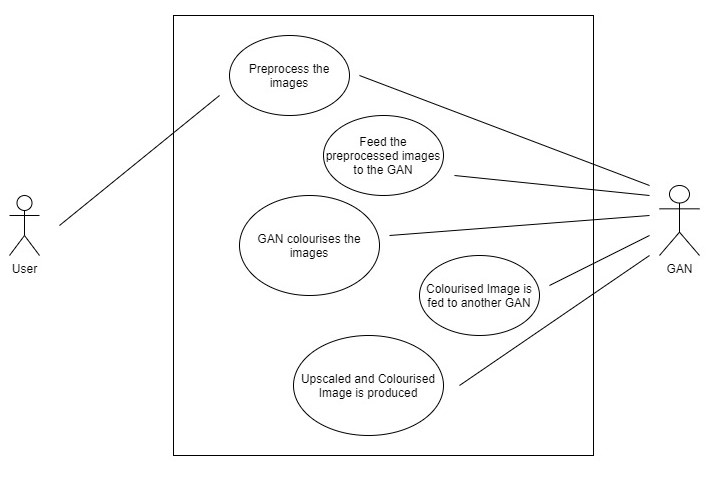
\includegraphics[width=\textwidth]{figures/use.jpg}}
	  \caption{Use case diagram}
	  \label{fig:usecase_dig}
	\end{figure}
\end{center}

\section{System Requirements}
\subsection{Hardware Resources Required}
\hspace*{0.25 in}The project is based Machine Learning, and the use of Tensorflow-GPU brought forward the need for a very high end hardware. Google Colab (or Colaboratory) is a free Jupyter notebook environment offered by Google which runs notebooks from Python kernels and uses Google Drive for storage.
\begin{table}[!htbp]
\begin{center}
\def\arraystretch{1.5}
  \begin{tabular}{| c | c | c | c |}
\hline
Sr. No. &	Parameter &	Minimum Requirement & Justification \\
\hline
1 &	GPU type &	 NVIDIA CuDA enabled GPU  & Training the model\\
\hline
2 &	GPU memory  &	$>$6 GB &  Batch training\\
 \hline
\end{tabular}
 \caption { Hardware Requirements }
 \label{tab:hreq}
\end{center}

\end{table}


%\section{Hardware Resources Required}
%The project is based Machine Learning, and the use of Tensorflow-GPU brought forward the need for a very high end hardware. Google Colab (or Colaboratory) is a free Jupyter notebook environment offered by Google which runs notebooks from Python kernels and uses Google Drive for storage.
%\begin{table}[!htbp]
%\begin{center}
%\def\arraystretch{1.5}
%  \begin{tabular}{| c | c | c | c |}
%\hline
%Sr. No. &	Parameter &	Minimum Requirement & Justification \\
%\hline
%1 &	CPU Speed &	 Intel(R) Xeon(R) CPU @ 2.20GHz  & Training the model on CPU\\
%\hline
%2 &	GPU  &	Nvidia K80-12GB-0.82GHz &  To train model on GPU\\
%3 &	RAM  &	12GB &  To load the Dataset\\
% \hline

%  \hline
%\end{tabular}
%\caption { Hardware Requirements }
% \label{tab:hreq}
%\end{center}
%\end{table}

\pagebreak

\subsection{Software Resources Required}
Platform :
\begin{enumerate}
\item Operating System: Windows/Linus
\item IDE: Jupyter Notebook
\item Programming Language: python3, javascript
\item Frameworks: Node.js, Tensorflow, plotting libraries, openCV
\end{enumerate}

\subsection{Functional Requirements:}
\begin{itemize}
	\item Data Scraping and Processing: The data pipeline should output a usable image which is RGB and has a minimum dimension of $256 \times 256$
	\item Colorization: The system should output a colorized version of the given grayscale input image
	\item Super-Resolution: The system should output a 4 times upscaled image of the input
\end{itemize}

\subsection{Non Functional Requirements:}
\begin{itemize}
  \item Accessibility: The dataset generated would be accessible for everyone to access in open source.
	\item	Availability: The code would be available on github
  \item Performance: The performance of all the GANs is recorded.
\end{itemize}

\clearpage


\chapter{Project Plan}

\section{Project Estimates}
                 Use Waterfall model and associated streams derived from assignments 1,2, 3, 4 and 5( Annex A and B) for estimation.
\subsection{Reconciled Estimates}
\subsubsection{Cost Estimate}
\hspace*{0.25 in}
The model followed is the Constructive Cost Model (COCOMO) for estimating the
efforts required in the completion of the porject. Like all estimation models, the
COCOMO model requires sizing information. This information can be specified in
the form of:
\begin{itemize}
  \item Object Point
  \item Function Point(FP)
  \item Lines of Source Code(KLOC)
\end{itemize}
For our project, sizing information in the form of Lines of Source Code is used. The
total lines of code,\\
KLOC = 1000\\
Equations: The initial effort(Ei) in man-months is calculated using equations:\\

\[E=ax(KLOC)^b\]
\hspace*{0.25 in}where, a = 3.0, b = 1.12, for a semi-detached project
E = Efforts in person-hours\\
E = 4.5 PM\\
\[D=ax(E)^b\]
Where, a = 2.5,\\
b = 0.35, for a semi-detached project\\
D = Duration of Project in months\\
D = 12 Months\\

\subsubsection{Time Estimates}
\[C=D*Cp*hrs\]
Where, C = Cost of project\\
D = Duration in Hours\\
Cp = Cost incurred per person-hour\\
hrs = hours\\
Total of 4.5 person-months are required to complete the project successfully.\\
Duration of Project D = 12 Months\\
The approximate duration of the project is 12 months\\

\subsection{Project Resources}
          Project resources  [People, Hardware, Software, Tools and other resources] based on Memory Sharing, IPC, and Concurrency derived using appendices to be referred.

\section{Risk Management }
This section discusses Project risks and the approach to managing them.
\subsection{Risk Identification}
\begin{enumerate}
  \item Dataset needs to be processed in order to get clean data
  \item Vanishing Gradients
  \item Mode Collapse
  \item Failure to Converge
\end{enumerate}

\subsection{Risk Analysis}
The risks for the Project can be analyzed within the constraints of time and quality

\begin{table}[!htbp]
\begin{center}
%\def\arraystretch{1.5}
\def\arraystretch{1.5}
\begin{tabularx}{\textwidth}{| c | X | c | c | c | c |}
\hline
\multirow{2}{*}{ID} & \multirow{2}{*}{Risk Description}	& \multirow{2}{*}{Probability} & \multicolumn{3}{|c|}{Impact} \\ \cline{4-6}
	& & &	Schedule	& Quality	& Overall \\ \hline
1	& Garbage images in dataset	& Medium	& Low	& High	& High \\ \hline
2	& Vanishing Gradients 	& Low	& Low	& High	& High \\ \hline
\end{tabularx}
\end{center}
\caption{Risk Table}
\label{tab:risk}
\end{table}


\begin{table}[!htbp]
\begin{center}
%\def\arraystretch{1.5}
\def\arraystretch{1.5}
\begin{tabular}{| c | c | c |}
\hline
Probability & Value &	Description \\ \hline
High &	Probability of occurrence is &  $ > 75 \% $ \\ \hline
Medium &	Probability of occurrence is  & $26-75 \% $ \\ \hline
Low	& Probability of occurrence is & $ < 25 \% $ \\ \hline
\end{tabular}
\end{center}
\caption{Risk Probability definitions \citep{bookPressman}}
\label{tab:riskdef}
\end{table}

\begin{table}[!htbp]
\begin{center}
%\def\arraystretch{1.5}
\def\arraystretch{1.5}
\begin{tabularx}{\textwidth}{| c | c | X |}
\hline
Impact & Value	& Description \\ \hline
Very high &	$> 10 \%$ & Schedule impact or Unacceptable quality \\ \hline
High &	$5-10 \%$ & Schedule impact or Some parts of the project have low quality \\ \hline
Medium	& $ < 5 \% $ & Schedule impact or Barely noticeable degradation in quality Low	Impact on schedule or Quality can be incorporated \\ \hline
\end{tabularx}
\end{center}
\caption{Risk Impact definitions \citep{bookPressman}}
\label{tab:riskImpactDef}
\end{table}

\subsection{Overview of Risk Mitigation, Monitoring, Management}
Following are the details for each risk
\begin{table}[!htbp]
\begin{center}
%\def\arraystretch{1.5}
\def\arraystretch{1.5}
\begin{tabularx}{\textwidth}{| l | X |}
\hline
Risk ID	& 1 \\ \hline
Risk Description	& There are Garbage images in dataset which can lead to improper training of discriminator. It can lead to undesired outputs \\ \hline
Category	& Pre processing. \\ \hline
Source	& Software requirement Specification document. \\ \hline
Probability	& Low \\ \hline
Impact	& High \\ \hline
Response	& Mitigate \\ \hline
Strategy	& To manually remove garbage images from the dataset  \\ \hline
Risk Status	& Occurred \\ \hline
\end{tabularx}
\end{center}
%\caption{Risk Impact definitions \cite{bookPressman}}
\label{tab:risk1}
\end{table}

\begin{table}[!htbp]
\begin{center}
%\def\arraystretch{1.5}
\def\arraystretch{1.5}
\begin{tabularx}{\textwidth}{| l | X |}
\hline
Risk ID	& 2 \\ \hline
Risk Description	& If discriminator is too good , then generator training can fail due to Vanishing gradients  \\ \hline
Category	& Requirements \\ \hline
Source	& Software Design Specification documentation review. \\ \hline
Probability	& Low \\ \hline
Impact	& High \\ \hline
Response	& Mitigate \\ \hline
Strategy	& Wasserstein loos and Modifed minimax loss are desigend to prevent vanishing gradients.  \\ \hline
Risk Status	& Identified \\ \hline
\end{tabularx}
\end{center}
\label{tab:risk2}
\end{table}

\newpage
\section{Project Schedule}
\subsection{Project task set}
Major Tasks in the Project stages are:
\begin{itemize}
  \item Task 1: Collecting Dataset
  \item Task 2: Cleaning Dataset
  \item Task 3: Creating GAN model of image colorization and super-resolution
  \item Task 4: Training  the GAN model
  \item Task 5: Fine tuning the GAN model
\end{itemize}


\section{Team Organization}
\begin{itemize}
\item Team of 4 members
\item 1 Project guide
\item 1 Project coordinator
\end{itemize}
\subsection{Team structure}
Team of 4 members

\subsection{Management reporting and communication}
\begin{itemize}
\item Weekly meeting with guide about the work
\item Weekly meeting among team for updates and work distribution
\item Daily updates on work progress
\end{itemize}


\chapter{System Design}
 \section{Introduction}
\hspace*{0.25 in}The project is largely inspired by Christian Ledig's SRGAN paper \citep{ledig2017photorealistic} and \citet{dong2014super}'s implementation of SRGANs using Tensorflow. \citet{dahl2016automatic}'s introduction of residual encoding using VGG architecture and adaptation of GANs as conditional GANs by \citet{mirza2014conditional} proved to be quite effective for implementing colorization of images. We provide detailed architectural design for each respective GANs and other networks that it will be compared with.
\section{Architectural Design}
\hspace*{0.25 in}Generative Adversarial Networks (GANs) have two competing neural network models. The generator takes in the input and generates fake images. The discriminator gets the image from both the generator and the label along with the grayscale image and it determines which pair contains the real colored image. During training, the generator and the discriminator are playing a continuous game. At each iteration, generator produces a more realistic photo, while the discriminator gets better at distinguishing the fake photos. Trained in a minimax fashion, the goal is to train a generator that produces data that is indistinguishable from the real data.
	\subsection{Image Colorization}
	\hspace{0.4 in}Both the generator and discriminator are conditioned on the input $x$ with conditional GAN. Let the generator be parameterized by $\theta_g$ and the discriminator be parameterized by $\theta_d$. The minimax objective function can be defined as:
	\[
		\min_{\theta_g}\max_{\theta_d}\Big[\mathbb{E}_{x,y\sim p_{data}} \log D_{\theta_d}(x,y) + E_{x\sim p_{data}} \log(1 - D_{\theta_d}(x, G_{\theta_g}(x))\Big]
	\]

	Where, $G_{\theta_{g}}$ is the output of the generator and $D_{\theta_d}$ is the output of the discriminator.
	We're currently not introducing any noise in our generator to keep things simple for the time being. Also, we consider $L1$ difference between input $x$ and output $y$ in generator. On each iteration, the discriminator would maximize $\theta_d$ according to the above expression and generator would minimize $\theta_g$ in the following way:
	\[
		\min_{\theta_g}\Big[-\log(D_{\theta_d}(x,G_{\theta_g}(x)))+\lambda \Vert G_{\theta_g}(x) - y \Vert_1 \Big]
	\]

	With GAN, if the discriminator considers the pair of images generated by the generator to be a fake photo (not well colored), the loss will be back-propagated through discriminator and through generator. Therefore, generator can learn how to color the image correctly. At the final iteration, the parameters $\theta_g$ will be used in our generator to color grayscale images.

  \begin{center}
	\begin{figure}[!htbp]
		\centering
		\fbox{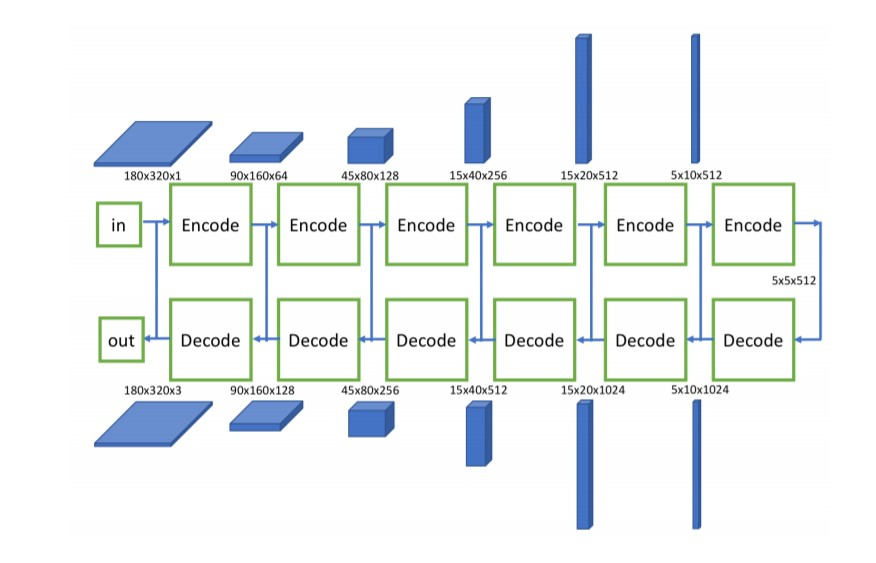
\includegraphics[width=\textwidth]{figures/encoder_decoder_generator_color.jpg}}
	  \caption{Encoder-Decoder ConvNets in Generator}
	  \label{fig:gen_color-dig}
	\end{figure}
\end{center}

  \begin{center}
	\begin{figure}[!htbp]
		\centering
		\fbox{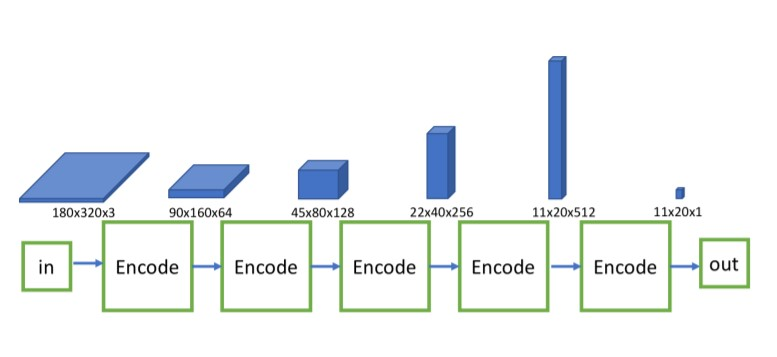
\includegraphics[width=\textwidth]{figures/discriminator_color.jpg}}
	  \caption{Discriminator}
	  \label{fig:disc_color-dig}
	\end{figure}
  \end{center}

\pagebreak

  \subsection{Image Super-resolution}
\hspace{0.4 in}We use the SRResNet as the generator in the SRGAN model as used by \citet{ledig2017photorealistic}. It contains both the residual blocks and the skip connections, as seen in Figure \ref{fig:srgan-dig}. Within each residual block, there are two convolution layers followed by a Batch Normalization layer and a parametric ReLU layer. Finally, the image is then upscaled 4 times using two sub-pixel convolution layers \citep{shi2016subpixel}.
	\begin{center}
	\begin{figure}[!htbp]
		\centering
		\fbox{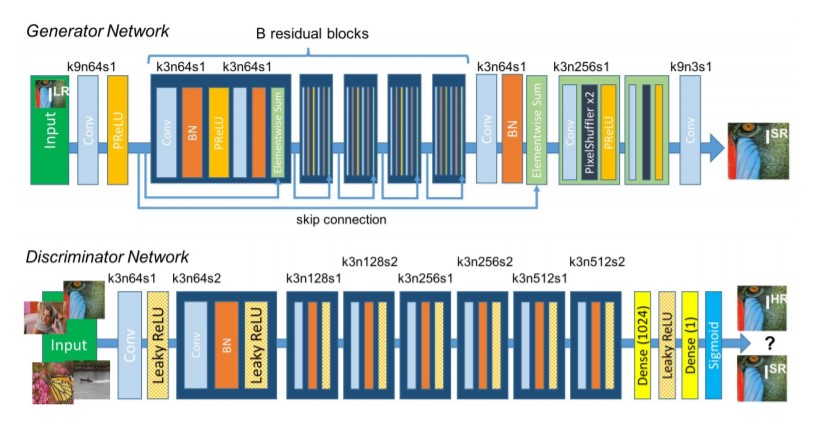
\includegraphics[width=\textwidth]{figures/ledig_srgan_architecture.jpg}}
	  \caption{SRGAN model: SRResNet generator and discriminator}
	  \label{fig:srgan-dig}
	\end{figure}
  \end{center}
\hspace*{0.25 in}The goal of the generator is to produce high resolution images that will fool the discriminator of the GAN into thinking that it is receiving real instead of fake images. On the other hand the discriminator's goal is to classify the images it has received as either real images or generated images from the generator. The GANs objective function is a minimax game as mentioned in the previous section. We define the minimax function for this task with trivial changes in notation and express it as:

\[
		\min_{\theta_g}\max_{\theta_d}\mathbb{E}_{I^{HR}\sim p_{train}(I^{HR})}\big[ \log D_{\theta_d}(I^{HR})\big] + \mathbb{E}_{I^{LR}\sim p_{g}(I^{LR})}\big[\log(1 - D_{\theta_d}(G_{\theta_g}(I^{LR})))\big]
	\]
	where, $I^{HR}p_{train}(I^{HR})$ are the high resolution images. $I^{LR}p_g(I^{LR})$ are the input low resolution images, $G_{\theta_g}$ is the output of the generator and $D_{\theta_d}$ is the output of the discriminator. We use the perpetual loss function for VGG based content losses introduced by \citet{ledig2017photorealistic} which is a weighted sum of a content loss $l^{SR}_X$ and an adversarial loss component $(10^{-3}l^{SR}_{Gen})$.

	For the content loss, we aim to use the VGG loss introduced by \citet{ledig2017photorealistic} which is the euclidean distance between the feature representations of a reconstructed image $G_{\theta_g}(I^{LR})$ and the reference image $I^{HR}$:
	$$
		l^{SR}_{VGG_{i,j}} = \frac{1}{W_{i,j}H_{i,j}} \sum_{x=1}^{W_{i,j}}\sum_{y=1}^{H_{i,j}}\big(\phi_{i,j}(I^{HR})_{x,y}-\phi_{i,j}(G_{\theta_g}(I^{LR}))_{x,y}\big)^2
	$$
	where $W_{i,j}$ and $H_{i,j}$ represent the dimensions of the respective feature maps within VGG19 network. The adversarial generative loss $l^{SR}_{Gen}$ is defined on the probabilities of the discriminator $D_{\theta_d}(G_{\theta_g}(I^{LR}))$ over all the training samples as:
	$$
		l^{SR}_{Gen} = \sum_{n=1}^{N} - \log D_{\theta_d}(G_{\theta_g}(I^{LR}))
	$$

	$D_{\theta_d}(G_{\theta_g}(I^{LR}))$ is the probability that the reconstructed image $G_{\theta_g}(I^{LR}))$ is a natural HR image. For beter gradient behavior, we minimize $-\log D_{\theta_d}(G_{\theta_g}(I^{LR}))$ instead of $\log \big[1-D_{\theta_d}(G_{\theta_g}(I^{LR}))\big]$.
	
\pagebreak
	
\section{Mathematical Model}

\subsection{Artificial Neural Networks}
\hspace{0.25 in}Figure \ref{fig: ANN} shows a schematic of the simplest multi-layer perceptron network, i.e. a feed-forward neural network. The network is composed of an input layer, hidden layers and output layer. Define $a_i^\ell$ as the $i^{th}$ neuron of the $\ell^{th}$ layer and $a_j^{\ell+1}$ as the $j^{th}$ neuron of the $(\ell+1)^{th}$ layer and $w_{ij}^\ell, b_j^\ell$ is the weight and bias connecting the two neurons, then the output of the $\ell^{th}$ layer is given by:
\begin{equation}
    a^{\ell+1}_j = g(\sum_{i \in N^\ell}(w_{ij}^{\ell}a_i^{\ell} + b_j^{\ell}))
    \label{ANN_activation}
\end{equation}

\begin{figure}[!htb]
    \centering
    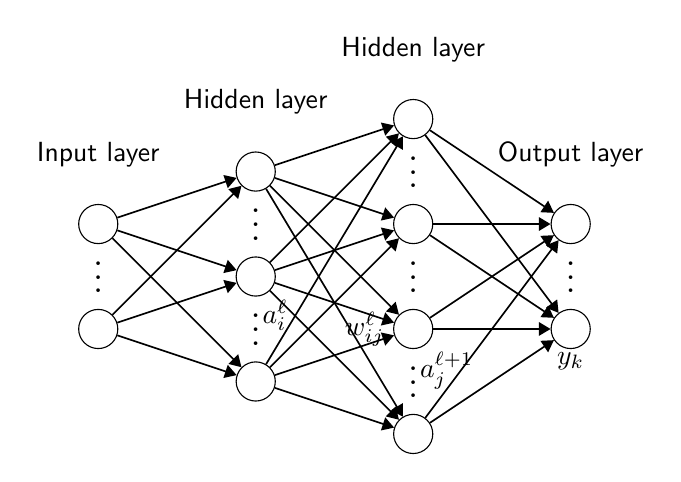
\begin{tikzpicture}[neuron/.style={circle,inner sep=.5em,draw},
    neuron missing/.style={
    scale=1.25,
    text height=0.333cm,
    execute at begin node=$\vdots$,
  }]
 \begin{scope}[x=2cm,y=1.333cm]  
 \foreach \X/\Y [count=\Z,remember=\Y as \LastY] in {Input/2,Hidden/3,Hidden/4,Output/2} 
 {\foreach \YY in {1,...,\Y}
 {\node[neuron] (n-\Z-\YY) at (\Z,-\YY+\Y/2+1/2) {};
 \ifnum\YY=1
  \node[above=1em of n-\Z-\YY,font=\sffamily] {\X\ layer};
 \else
  \path (n-\Z-\the\numexpr\YY-1) -- (n-\Z-\YY) 
   node[midway,neuron missing] {};
 \fi
 \ifnum\Z>1
  \foreach \YYY in {1,...,\LastY}
  {\draw[-{Triangle},semithick] (n-\the\numexpr\Z-1\relax-\YYY) -- (n-\Z-\YY) ;}
 \fi
 }}
 \end{scope} 
 \path[nodes={inner sep=1pt}]
    (n-2-2.-80) node[below right]{$a_i^\ell$} 
    (n-3-3.-80) node[below right]{$a_j^{\ell+1}$}
    (n-3-3.west) node[left=2pt]{$w_{ij}^{\ell}$}
    (n-4-2.-90) node[below]{${y_k}$};
\end{tikzpicture}
    \caption{A feed forward neural network}
    \label{fig: ANN}
\end{figure}

The loss is calculated using a loss function such as cross entropy function especially for binary classification.
\begin{equation}
    loss(y',y) = -y\log{y'} - (1-y)\log{(1-y')}.
    \label{ANN_loss}
\end{equation}
where $y' \in \{0,1\}, y \in (0,1)$. This objective is to minimize this cross entropy over a batch of all training data. This is done using gradient descent where the parameters viz. weights and biases are updated to reduce the overall cross entropy loss.

\subsection{Convolutional Neural Networks}
\hspace*{0.25 in}A convolution is a linear operation that can be viewed as a multiplication or dot product of matrices. The input is a tensor of shape $height$ x $width$ x $channels$ and the convolution operation abstracts the image to a feature map (also called a kernel) of shape $kernel size$ x $kernel size$ x $kernel channels$. The layers can be computed by:
\begin{equation}
    a^{\ell+1}_j = g(\sum_{i \in F_j}(a_i^\ell \times k_{ij}^{\ell+1} + b_j^{\ell+1}))
    \label{Convolution}
\end{equation}
where $\ell$ is the layer, g is the activation function ReLU, $F_j$ is the receptive field, k is the convolutional kernel and b is the bias.

\subsection{Residual Networks}
\begin{figure}
    \centering
    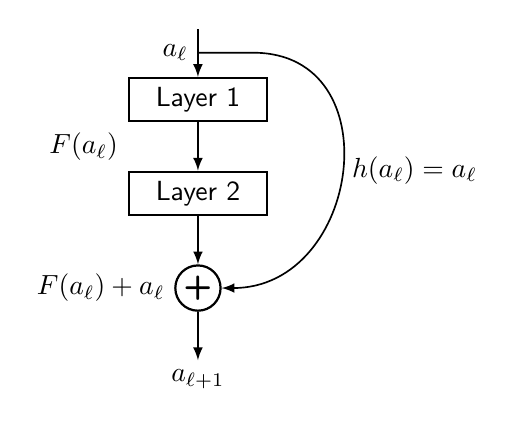
\begin{tikzpicture}[box/.style={draw,thick,minimum width=5em,minimum
    height=1.2em},arj/.style={semithick,-latex}]
  \begin{scope}[start chain=A going below,oc/.style={join=by arj,on chain},
    font=\sffamily,node distance=1.75em]
   \node[box,oc]{Layer 1};
   \node[box,oc,label={north west:{$F(a_\ell)$}}]{Layer 2};
   \node[circle,oc,draw,thick,node font=\bfseries\large,inner sep=1pt,
    label={left:{$F(a_\ell)+a_\ell$}}]{+};
   \node[oc]{$a_{\ell+1}$};
  \end{scope}   
  \draw[arj,latex-] (A-1.north) -- ++ (0,1.75em)
      coordinate[midway,label=left:{$a_\ell$}](aux);
  \draw[arj] (aux) -- ++ (2em,0) to[out=0,in=0,looseness=1.5]
  node[midway,right]{$h(a_\ell)=a_\ell$}(A-3);    
\end{tikzpicture}
    \caption{Residual Block}
    \label{fig: residual block}
\end{figure}
\hspace*{0.25 in}Figure \ref{fig: residual block} shows a building block of a residual network. The residual blocks can be expressed mathematically as follows. Let $h(a)$ be an underlying mapping that is to be fit by a set of layers, where $a$ is the input to these layers. If we hypothesize that multiple non-linear transformations by these layers can approximate the layer functions, then one can also hypothesize that a similar approximation can be made for the residual functions, i.e. $h(a) - a$, which have the same input and output dimensions. So instead of letting the underlying mapping be $h(a)$ we approximate a residual function $F(a) = h(a) - a$. Thus, the actual function becomes $h(a) = F(a) + a$. We can achieve this approximation in a feed forward neural network using a series of skip connections that perform identity mapping and jump over a few layers. Adding the outputs of these two connections gives the final output layer. Thus, the residual unit can be defined as,
\begin{equation}
    a_{\ell+1} = h(a_\ell) + F(a_\ell, W_\ell)
    \label{Residual unit}
\end{equation}
where $a_{\ell+1}$ and $a_\ell$ represent the input and output for the $\ell^{th}$ layer and $F$ is the residual function. The $h$ denotes the operation in the identity mapping. The output of the layer is generally processed using an activation function such as ReLU. Let $f$ be the ReLU activation and replacing $F$ with the definition of feed forward activation, the residual block thus can be defined as,
\begin{equation}
    a_{\ell+1} = f(h(a_\ell) + W_2f(W_1a_\ell))
    \label{Residual unit redefined}
\end{equation}
\hspace*{0.25 in}For the sake of simplicity, we consider no operation being performed in the identity mapping. Thus, equation \ref{Residual unit} and equation \ref{Residual unit redefined} become,
\begin{equation}
    a_{\ell+1} = f(a_\ell + F(a_\ell, W_\ell))
    \label{Final Residual notation}
\end{equation}

\subsection{Generative Adversarial Networks}
\hspace*{0.25 in}A generative network, $G$, is supposed to learn the underlying distribution of a latent space, Y. Instead of visually assessing the quality of network outputs and judge how we can adapt the network to produce convincing results, we incorporate automatic tweaking during training by introducing a discriminative network $D$. The network D takes in both the fabricated outputs generated by G and real inputs from the underlying distribution Y. The network produces a probability of the image belonging to the real or fabricated space.

  Let $x \in X$ be a low resolution/grayscale image and $y \in Y$ be it's underlying distribution from the latent space Y. Generator $G$ takes in input $x$ and produces an output $\hat{y}$. We define the mapping $x \rightarrow \hat{y}$ in the following manner:
  $$G(x) = \hat{y}$$

 The discriminative network D is fed the fabricated mapping $x \rightarrow \hat{y}$ and the underlying distribution of $x$ i.e. $y \in Y$. The network D then produces a result that is a probability distribution of the input space indicating the class of the image that it thinks the input belongs to. We define this as:
 $$D\big(G(x),y\big) = p$$
 where $p \in (0,1)$ is the probability that the image is fabricated or real.
With conditional GAN, both generator and discriminator are conditioning on the input $x$. Let the generator be parameterized by $\theta_g$ and the discriminator be parameterized by $\theta_d$. The minimax objective function can be defined as:
	\[
		\min_{\theta_g}\max_{\theta_d}\Big[\mathbb{E}_{x,y\sim p_{data}} \log D_{\theta_d}(x,y) + E_{x\sim p_{data}} \log(1 - D_{\theta_d}(x, G_{\theta_g}(x))\Big]
	\]

	Where, $G_{\theta_{g}}$ is the output of the generator and $D_{\theta_d}$ is the output of the discriminator.
	We're currently not introducing any noise in our generator to keep things simple for the time being. Also, we consider $L1$ difference between input $x$ and output $y$ in generator. On each iteration, the discriminator would maximize $\theta_d$ according to the above expression and generator would minimize $\theta_g$ in the following way:
	\[
		\min_{\theta_g}\Big[-\log(D_{\theta_d}(x,G_{\theta_g}(x)))+\lambda \Vert G_{\theta_g}(x) - y \Vert_1 \Big]
	\]
	

\pagebreak
\section{UML Diagrams}

\subsection{Activity Diagram:}

    \begin{figure}
    \begin{center}
    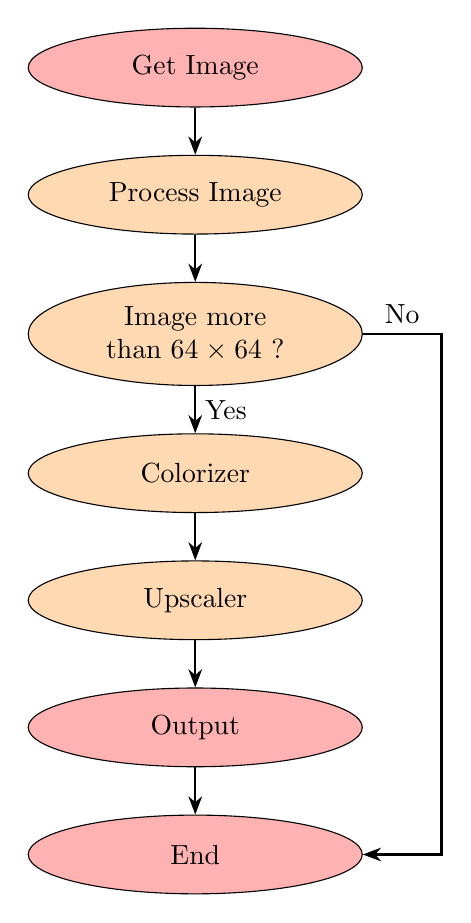
\begin{tikzpicture}[FlowChart,
  node distance = 6mm and 12mm,
    start chain = going below]

% nodes
\node (begin)   [coordinate] {dot};
\node (start)   [startstop] {Get Image};
\node (proc01)  [process]   {Process Image};
\node (dec01)   [process]  {Image more than $64 \times 64$ ?};
\node (proc03)  [process]   {Colorizer};
\node (proc04)  [process]   {Upscaler};
\node (end)     [startstop] {Output};
\node (end2)     [startstop] {End};
% extra paths
\path           (dec01) -- node[right] {Yes} (proc03);
\draw [arrow]   (dec01.east) -- node[above] {No} ++(1cm,0) |- (end2);

    \end{tikzpicture}
    \caption{Activity Diagram}
    \label{fig:Activity Diagram}

        \end{center}
    \end{figure}


\clearpage
\subsection{State Transition Diagram:}


    \begin{figure}
    \begin{center}
    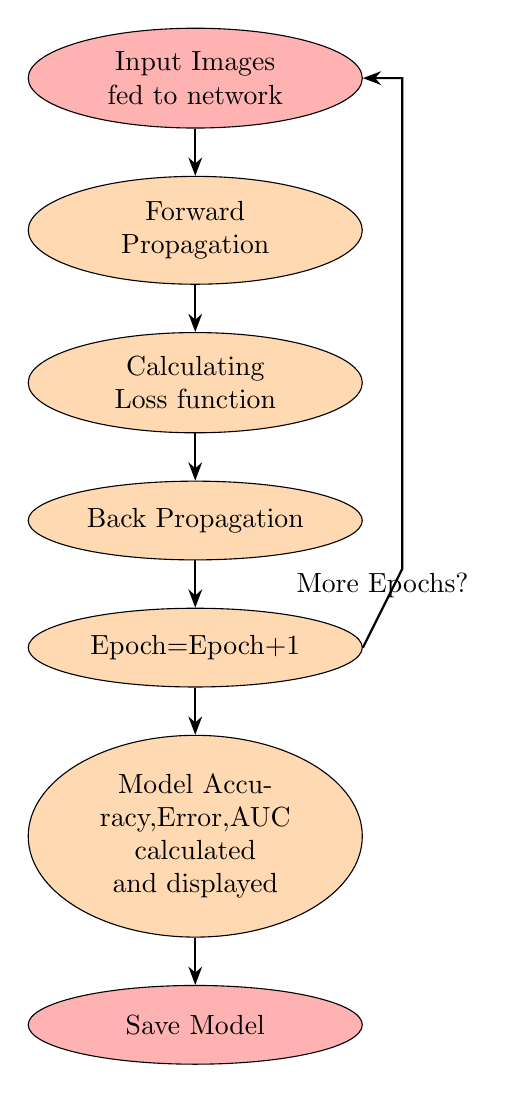
\begin{tikzpicture}[FlowChart,
  node distance = 6mm and 12mm,
    start chain = going below]

% nodes
\node (begin)   [coordinate] {dot};
\node (start)   [startstop] {Input Images fed to network};
\node (proc01)  [process]   {Forward Propagation};
\node (dec01)   [process]  {Calculating Loss function};
\node (proc03)  [process]   {Back Propagation};
\node (proc04)  [process]   {Epoch=Epoch+1};
\node (proc05)  [process]   {Model Accuracy,Error,AUC calculated and displayed};
\node (end2)  [startstop]   {Save Model};
% extra paths

\draw [arrow]   (proc04.east) -- node[above] {More Epochs?} ++(0.5cm,1) |- (start);

    \end{tikzpicture}
    \caption{State Transition Diagram}
    \label{fig:State Transition Diagram}
    \end{center}
    \end{figure}



\chapter{Project Implementation}
\section{Overview of Project modules}
\hspace{0.25 in}To gather data, the primary module implemented was a data scraper written in node.js which uses puppeteer(headless chrome) to scrape the entire HLA(Hubble Legacy Archive) with the described RA and Dec co-ordinates of the night sky. The module ensured that, out of the entire data available in the Legacy Archive, a certain format of images would be downloaded and stored appropriately. After gathering the data, it was apparent that there were many other processed images present on the Hubble main and other citizen science projects conducted with Hubble Space Telescope. To scrape these, a python script using selenium was written so as to efficiently scrape processed images which had a minimum dimensions of $256 \times 256 \times 3$. With the data gathered, the main components, i.e. the models were built.\\
\hspace*{0.25 in}The project entails a standard set of GAN modules, broadly, a data pre-processing pipeline, a training pipeline, intermediate state logging and a testing pipeline.
\begin{itemize}
	\item \textbf{Data Pre-processing}
	\begin{itemize}
		\item The data pre-processing pipeline is an important part of the data pipeline that feeds the data to the training pipeline
		\item The images, being too large to be loaded into the memory simultaneously, had to be loaded through a data generator
		\item We implement an instance of \texttt{Keras Image Data Generator} to convert the raw data into training data
		\item We create two \textit{data generators}, one for generating gray scale images and the other for generating subsequent RGB image
		\item We create another data pre-processor that converts the given RGB image into L*a*b color space
		\item The images are then resized to a dimension of $64 \times 64$ 
		\item We get a vector of image batches which will be the input to the training pipeline
	\end{itemize}
	
	\item \textbf{Training Pipeline}
	\begin{itemize}
		\item The training pipeline consists of multiple phases
		\item Initially, we build the basic neural networks for generator and discriminator networks, i.e. a tensor graph which will function as a computation graph for forward and backward propagation
		\item The next step is selection of an optimizing algorithm
		\item After selection of optimizer, a training pipeline is implemented which includes running a session of forward and backward propagation throughout the computation graph and optimizing the trainable variables of the networks
	\end{itemize}
	\item \textbf{Intermediate state logging}
	\begin{itemize}
		\item Deep Learning models use up a lot of computational resources and are time consuming to train
		\item Thus, it is essential to set up methods that will extract intermediate states of the model while it is still in the training loop
		\item These methods are often termed as 'callbacks' and we implement different callbacks to ensure availability of training history, weights and intermediate results during documentation
		\item A csv logger logs the metrics at the end of each epoch into a csv file for model evaluation
		\item The model weights are saved if the loss metric improves than the earlier epoch. We implement a mechanism for early stopping where the training loop exits if the model appears to have converged
	\end{itemize}
	\item \textbf{Testing pipeline}
	\begin{itemize}
		\item Model testing is performed on a testing dataset that is different than the original dataset
		\item Testing pipeline is implemented by using the saved weights of the trained model and the images are processed through the entire dataset
		\item We evaluate the images qualitatively as well as quantitatively using visual inspection and distance metrics
	\end{itemize}
\end{itemize}

\section{Tools and Technology used}
\hspace*{0.25 in}We use the following tools:
\begin{itemize}
	\item Data gathering: Node.js, puppeteer, selenium
	\item Data Processing: openCV, Pillow
	\item Pre-processing \& input pipeline: numpy, tensorflow-keras
	\item Model building \& training: tensorflow 2.x
	\item Model evaluation: tensorflow, numpy
	\item Visualization: matplotlib, Pillow
\end{itemize}

\section{Algorithm Details}
\subsection{Generative Networks}
\hspace*{0.25 in}A generative model is a class of statistical models that are a contrast to the classifier models dubbed as discriminative models. Informally speaking, a generative model creates new data instances based on the distribution of the data itself. Generative models tackle a more difficult task, i.e. to model data. A generative model might capture correlations among underlying distribution and draw conclusions. \cite{goodfellow2014generative} proposed the most famous type of generative model, i.e. Generative Adversarial Network, which is composed of two smaller networks called a discriminator and a generator. The generator's task is to create fake images that convince the discriminator and the discriminator usually classifies between real and fake data. 
\subsection{Adversarial Networks}
\hspace*{0.25 in}With two networks that are neural networks, the adversarial modeling framework is the most straightforward to apply. A distribution $p_g$ over data $x$ is called the generator's distribution. To learn this distribution, we define some prior noise on the input variables $p_z(z)$ and represent a mapping to a space with $G(z; \theta_g)$, where $G$ is a differential function of neural network parameterized by $\theta_g$. Another neural network $D(x;\theta_d)$ is defined such that it provides a scalar output, representing the probability that data $x$ comes from the input distribution rather than $p_g$. The goal is to train $D$ to maximize the probability of assigning the correct label to both training examples and samples from $G$. The network $G$ is trained to minimize $log(1-D(G(z))$. 

\SetAlgoNoLine%
\begin{algorithm}[!htb]
\For{number of training examples}{
\For{k steps}{
	$\bullet$ Sample minibatch of $m$ noise samples $\{z^{(1)}\dots z^{(m)}\}$ from noise prior to $p_g(z)$.\\
	$\bullet$ Sample minibatch of $m$ examples $\{x^{(1)}\dots x^{(m)}\}$ from data generating distribution $p_{data}(x)$.\\
	$\bullet$ Update the discriminator by ascending its stochastic gradient:
		$$
			\bigtriangledown_{\theta_d}\frac{1}{m}\sum_{i=1}^m\Big[ log D \Big( x^{(i)}\Big) + log \Big( 1 - D \Big( G \Big( z^{(i)} \Big) \Big) \Big) \Big]
		$$
 }
 $\bullet$ Sample minibatch of $m$ noise samples $\{z^{(1)}\dots z^{(m)}\}$ from noise prior to $p_g(z)$.\\
 $\bullet$ Update generator by descending its stochastic gradient:
 		$$
			\bigtriangledown_{\theta_g}\frac{1}{m}\sum_{i=1}^m log \Big( 1 - D \Big( G \Big( z^{(i)} \Big) \Big) \Big) 
		$$
 }
 \caption{Minibatch stochastic gradient descent training of generative adversarial networks. The number of steps to apply to the discriminator, $k$, is a hyperparameter.}
\end{algorithm}

\subsection{Conditional GANs}
\hspace*{0.25 in}As mentioned earlier, GANs are generative models that learn a mapping from a random noise vector $z$ to output $p_g$. The mapping from vector $z$ to an output image $y$ can be represented as $G: z \rightarrow y$ \citep{goodfellow2014generative}. \cite{isola2018imagetoimage} presented a new approach for GANs called Conditional GANs. Instead of learning just from a random noise vector, conditional GANs learn a mapping from input $x$ and the vector $z$ to $y$ such that $G: \{x,z\} \rightarrow y$. By doing this, we train the discriminator to do as well as possible to detect the generator's fake outputs whereas the generator is trained to produce results that are almost indistinguishable from the real data. The objective function of conditional GAN can be expressed as:
$$
		\min_{G}\max_{D}\Big[\mathbb{E}_{x,y}\big[ \log D(x,y)\big] + E_{x,z}\big[ \log(1 - D(x, G(x,z))\big]\Big]
$$

\section{Methodology}
\subsection{Image Color space}
\hspace*{0.25 in}An RGB image is essentially a rank 3 tensor of height, width and color where the last axis contains the color data of our image. The data is represented in RGB color space which has 3 numbers for every pixel indicating the amount of \textit{Red, Green, and Blue} values the pixel has. Figure \ref{rgb_colorspace} shows that in the left part of the “main image” has blue color so the blue channel of the image has higher values and turns dark.\\
\begin{figure}[!htb]
\begin{center}
	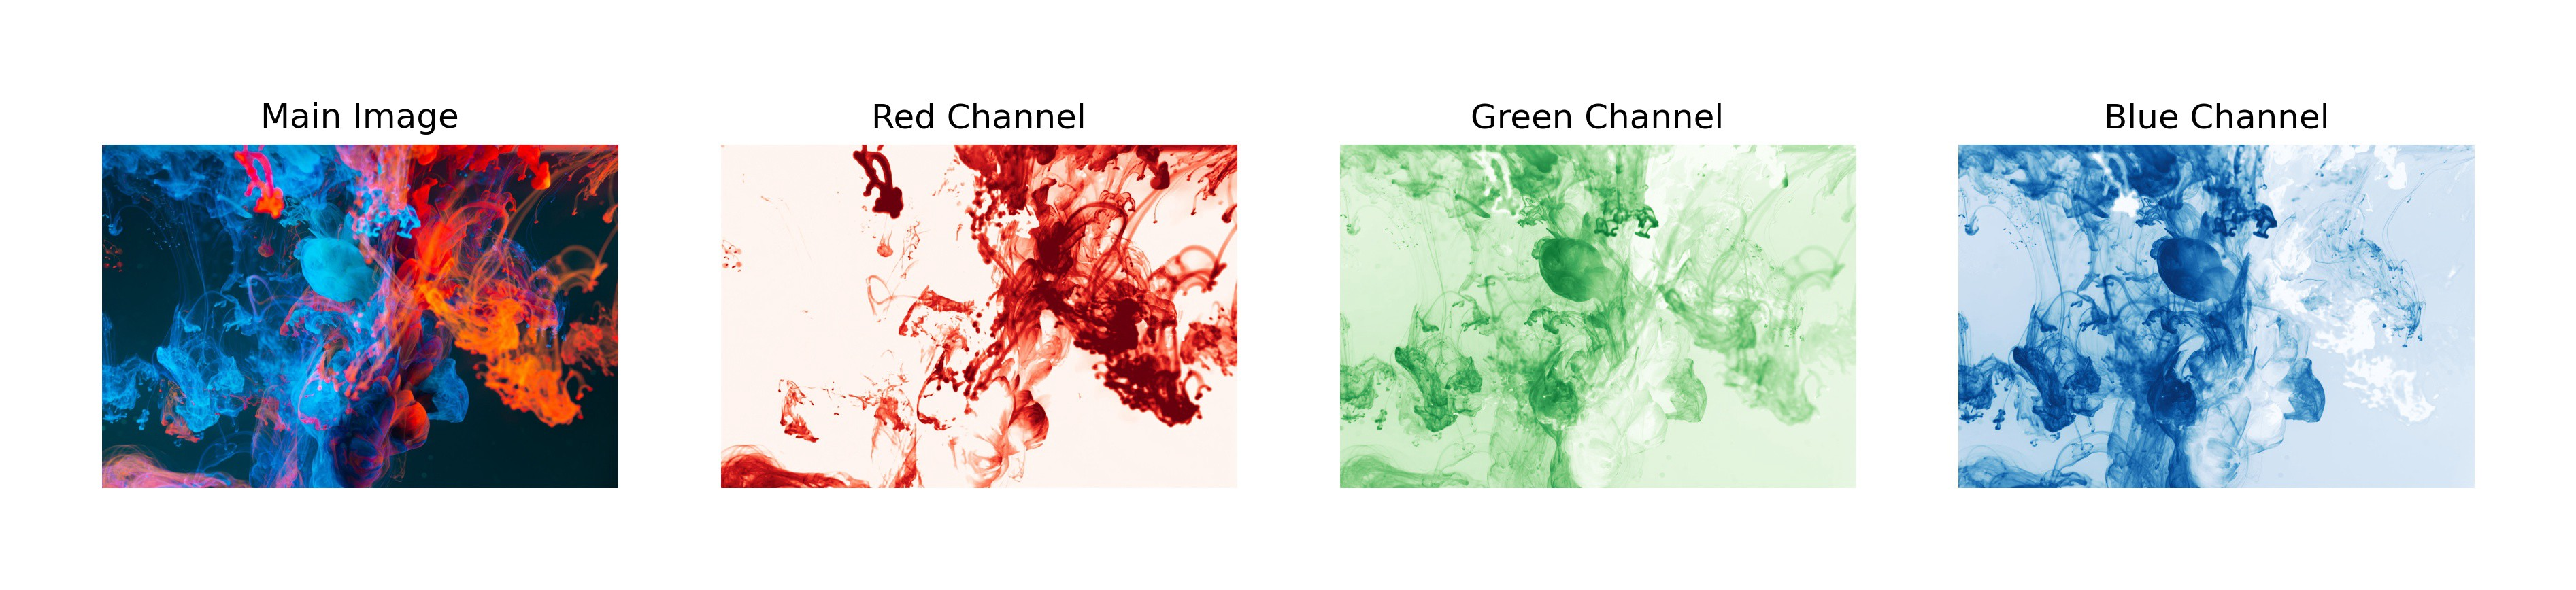
\includegraphics[width=\textwidth]{figures/rgb_colorspace}
	\caption{Reg, Green and Blue channels of an image}
	\label{rgb_colorspace}
\end{center}
\end{figure}

In \textbf{L*a*b} color space, we have three numbers for each pixel but these numbers have different meanings. The first channel, L, encodes the \textbf{Lightness} of each pixel and when we visualize this channel it appears as a black and white image. The \textbf{*a and *b} channels encode how much \textbf{green-red} and \textbf{yellow-blue} each pixel is, respectively. In the following image you can see each channel of L*a*b color space separately.

\begin{figure}[!htb]
\begin{center}
	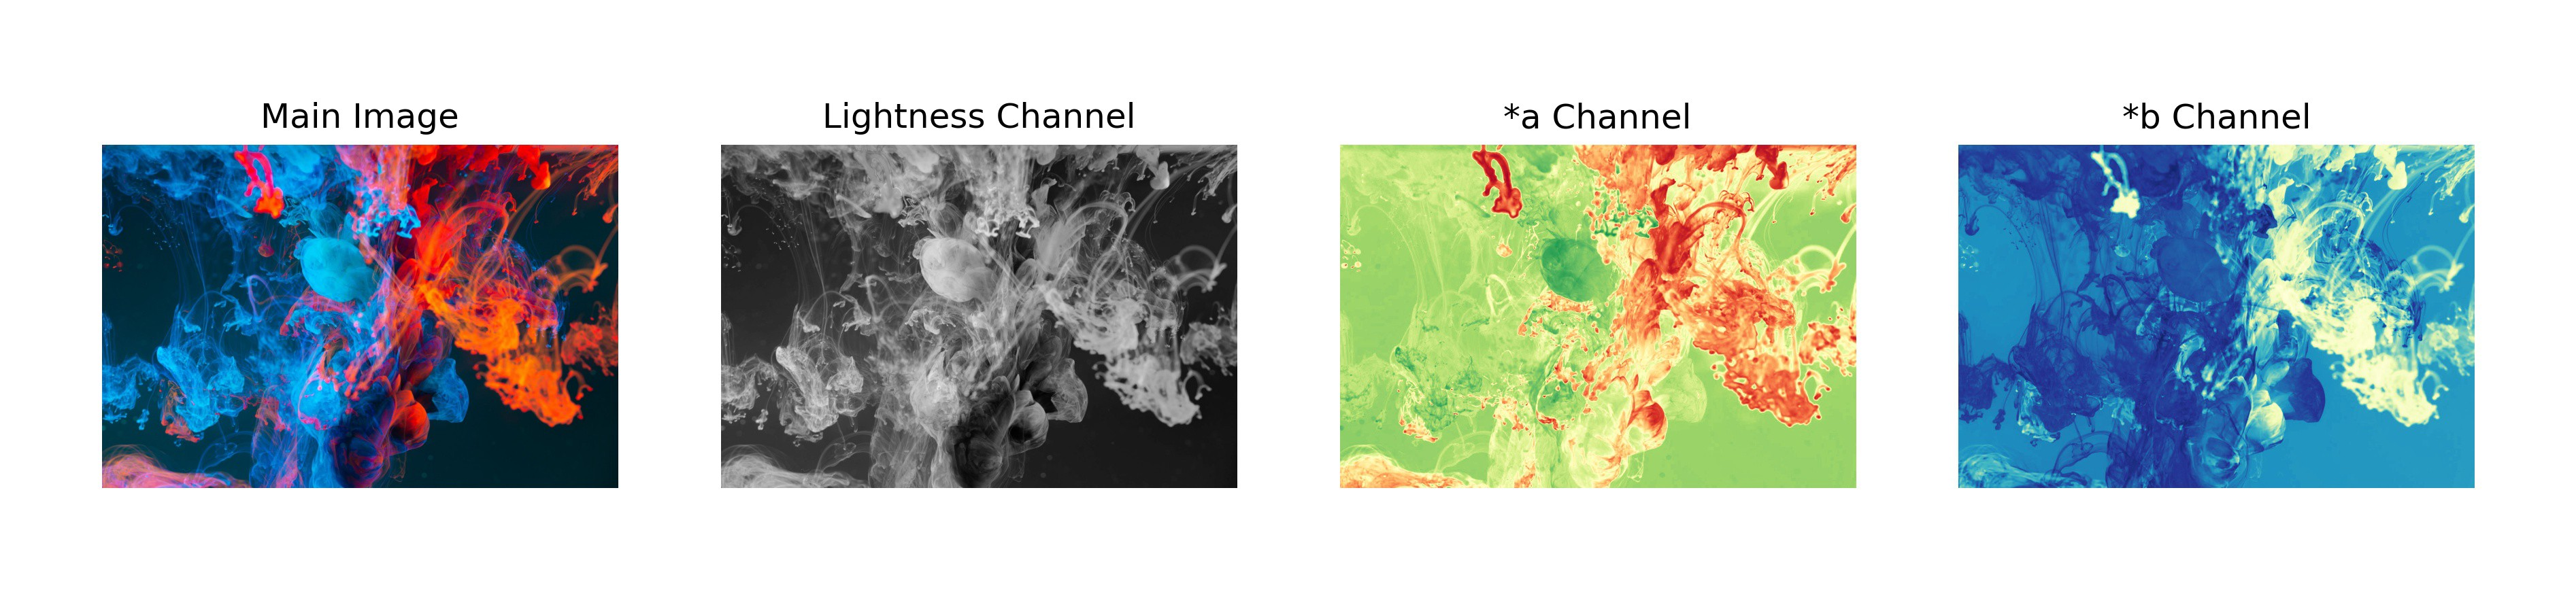
\includegraphics[width=\textwidth]{figures/Lab_colorspace}
	\caption{Lightness, *a and *b channels of the L*a*b colorspace}
	\label{lab_colorspace}
\end{center}
\end{figure}

In most of the papers listed in the Literature Survey, the L*a*b color space is widely used instead of RGB to train the models. Intuitively, to the train a model for colorization, we should give it a grayscale image and we hope that it colors it. In the L*a*b colorspace, the model is fed the L channel, which is essentially a grayscale image, and we perform computations to predict the other two channels (*a and *b). After the predictions, we concatenate the channels and get a colorful image. In case of RGB, there is a need to explicitly convert the three channels down to 1 to make it a grayscale image and then feed it to the network hoping that it predicts three numbers per pixel. This is an unstable task due to sheer increase in volume of combinations from two numbers to three.

We train models using both color spaces and empirically show the significance of the L*a*b colorspace.

\subsection{Transferred learning and model tweaking}
\hspace*{0.25 in}\cite{isola2018imagetoimage} proposed a general solution to many image-to-image translation tasks. We propose a similar methodology as proposed in the paper with a few minor tweaks, so as to significantly reduce the amount of training data needed and minimize the training time to achieve similar results. Initially, we use a U-net for the generator. The \textit{encoder} of our U-net is a pre-trained ResNet-18 network with half of it's layers clipped off so as to get feature abstractions of the middle layers. \cite{ledig2017photorealistic} showed that training the generator separately in a supervised, deterministic manner helps it generalize the mapping from the input space to outputs. The idea solves the problem of \textit{"The blind leading the blind"} that is persistent in most image-to-image translation tasks to date. \\
\hspace*{0.25 in}We decide to use the Common Objects in Context (COCO) dataset to pre-train our generator independently using the imagenet weights. This training will be supervised and the loss function used is \textit{mean absolute error} or the \textit{L1 Norm} from the target image. Even though trained deterministically,the problem of rectifying incorrect predictions still persists due to constraints over the convergence of loss metric. To combat this, we use this trained generator and train it once again in an adversarial fashion to generalize it further. We hypothesize that re-training with an adversarial will further rectify the subtle color differences that \textit{mae} couldn't solve.\\
\hspace*{0.25 in}We use a pre-trained ResNet-50 with imagenet weights as our discriminator with last few layers clipped off. The discriminative network used is something called a "Patch Discriminator" proposed by \cite{isola2018imagetoimage}. In a \textit{vanilla} discriminator proposed by \cite{goodfellow2014generative}, the network produces a scalar output, representing the probability that the data $x$ belongs to the input distribution and not the generator distribution $p_g$. \cite{isola2018imagetoimage} proposed a modification to the discriminative network so as to produce, instead of a single scalar, a vector of probabilities representing different localities of the input distribution (image) $x$. For instance, a discriminator producing a $30 \times 30$ vector represents the probabilities every receptive field that is covered by the output vector. Thus, we can localize the corrections in the image that the generator should make.\\
\hspace*{0.25 in}Finally, we use the trained generator and trained discriminator and fine-tune it to fit it on our data which is rather small in size compared to the previous datasets. We train these networks in an adversarial fashion using the conditional GAN objective function \citep{isola2018imagetoimage} and couple it with some noise introduced as the L1 norm of generated image tensor to the target image tensor. The reason behind this is to train the generator using an adversarial component while trying to minimize the Manhattan distance between the generator output and target vector space.

\chapter{Software Testing}
\section{Types of testing}
\hspace{0.25 in}We test the modules of our entire setup to ensure that the modules are performing as they're intended to. 
We perform a kind of unit testing to evaluate the output of every function in the code. 
\section{Test Cases and Test Results}
\subsection{Data Gathering and Pre-processing}
\begin{itemize}
	\item Test Case 1: Image Scraping test
	\begin{itemize}
		\item Test Case Description:\\
			The module function should scan through the legacy archive only in the described co-ordinates and scrape images that are RGB and of dimensions $256 \times 256$
		\item Status: \textbf{Pass}
	\end{itemize}
	\item Image Colorization:
	\begin{itemize}
	\item RGB Color Space:
	\begin{itemize}
		\item Test Case 2: Pre-processing System: Grayscale Images (Input distribution)
	\begin{itemize}
		\item Test Case Description:\\
			The pre-processing function takes in a stream of raw data and converts the images into a numpy array with dimensions $n \times 64 \times 64 \times 1$ where $n$ is the batch size. The output image vector should contain black \& white images
		\item Status: \textbf{Pass}
	\end{itemize}
		\item Test Case 3: Pre-processing System: Color Images (Target distribution)
	\begin{itemize}
		\item Test Case Description:\\
			The target distribution should contain color counter-parts of the respective input data. The function should output a numpy array with dimensions $n \times 64 \times 64 \times 3$ where $n$ is the batch size.
		\item Status: \textbf{Pass}

	\end{itemize}
	\end{itemize}
	\item L*a*b Color Space:
	\begin{itemize}
		\item Test Case 2: Pre-processing System: RGB to L*a*b conversion
	\begin{itemize}
		\item Test Case Description:\\
			The pre-processing function takes in a stream of raw data and converts the images into a numpy array with dimensions $n \times 64 \times 64 \times 3$ where $n$ is the batch size. The output is an image tensor in L*a*b color space. The L channel is provided for the grayscale input 
		\item Status: \textbf{Pass}
	\end{itemize}
		\item Test Case 3: Pre-processing System: L*a*b to RGB conversion
	\begin{itemize}
		\item Test Case Description:\\
			The function takes in its input as an image tensor in L*a*b colorspace. The function should output a numpy array with dimensions $n \times 64 \times 64 \times 3$ where $n$ is the batch size and the image output is converted back to the RGB space
		\item Status: \textbf{Pass}

	\end{itemize}
	\end{itemize}
	\end{itemize}
	\item Image Super-resolution:
	\begin{itemize}
		\item Test Case 4: Pre-processing System: Low Resolution Images (Input distribution)
		\begin{itemize}
			\item Test Case Description:\\
			The pre-processing function takes in the raw data and produces low resolution $64 \times 64 \times 3$ images. The output should be a numpy vector of $n$ dimensions representing the mini-batch size
			\item Status: \textbf{Pass}
		\end{itemize}
		\item Test Case 5: Pre-processing System: High Resolution Images (Target distribution)
		\begin{itemize}
			\item Test Case Description:\\
			The target distribution contains the labelled data that is a high resolution image of dimensions $256 \times 256 \times 3$. The function produces a numpy vector of size $n$ where $n$ is the size of mini-batch
			\item Status: \textbf{Pass}
		\end{itemize}
	\end{itemize}
\end{itemize}

\subsection{Model Implementation}
\begin{itemize}
	\item Image Colorization Model
	\begin{itemize}
		\item Test Case 1: Generator network
		\begin{itemize}
			\item Test Case Description:\\
			The generator network is a tensor graph implemented in tensorflow. The computation graph should have an input layer of dimensions $n \times 64 \times 64 \times 1$ which is propagated through till the final layer. The final layer output should be a tensor of dimensions $n \times 64 \times 64 \times 3$ where $n$ is the mini-batch size
			\item Status: \textbf{Pass}
		\end{itemize}
		\item Test Case 2: Discriminator network
		\begin{itemize}
			\item Test Case Description:\\
			The discriminator network is a tensor graph implemented in tensorflow. The computation graph should have an input layer of dimensions $n \times 64 \times 64 \times 3$ which is propagated through till the final layer. The final layer output should be a tensor of dimensions $n \times 30 \times 30 \times 1$ where $n$ is the mini-batch size
			\item Status: \textbf{Pass}
		\end{itemize}
	\end{itemize}
	\item Image Super-resolution Model
	\begin{itemize}
		\item Test Case 1: Generator network
		\begin{itemize}
			\item Test Case Description:\\
			The generator network is a tensor graph. The computation graph should have an input layer of dimensions $n \times 64 \times 64 \times 3$. The final layer output should be a tensor of dimensions $n \times 256 \times 256 \times 3$ where $n$ is the mini-batch size
			\item Status: \textbf{Pass}
		\end{itemize}
		\item Test Case 2: Discriminator network
		\begin{itemize}
			\item Test Case Description:\\
			The discriminator network is a tensor graph. The computation graph should have an input layer of dimensions $n \times 256 \times 256 \times 3$. The final layer output should be a tensor of dimensions $n \times 1$ where $n$ is the mini-batch size
			\item Status: \textbf{Pass}
		\end{itemize}
	\end{itemize}
\end{itemize}

\subsection{Training Loop}
\begin{itemize}
	\item Test Case 1: Forward propagation
	\begin{itemize}
		\item Test Case Description:\\
		The forward propagation function should run the computation graph over all the training samples and calculate losses of the generator and discriminator. The loss should be calculated according to the GAN objective function and final output should be the cost of the entire training epoch.
		\item Status: \textbf{Pass}
	\end{itemize}
	\item Test Case 2: Backward propagation
	\begin{itemize}
		\item Test Case Description:\\
		The backward propagation should calculate gradients of the objective function based on the cost calculated during the forward propagation. The gradients should be used to update the trainable variables of the network using gradient descent with momentum and weighted average sum, i.e. Adam.
		\item Status: \textbf{Pass}
	\end{itemize}
	\item Test Case 3: Callbacks and intermediate results logging
	\begin{itemize}
		\item Test Case Description:\\
		While training the model, the callback functionality should keep track of the intermediate training results. It should perform the following:\\
		$\bullet$ A csv file containing history of the entire training session\\
		$\bullet$ Save the model weights on a best performance basis by keeping track of the earlier losses\\
		$\bullet$ Keep track of the convergence and stop the model training if the model converges early
		
		\item Status: \textbf{Pass}
	\end{itemize}
\end{itemize}

\subsection{Evaluation system}
\begin{itemize}
	\item Model performance evaluation
	\begin{itemize}
		\item Test Case 1: Model history plotting
		\begin{itemize}
			\item Test Case Description:\\
			The function should plot the model losses throughout the training loop and present a graph of the said plot
			\item Status: \textbf{Pass}
		\end{itemize}
		\item Test Case 2: Output plotting
		\begin{itemize}
			\item Test Case Description:\\
			The function should take in the predictions by the model and save the images with their respective ground truth images for evaluation
			\item Status: \textbf{Pass}
		\end{itemize}
		\item Test Case 3: Model evaluation (L1 norm)
		\begin{itemize}
			\item Test Case Description:\\
			The function should take in two numpy vectors consisting of predicted values and ground truths respectively. The function output should be a single number consisting of the L1 norm (Manhattan distance) between the target and predictions
			\item Status: \textbf{Pass}
		\end{itemize}
	\end{itemize}
\end{itemize}


\chapter{Results}
\section{Dataset and Experimental setup}
\hspace*{0.25 in}Initially, we started by scraping the data off Hubble Legacy Archive. Using puppeteer(headless chrome), we scraped off hundreds of thousands of colorized images it has available. The Hubble Legacy archive is slow and produces grainy images with lots of noise and unprocessed images. A filter for M101 (Messier 101) galaxy rendered more than 80 thousand images with a 1 degree difference between consecutive right ascension. The data is large and has no particularly efficient way to clean without human investment. Cleaning tens of thousands of images by handpicking noiseless and well colored images is time consuming. For training the SRGAN, we need high resolution, well colored images. \\
\hspace*{0.25 in}Consequently, we scraped the Hubble Heritage project instead. The Hubble Heritage project releases the highest-quality astronomical images. They are all stitched together, colorized and processed to eliminate noise. Hubble Heritage then selects the best, most striking of these for public release. However, there are only $\sim150$ of these images that are actually useful. We scraped images from the main Hubble website as well so as to increase the amount of data we had. This provided an extra approximately $\sim1000$ images.
Each image is a JPG image with dimensions of $256\times 256$ pixels and contains 3 channels of RGB.\\
\hspace*{0.25 in}We use a mini-batch gradient descent with a batch size of 10, 16 and 32 for different iterations. We use Adam optimizer with $\beta_1 = 0.5$ and $\beta_2 = 0.999$. The generator and discriminator has a learning rate of $2e-4$ which remains constant throughout the training. We train the model with different epochs ranging between 20,50 and 100, saving the best model weights determined by L1 norm between the output of the generator and the target image. We use early stopping with a patience value of 10. The image size is $64\times64$. Our implementation is using Python, numpy, Tensorflow and tf-keras. It takes about 24 hours to complete training over the COCO dataset and about 12 to 13 hours to fit the model on given astronomical data on a NVIDIA Tesla K80 GPU.
\pagebreak
\section{Results and Discussions}
\hspace*{0.25 in}In the following section, we briefly compare and summarize the results of the implemented architectures and evaluate their performance. The evaluation is done qualitatively as well as quantitatively. We compare the performance of each model using L1 and L2 norm distance between the predictions and targets. Though unreliable, this method provides us with a somewhat decent ground to perform a comparative study and evaluate the reliability of such metrics on GAN evaluation compared to qualitative, visual evaluation.\\
\hspace*{0.25 in}To evaluate the model performance by virtue of convergence of the objective function, we plot the generator loss throughout the training on two different networks.\\
\begin{figure}[!htb]
	\centering
	\begin{subfigure}[b]{0.3\textwidth}
		\centering
		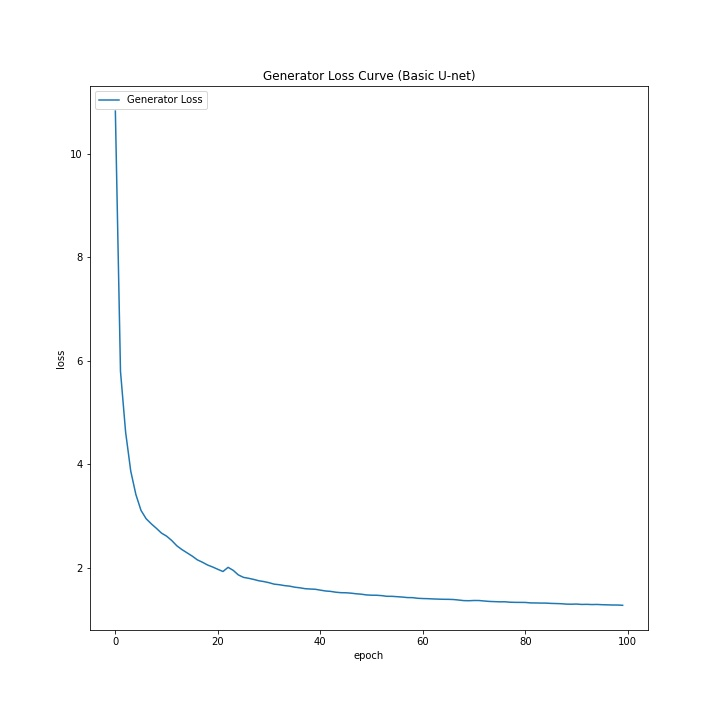
\includegraphics[width=\textwidth]{figures/basic_generator_loss}
		\caption{U-net Generator loss}
		\label{fig: u-net_loss}
	\end{subfigure}
	\begin{subfigure}[b]{0.3\textwidth}
		\centering
		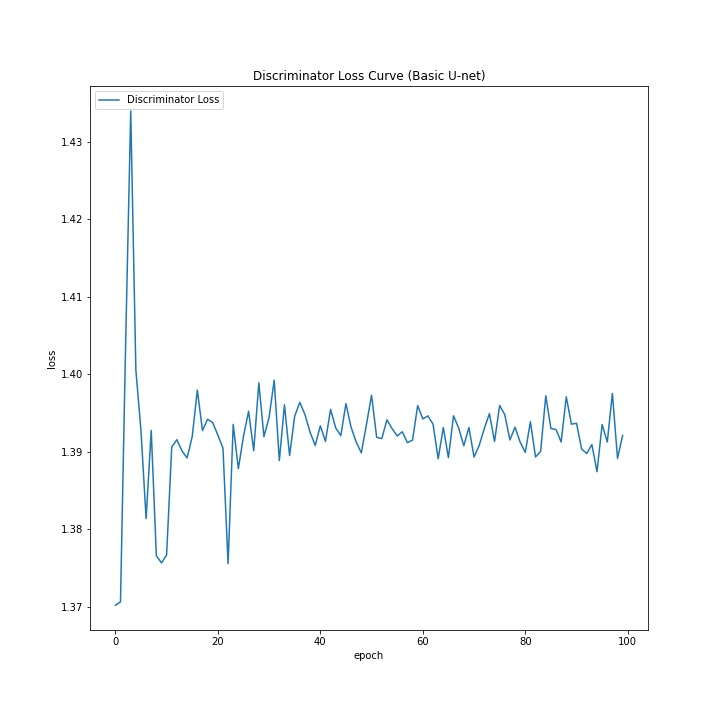
\includegraphics[width=\textwidth]{figures/basic_discriminator_loss}
		\caption{Discriminator loss}
		\label{fig: disc_cus_loss}
	\end{subfigure}
	\caption{Curve plots for Basic U-net \& Custom discriminator}
	\label{fig: basic_unet_curves}
\end{figure}

Figure \ref{fig: u-net_loss} and \ref{fig: disc_cus_loss} shows that the generator converges quite nicely. The discriminator on the other hand oscillates because of the convergence that the generator shows. GAN losses are pretty non-intuitive but we can draw some observations from the loss curves. It seems that the pattern of oscillation and convergence repeats when networks are trained in an adversarial fashion. 

\begin{figure}[!htb]
	\centering
	\begin{subfigure}[b]{0.3\textwidth}
		\centering
		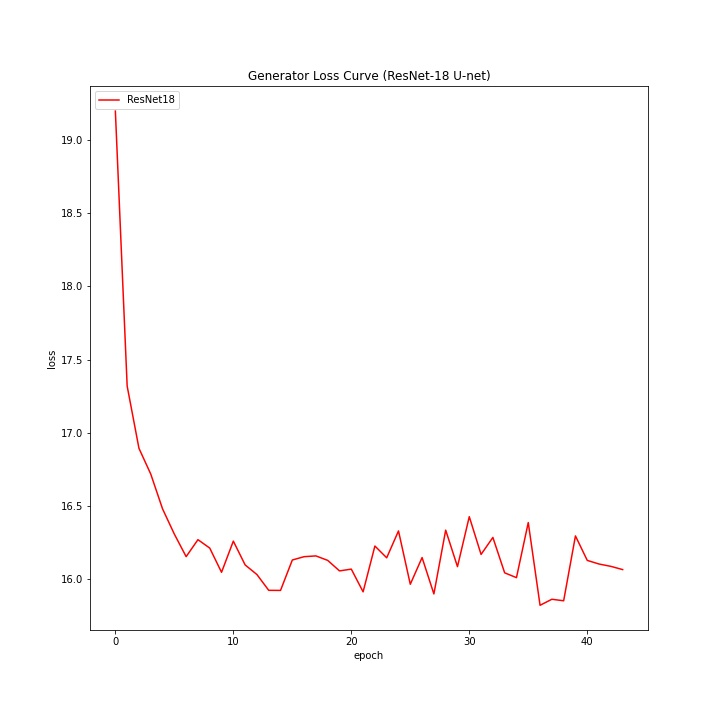
\includegraphics[width=\textwidth]{figures/resnet18_generator_loss}
		\caption{ResNet18 U-net Generator}
		\label{fig: resnet_loss}
	\end{subfigure}
		\hspace{0.1 in}
	\begin{subfigure}[b]{0.3\textwidth}
		\centering
		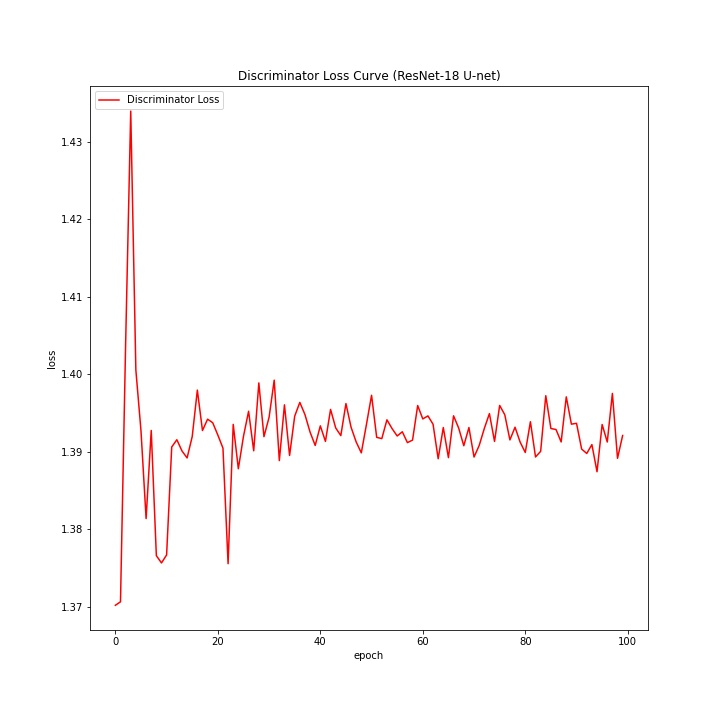
\includegraphics[width=\textwidth]{figures/resnet18_discriminator_loss}
		\caption{ResNet50 discriminator loss}
		\label{fig: resnet50_disc_loss}
	\end{subfigure}
	\caption{Curve plots for ResNet18 U-net \& ResNet50 discriminator}
	\label{fig: resnet18_curves}
\end{figure}

Figure \ref{fig: resnet_loss} and \ref{fig: resnet50_disc_loss} show the same trend repeating even when trained using pre-trained weights with state of the art networks that show excellent results. It is observed that the ResNet U-net with a pre-trained ResNet-18 for its backbone converges decently in the beginning but later shows spikes when nearing the end of training loop. The ResNet50 used as a discriminator shows identical behavior as the custom discriminator above refer fig.\ref{fig: disc_cus_loss}. 

We draw some conclusions based on our understanding of the plots. It seems that the loss convergence doesn't signify whether the model is predicting expected results. The loss function just converges to the minimum value that the cost function descends to, permitted by the learning rate. It would normally signify that the GAN has found some optimum point in the vector space that is at the lowest potential and cant decrease any further. It essentially means that the GAN has leaned enough. Due to the large number of dimensions, owing to the high amount of trainable variables, such combinations, where the function converges, can be huge in volume. Thus, these numbers don't provide any better understanding of the bias or variance the model is facing. Also, we discover that if the loss hasn't converged well, it doesn't necessarily mean that the model hasn't learned anything. On visual inspection, the generated results show similar results to the ground truth, even with high generator losses. This might be due to presence of a content loss parameter in the loss function where we try to minimize the function by  minimizing the L1 norm between the generator predictions and target.

The discriminator shows an increase in the objective loss function in the initial epochs and then settles down in the later phase around an oscillation point. This shows that the discriminator is converging to some permanent number or rather, oscillating around it. We assume this point to be a point of stability between the two networks as the networks are in a constant adversarial battle, meaning if one performs better, the other is bound to perform worse.
\pagebreak
\subsection{Image Colorization}
\hspace*{0.25 in}We present a comparative study of the following models: Basic U-net generator with a custom, residual VGG16 discriminator, hereafter referred to as Basic U-net. A modified U-net with pre-trained ResNet18 as its backbone. We evaluate this model by training it in RGB color space to predict 3 numbers for every pixel and in L*a*b color space where the model predicts the a and b channel alone. We then further train this model to fine-tune it to the task of colorizing astronomical images.

\begin{figure}[!htb]
	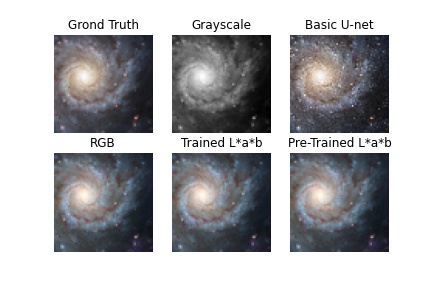
\includegraphics[width=\textwidth]{figures/comparison_color}
	\caption{Results of the colorization study. The first two images in the top row are the ground truth and input image respectively. The next images belong to the output of following, serially: Basic U-net, ResNet18 in RGB colorspace, ResNet18 fine-tuned in L*a*b colorspace, ResNet18 pre-trained U-net in L*a*b colorspace}
	\label{color_results}
\end{figure}

From figure \ref{color_results} we observe that on this particular example, the Basic U-net performs better at predicting results that closely map to the ground truth but the fine-tuned ResNet-18 shows promising results over a larger set of inputs. It can also be observed that the Basic U-net architecture does a decent job of faking the sharpness in the original image and that makes the image appear more realistic as compared to rather blurry outputs from the other networks. 

We also observe that the model trained in the RGB color space performs poorly at predicting values of the three color channels and that results in dominance of one channel (blue in this case) over others. This causes the output, even though reconstructed quite accurately, to have a varied color pattern with high emphasis on one color channel. This might be because of presence of deep layers which cause gradients of certain colors to diminish over time, causing the model to be strongly biased towards the blue color in this case. An increase in the volume of training data and some random pixel shuffling in forward propagation might solve this problem. 

The pre-trained ResNet18 U-net performs decently with the weights gathered by training it over the COCO dataset. The model still lacks the specific coloring intuition in astronomical images and plainly colors specific parts of the images in light colors, leaving majority of the image unaltered. This causes the images to have a slight gray tinge.

Figure \ref{fig: comparisons} shows how the other models perform in different color spaces. We can observe that the Basic U-net model performs good at predicting the outputs but doesn't predict the brightness level of pixels quite accurately. The model seems to be overfitting on the dataset and suffers a high variance on output because there are a lot of testing samples which demonstrate the poor performance of the Basic U-net model as can be seen in figure \ref{fig: u-net_overfit}.

\begin{figure}[!htb]
	\centering
	\begin{subfigure}[b]{0.4\textwidth}
		\centering
		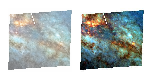
\includegraphics[width=\textwidth]{figures/overfit_1}
		\caption{Sample 2}
		\label{fig: overfit1}
	\end{subfigure}
		\hspace{0.1 in}
	\begin{subfigure}[b]{0.4\textwidth}
		\centering
		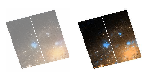
\includegraphics[width=\textwidth]{figures/overfit_2}
		\caption{Sample 2}
		\label{fig: overfit2}
	\end{subfigure}
	\caption{Performance of Basic U-net over samples different from the dataset. The left part is the prediction, right part is the ground truth}
	\label{fig: u-net_overfit}
\end{figure}


\begin{figure}[!htb]
	\centering
	\begin{subfigure}[t]{0.8\textwidth}
		\centering
		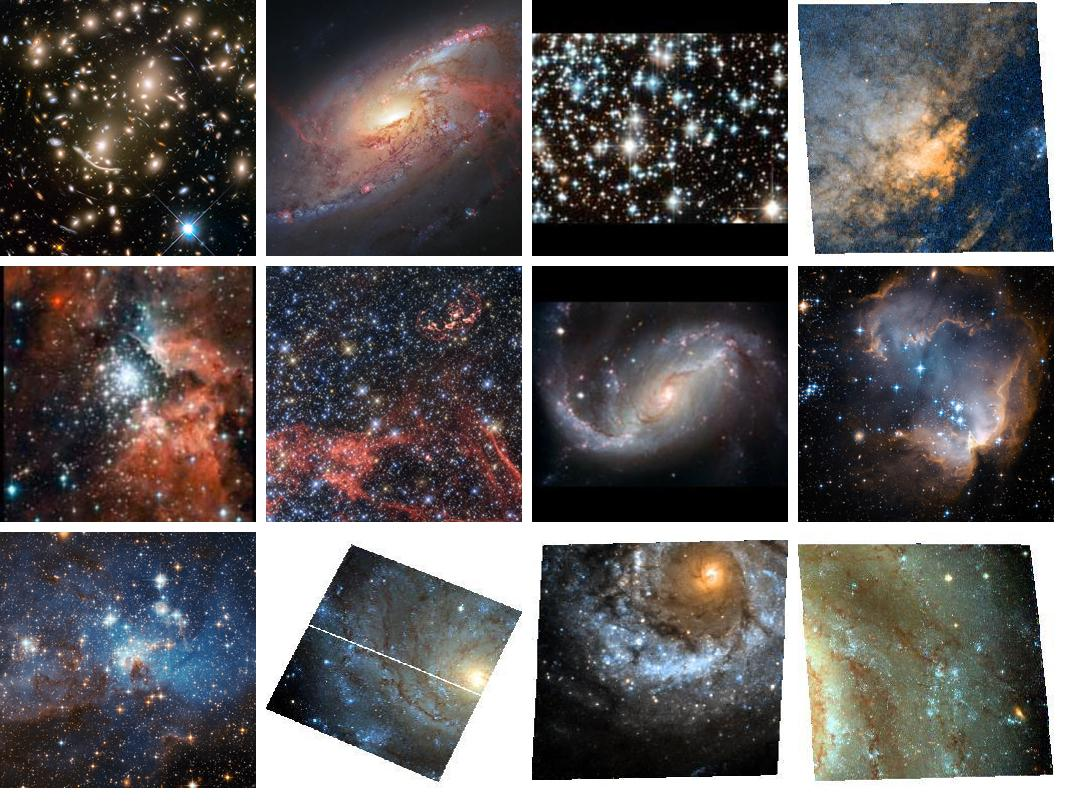
\includegraphics[width=\textwidth]{figures/samples_main}
		\caption{Ground Truth}
		\label{fig: main_color_samples}
	\end{subfigure}
		\hspace{0.1 in}
	\begin{subfigure}[b]{0.8\textwidth}
		\centering
		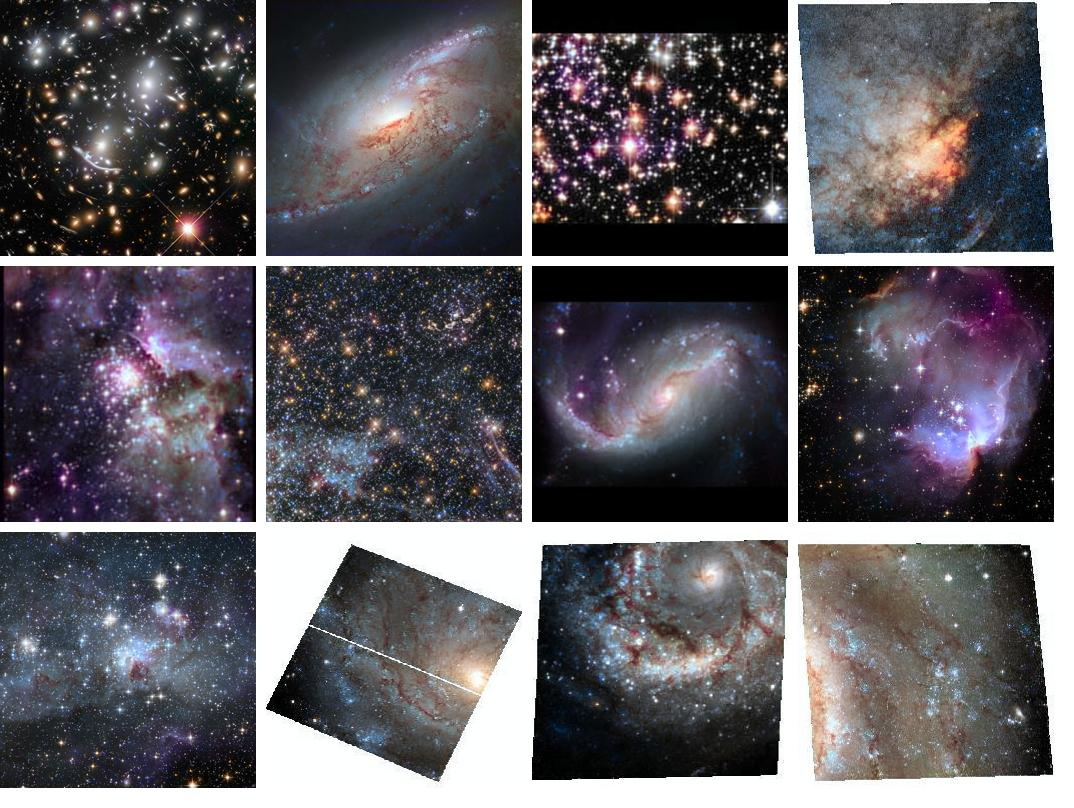
\includegraphics[width=\textwidth]{figures/samples_full-trained}
		\caption{ResNet18 Full trained L*a*b}
		\label{fig: resnet18_full}
	\end{subfigure}
	\caption{Results of fine-tuned ResNet18 in L*a*b colorspace compared with ground truth images}
\end{figure}
\pagebreak
Figure \ref{fig: main_color_samples} shows the ground truth images and figure \ref{fig: resnet18_full} shows the predictions of the ResNet18 full trained model in the L*a*b color space. This model seems to perform best, visually. 
\pagebreak
\begin{figure}[!htb]
	\centering
	\begin{subfigure}[b]{0.5\textwidth}
		\centering
		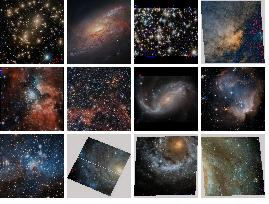
\includegraphics[width=\textwidth]{figures/samples_pix2pix}
		\caption{Basic U-net}
		\label{fig: u-net_samples}
	\end{subfigure}
		
	\begin{subfigure}[b]{0.5\textwidth}
		\centering
		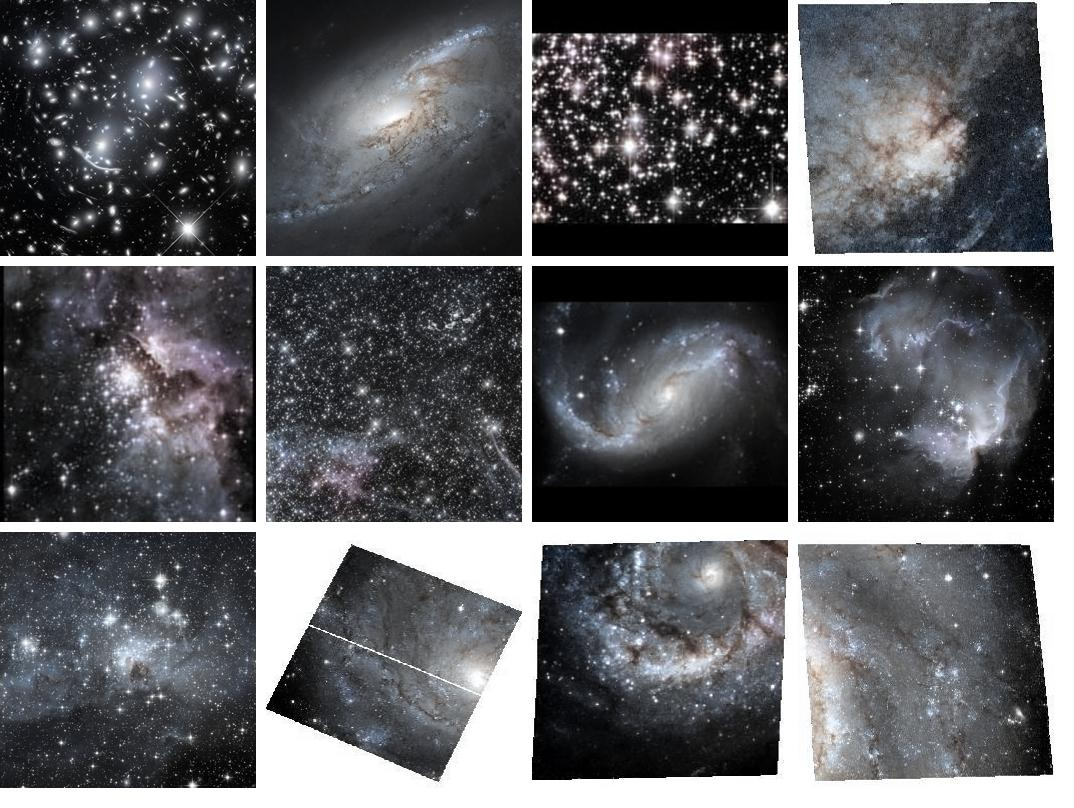
\includegraphics[width=\textwidth]{figures/samples_pre-trained}
		\caption{ResNet18 pre-trained L*a*b}
		\label{fig: resnet18_pre}
	\end{subfigure}
		
	\begin{subfigure}[b]{0.5\textwidth}
		\centering
		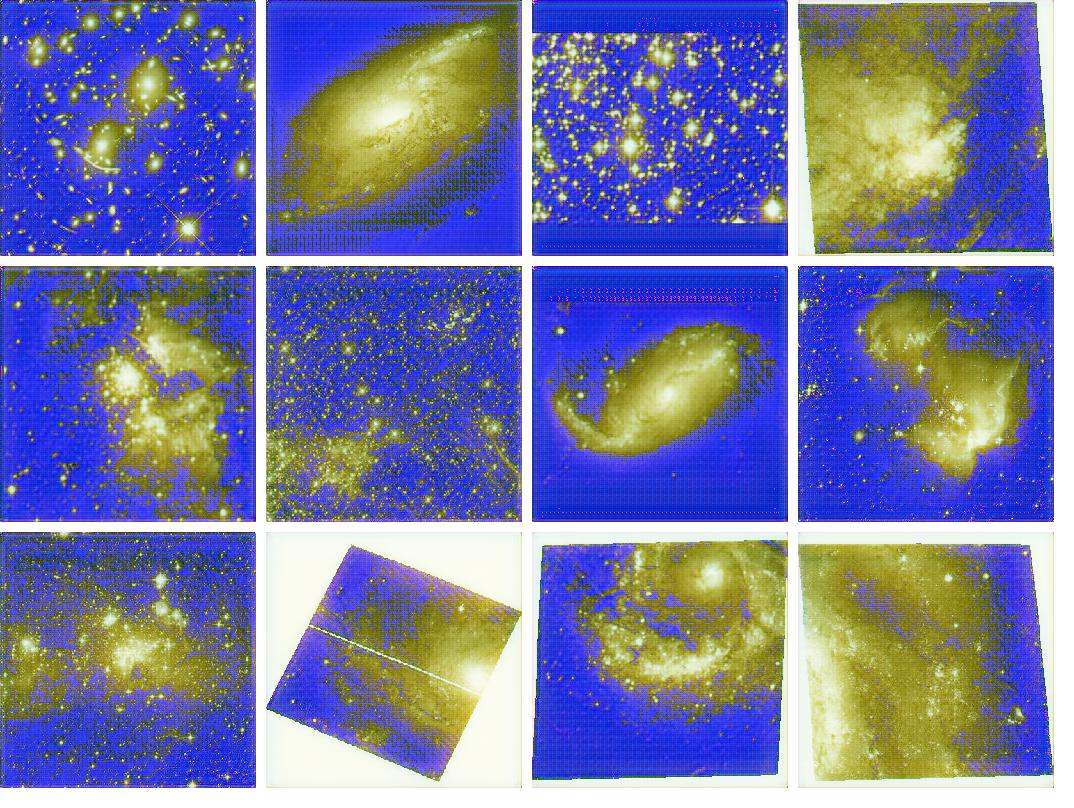
\includegraphics[width=\textwidth]{figures/samples_coco}
		\caption{ResNet18 pre-trained RGB}
		\label{fig: resnet18_rgb}
	\end{subfigure}
	\caption{Results of colorization models (from top to bottom): Basic U-net, ResNet18 U-net pre-trained in L*a*b color space, ResNet18 U-net pre-trained in RGB color space}
	\label{fig: comparisons}
\end{figure}

\pagebreak

To quantitatively estimate the model performance, we measure the L1 and L2 distance between the predictions and the ground truth images in both RGB as well as L*a*b colorspace. 

\begin{table}[!htb]
\centering
\setlength{\tabcolsep}{10pt} % Default value: 6pt
\renewcommand{\arraystretch}{1.5} % Default value: 1
\begin{tabular}{c | c | c | c}
        \hline
        \textbf{Model} & \textbf{Color Space} & \textbf{
        L1 Distance} & \textbf{L2 Distance}\\
        \hline
        ResNet-18 (Pre-trained) & L*a*b & 64.5409 & 2.77\\
        ResNet-18 (Fine-tuned) & L*a*b & 65.1119 & 2.62\\
        ResNet-18 (Pre-trained) & RGB & 125.5554 & 9.04\\
        U-net & RGB & 77.3273 & 3.986\\
        \hline
    \end{tabular}
\caption{Colorization: Average per-pixel L1 \& L2 distance between generated images and ground truth}
\label{tab:colorization_results}
\end{table}

Table \ref{color_results} shows that the RGB color space performs poorly on the task of colorization. In terms of the L1 distance, the best performance is achieved on the ResNet18 U-net with pre-trained weights. This goes to prove the unreliability of distance metrics in model performance evaluation. The model, although quantitatively, performs better than the fine-tuned model but in reality, fails to produce images that might be visually appealing. The L2 distance metric shows how the fine-tuned model might, in reality, be fitting slightly better over the data to predict correct color combination as its output. We still consider the results from the fine tuned model to be better than the other performing models and further investigate the per-channel predictions by the model.

\begin{table}[!htb]
\centering
\setlength{\tabcolsep}{4pt} % Default value: 6pt
\renewcommand{\arraystretch}{1.5} % Default value: 1
    \begin{tabular}{c | c | c | c}
        \hline
        \textbf{Distance} & \textbf{Red} & \textbf{
        Green} & \textbf{Blue}\\
        \hline
        L1 Norm & 64.6078 & 38.5994 & 92.1283\\
        L2 Norm & 3.4531 & 1.0253 & 3.8046\\
        \hline
    \end{tabular}
\caption{Channel wise averages of ResNet-18 finetuned network}
\label{tab:channel_wise_results}
\end{table}

Table \ref{tab:channel_wise_results} shows the RGB channel averages of the outputs produced by the fine tuned model. It can be observed that the feature embeddings produced by the model in *a, *b color spaces maps to the green channel with the least error. This might be indicative that the model is performing poorly on images that have a high content of red-blue colors. 

To further evaluate the actual outputs produced in the L*a*b color space, we compare the *a, *b channels of the ResNet18 architectures. 

\begin{table}[!htb]
\centering
\setlength{\tabcolsep}{3pt} % Default value: 6pt
\renewcommand{\arraystretch}{0.9} % Default value: 1
    \begin{tabular}{c | c c | c c}
        \hline
        \hline
        \multirow{2}{*}{\footnotesize{Model}} & 
            \multicolumn{2}{c|}{\footnotesize{L1 Distance}} & \multicolumn{2}{c}{\footnotesize{L2 Distance}}\\
                & \footnotesize{a} & \footnotesize{b} & \footnotesize{a} & \footnotesize{b}\\
        \hline
        \footnotesize{ResNet-18 (Pre-trained)}  & \footnotesize{0.00588} &  \footnotesize{0.00501} & \footnotesize{0.01565} & \footnotesize{0.03208}\\
        \footnotesize{ResNet-18 (Fine-tuned)} & \footnotesize{0.00257} & \footnotesize{0.00727} & \footnotesize{0.01721} & \footnotesize{0.03316}\\
        \hline
    \end{tabular}
\caption{L1 \& L2 channel wise distances in L*a*b colorspace}
\label{tab:lab_color_results}
\end{table} 
In table \ref{tab:lab_color_results}, L1 distance, we can see the performance of fine-tuned model to be better in channel *a but poor in *b compared to the pre-trained model. The L2 distance metric rules out the possibility of the fine-tuned model performing better than the pre-trained model. In reality, the fine-tuned model is orders of magnitude better at predicting output abstractions with the L channel as its input, thus contradicting the quantitative results.

\subsection{Image Super Resolution}
\hspace*{0.25 in}We implement the basic SR-GAN proposed by Ledig and train it to improve super-resolution task. We compare the trained model with pre-trained SRGAN model, EDSR-GAN proposed by \cite{lim2017enhanced} and WDSR-GAN proposed by \cite{yu2018wide}.

\begin{figure}[!htb]
	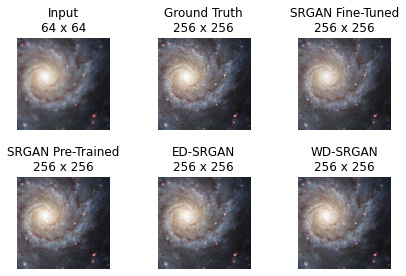
\includegraphics[width=0.8\textwidth]{figures/comparison_upscale}
	\caption{Results of the super-resolving models. The first two images in the top row are the input image and ground truth respectively. The next images belong to the output of following, serially: Fine-tuned SRGAN, pre-trained SRGAN, EDSR, WDSR}
	\label{fig: sr_results}
\end{figure}

Figure \ref{fig: sr_results} shows how the networks perform on the task of predicting pixels while upscaling of the image. All the networks perform really well and its difficult to distinguish the outputs visually. It may be observed that the fine-tuned network produces images that look slightly better than the other counter-parts. The best performing network seems to be the WDSR-GAN with a very little error in predicting the output. 

\begin{figure}[!htb]
	\centering
	\begin{subfigure}[b]{0.8\textwidth}
		\centering
		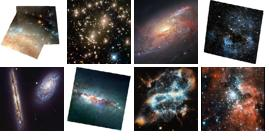
\includegraphics[width=\textwidth]{figures/inputsamples_superR}
		\caption{Input Distribution}
		\label{fig: sr_input_samples}
	\end{subfigure}
		
	\begin{subfigure}[b]{0.8\textwidth}
		\centering
		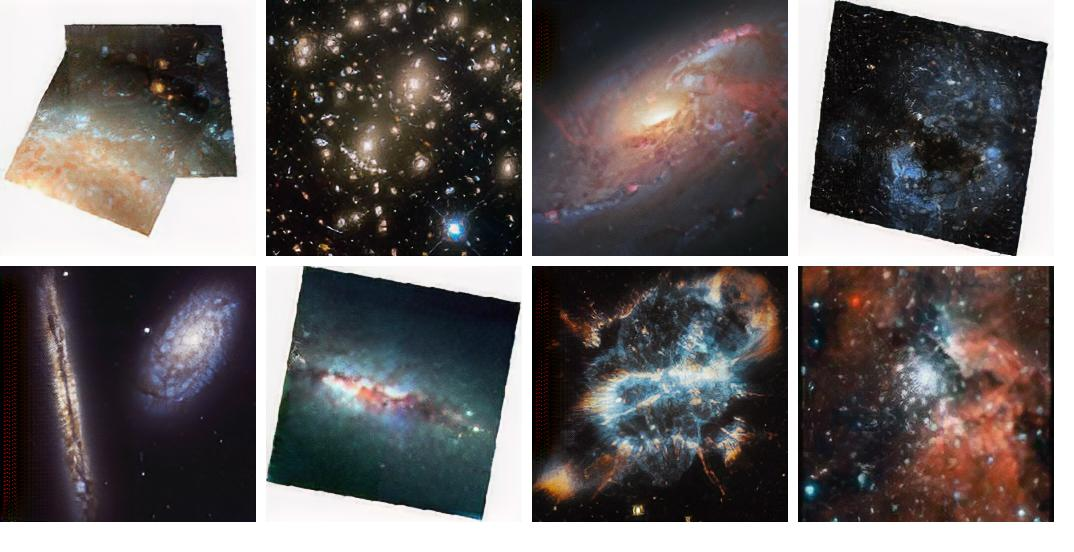
\includegraphics[width=\textwidth]{figures/samples_SRGAN}
		\caption{SRGAN fine-tuned output}
		\label{fig: sr__outputs}
	\end{subfigure}
	\caption{Results of SRGAN. \ref{fig: sr_input_samples} shows the input data and \ref{fig: sr__outputs} shows the corresponding output}
	\label{fig: sr_comparisons}
\end{figure}

It is evident that the model produces acceptable results on visual inspection. The main reason behind this might, again, be the random pixel shuffling between every upscaling pass. 

As opposed to colorization, super-resolution needs a quantitative estimation to determine which model performs best among the give models. 

\begin{table}[!htb]
\centering
\setlength{\tabcolsep}{10pt} % Default value: 6pt
\renewcommand{\arraystretch}{0.9} % Default value: 1
    \begin{tabular}{c | c | c }
        \hline
        \hline
        \footnotesize{\textbf{Model}} & \footnotesize{\textbf{
        L1 Distance}} & \footnotesize{\textbf{L2 Distance}}\\
        \hline
        \footnotesize{Ledig SRGAN (Fine-tuned)} & \footnotesize{87.1090} & \footnotesize{3.754}\\
        \footnotesize{Ledig SRGAN (Pre-trained)} & \footnotesize{114.8043} & \footnotesize{5.953}\\
        \footnotesize{ED-SRGAN} & \footnotesize{80.9414} & \footnotesize{3.684}\\
        \footnotesize{WD-SRGAN} & \footnotesize{79.7262} & \footnotesize{3.627}\\
        \hline
    \end{tabular}
\caption{Super-Resolution: Per-pixel Average L1 \& L2 distance between generated images and ground truth}
\label{tab:Super-resolution_results}
\end{table}

\pagebreak
Table \ref{tab:Super-resolution_results} shows the L1 and L2 distances of predicted results by each model with the ground truth image. It is observed that Ledig's SRGAN, after a bit of fine-tuning performs really well in comparison to the the pre-trained version. To further improve this, \cite{lim2017enhanced} proposed an optimized version of SRGAN by removing the unnecessary modules in the conventional resnets and showed that Enhanced Deep Residual Networks performed better at upscaling task. When trained in an adversarial manner, the ED-SRGAN performs better than the traditional SRGAN. \cite{yu2018wide} further improved the idea by increasing the widening factor ($\times 2$ and $\times 4$) to ($\times 6$ and $\times 9$). This Wide Activation Deep Super Resolution network further improved the performance for single image super-resolution. When we implement this in an adversarial manner, we achieve excellent results. It is evident from the results that the best performing network is the WDSR.

\chapter{Summary and Conclusion}
\section{Summary and Conclusion}
\hspace*{0.25 in}The project mainly tackles the problem of colorizing astronomical images and super-resolving them for astronomical inspection. We explore various methodologies proposed till date that efficient colorize and super-scale images with results that are significantly closer to the ground truth distribution. We scrape the data from Hubble Legacy Archive, Hubble Main website and Hubble Heritage project and created a filtered and clean dataset of 4700 images. We split the data and use 500 images, roughly 10\% of the data for testing purposes. To compensate for the lack of data, we implement several pre-trained architectures and fine-tune their abstractions over our dataset to find the most effective solution.\\
\hspace*{0.25 in}For the colorizing model, we explore usage of U-net architectures starting from a basic U-net model and experiment with different color spaces and empirically confirm the superiority of L*a*b color space in image colorization problem. We use the state of the art ResNet-18 to provide as a backbone of the encoder and build a U-net around it. The pre-trained network over COCO dataset in RGB colorspace produces significantly weaker results as compared to the subsequent network in L*a*b colorspace. The best performing model turns out to be the ResNet18 U-net which is fine-tuned over our particular dataset to produce appealing and similar results to the ground truth.\\
\hspace*{0.25 in}The Super-resolution model is based largely on the SRGAN proposed by \cite{ledig2017photorealistic}. We use the generator weights and sample results from the training set to inspect the results. It is found that the model performs really well on the pre-trained weights and we decide to fine-tune it to our application. After fine-tuning the model, we train other state of the art single image super-resolution models such as EDSR \citep{lim2017enhanced} and WDSR \citep{yu2018wide}. These provide further insights into the problem and simultaneously, improve the results.\\
\hspace*{0.25 in}While studying and improving the performance of these models, we explore performance metrics of GANs and evaluation methodologies implemented to test out conditional GANs. It is evident that the loss curves of generator and discriminator do not provide us with any intuition about the model performance. We also discover that standard distance metrics cannot be used to evaluate GANs and quantitative methods that exist to evaluate GANs are unreliable. We prove so by contradiction of qualitative samples and quantitative measurements of the best performing architecture for colorization models. However, we observe that quantitative estimation is quite reliable for the problem of single image super-resolution and can be helped to determine which model is better suited for the task.

\section{Future Scope}
\hspace*{0.25 in}Though we obtain moderately good results, a vast amount of algorithms still remain unscratched. A more powerful model such as SE-ResNext, EfficientNet and more state-of-the-art models can be implemented and trained over millions of images from the Imagenet. With even more hardware resources and availability of data, we can explore computationally heavy models for a better approximation. An image stitching algorithm can be applied on the produced images to generate large scale astronomical images for scientific study. Colorization can be improved by the virtue of exploring different loss functions using weighted losses to reduce loss problem for low saturation regions. We can introduce a gradient penalty for the SRGAN architecture and include the WGAN \citep{arjovsky2017wasserstein} which will stabilize the discriminator to stay within the space of 1-Lipschitz function. Progressively growing GANs \citep{karras2018progressive} can be applied so that the dimensions can be further improved with more stability and greater sharpness.

\section{Applications}
\hspace*{0.25 in}The images are upscaled and colourized using a completely automated algorithm which uses Deep Learning. Generative Adversarial Networks are  successfully used for the implementation. The algorithm can directly be applied for creating images that can be studied by astronomers. It is anticipated that this will aid the astronomers vastly in their efforts.

\bibliographystyle{dcu}
\bibliography{biblo}


\begin{appendices}

\chapter{Plagiarism Report }


\begin{figure}
	\centering
    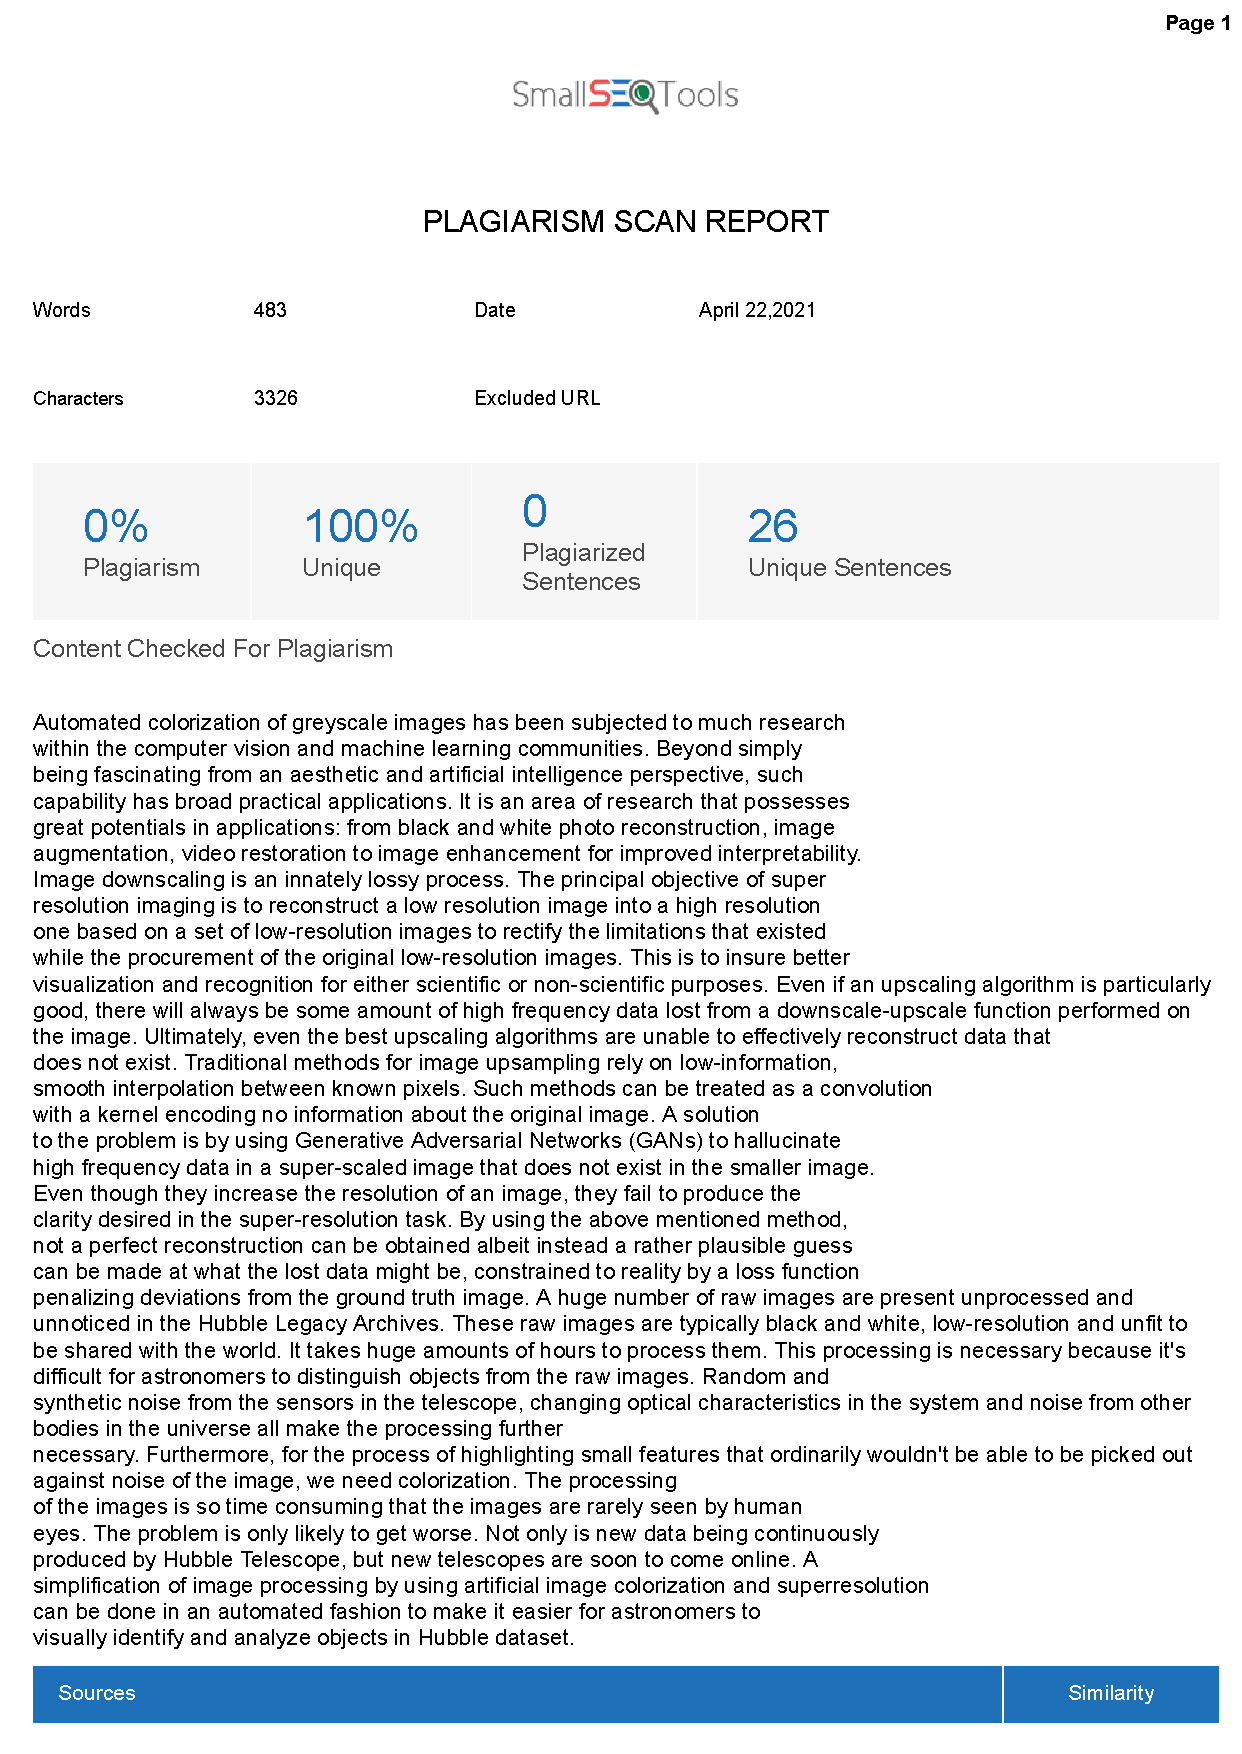
\includegraphics[scale=0.7]{plagiarism/abstract.pdf}
    \caption{Plagiarism report for Abstract}
    \label{PlagiarismAbstract}
\end{figure}

\begin{figure}
	\begin{subfigure}[H]{\textwidth}
		\centering
    	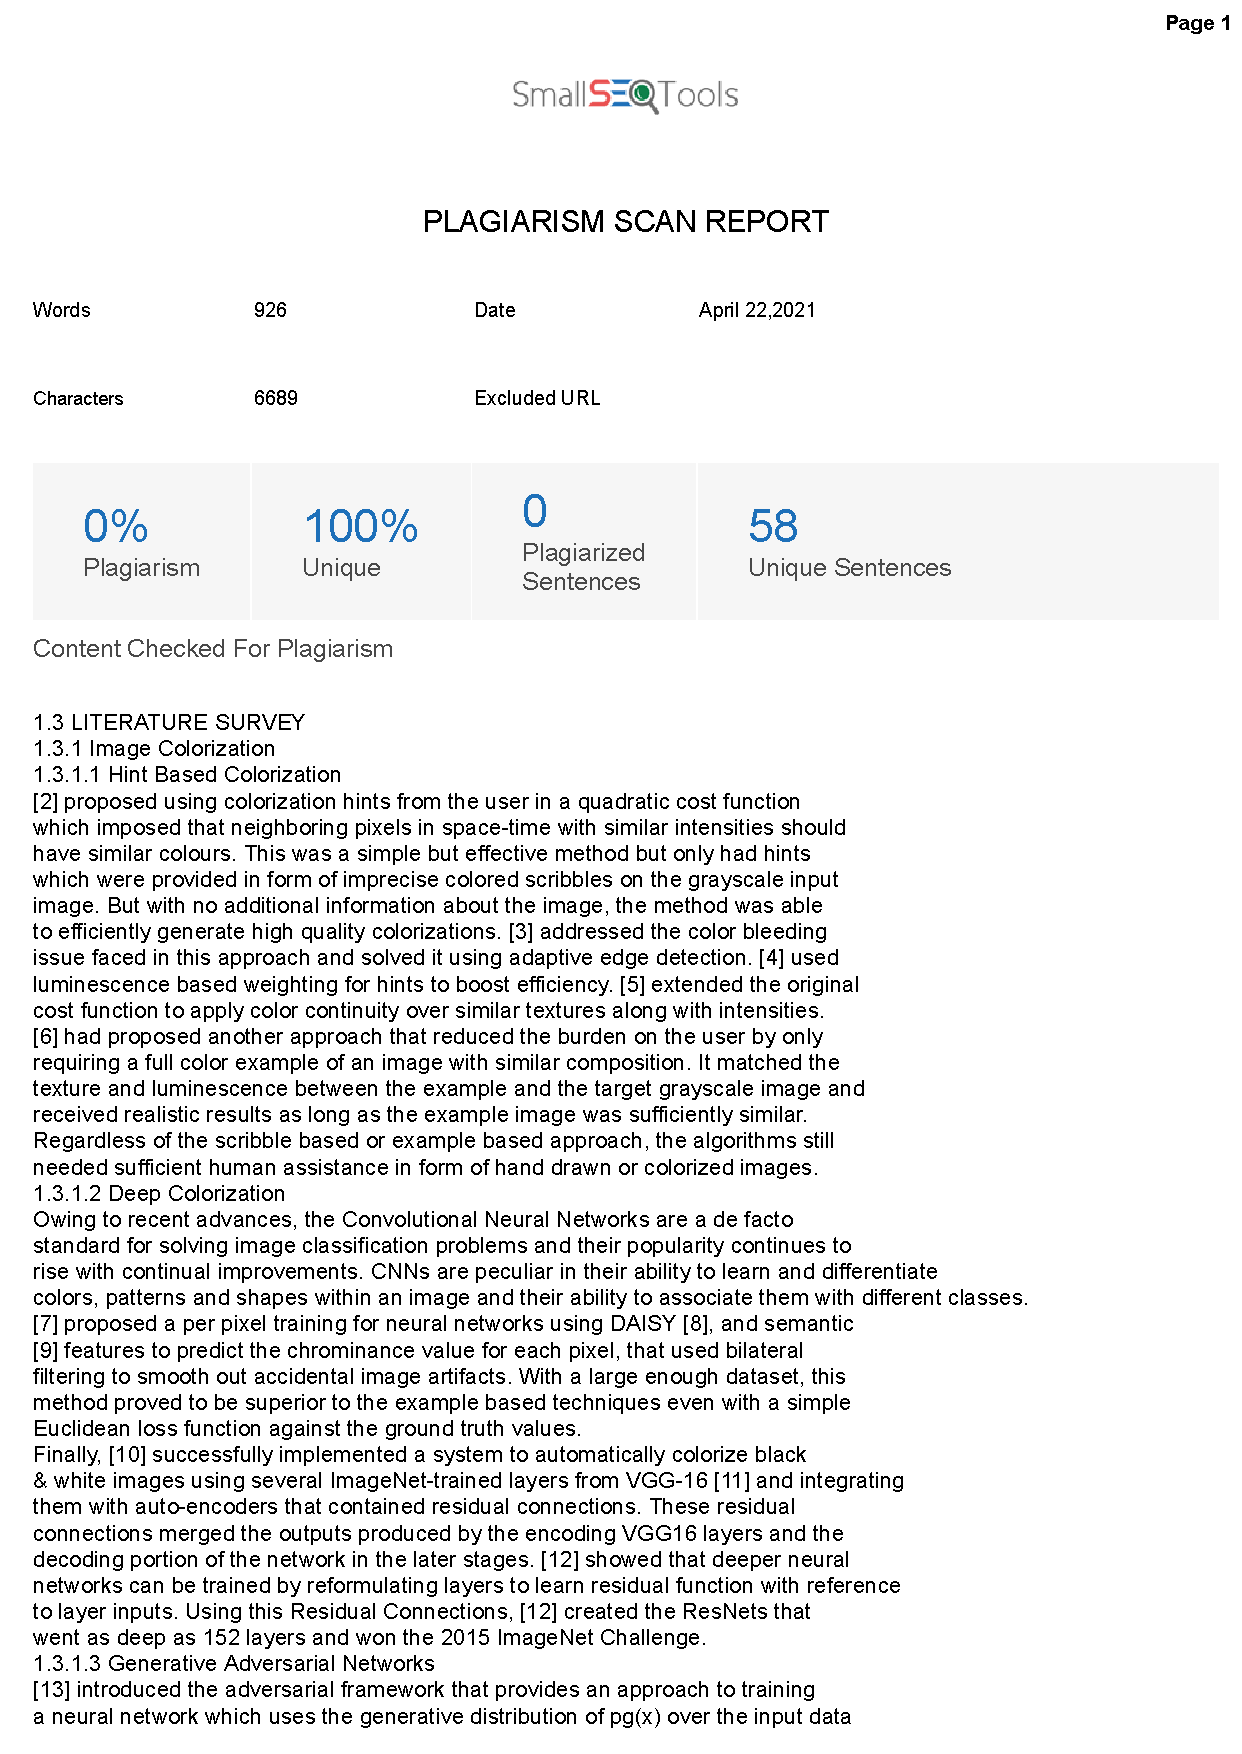
\includegraphics[scale=0.7, page=1]{plagiarism/literature_survey.pdf}
    \end{subfigure}
 \caption{Plagiarism report for Literature Review}
    \label{PlagiarismLitSurvey1}
\end{figure}
\begin{figure}\ContinuedFloat
    \begin{subfigure}[H]{\textwidth}
    	\centering
    	\includegraphics[scale=0.7, page=2]{plagiarism/literature_survey.pdf}
    \end{subfigure}
    \caption{Plagiarism report for Literature Review (contd.)}
    \label{PlagiarismLitSurvey2}
\end{figure}

\begin{figure}
	\begin{subfigure}[H]{\textwidth}
		\centering
    	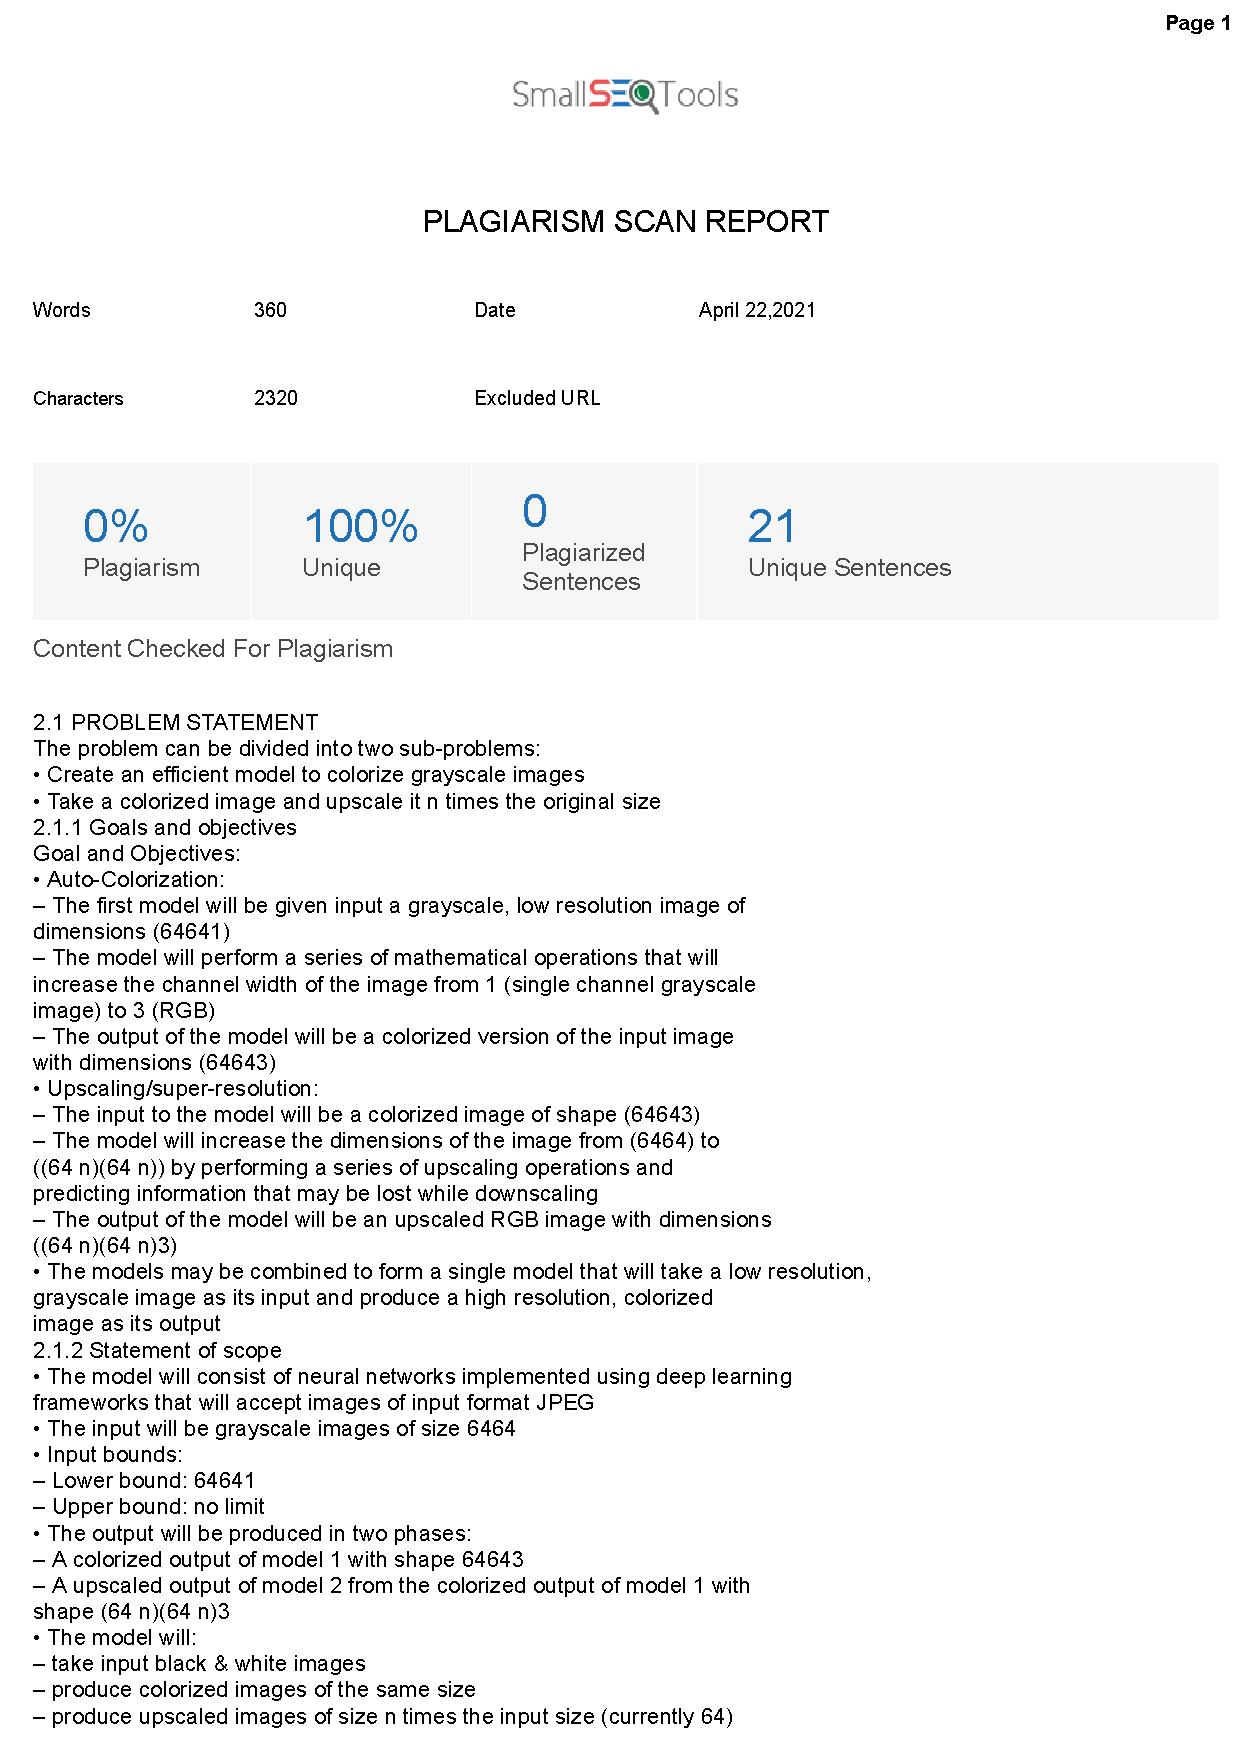
\includegraphics[scale=0.7, page=1]{plagiarism/problem_definition&scope_1.pdf}
    \end{subfigure}
 \caption{Plagiarism report for Problem Definition and Scope (Part 1)}
    \label{PlagiarismPDS1}
\end{figure}
\begin{figure}\ContinuedFloat
    \begin{subfigure}[H]{\textwidth}
    	\centering
    	\includegraphics[scale=0.7, page=2]{plagiarism/problem_definition&scope_1.pdf}
    \end{subfigure}
    \caption{Plagiarism report for Problem Definition and Scope (Part 1) (contd.)}
    \label{PlagiarismPDS1_2}
\end{figure}

\begin{figure}
	\begin{subfigure}[H]{\textwidth}
		\centering
    	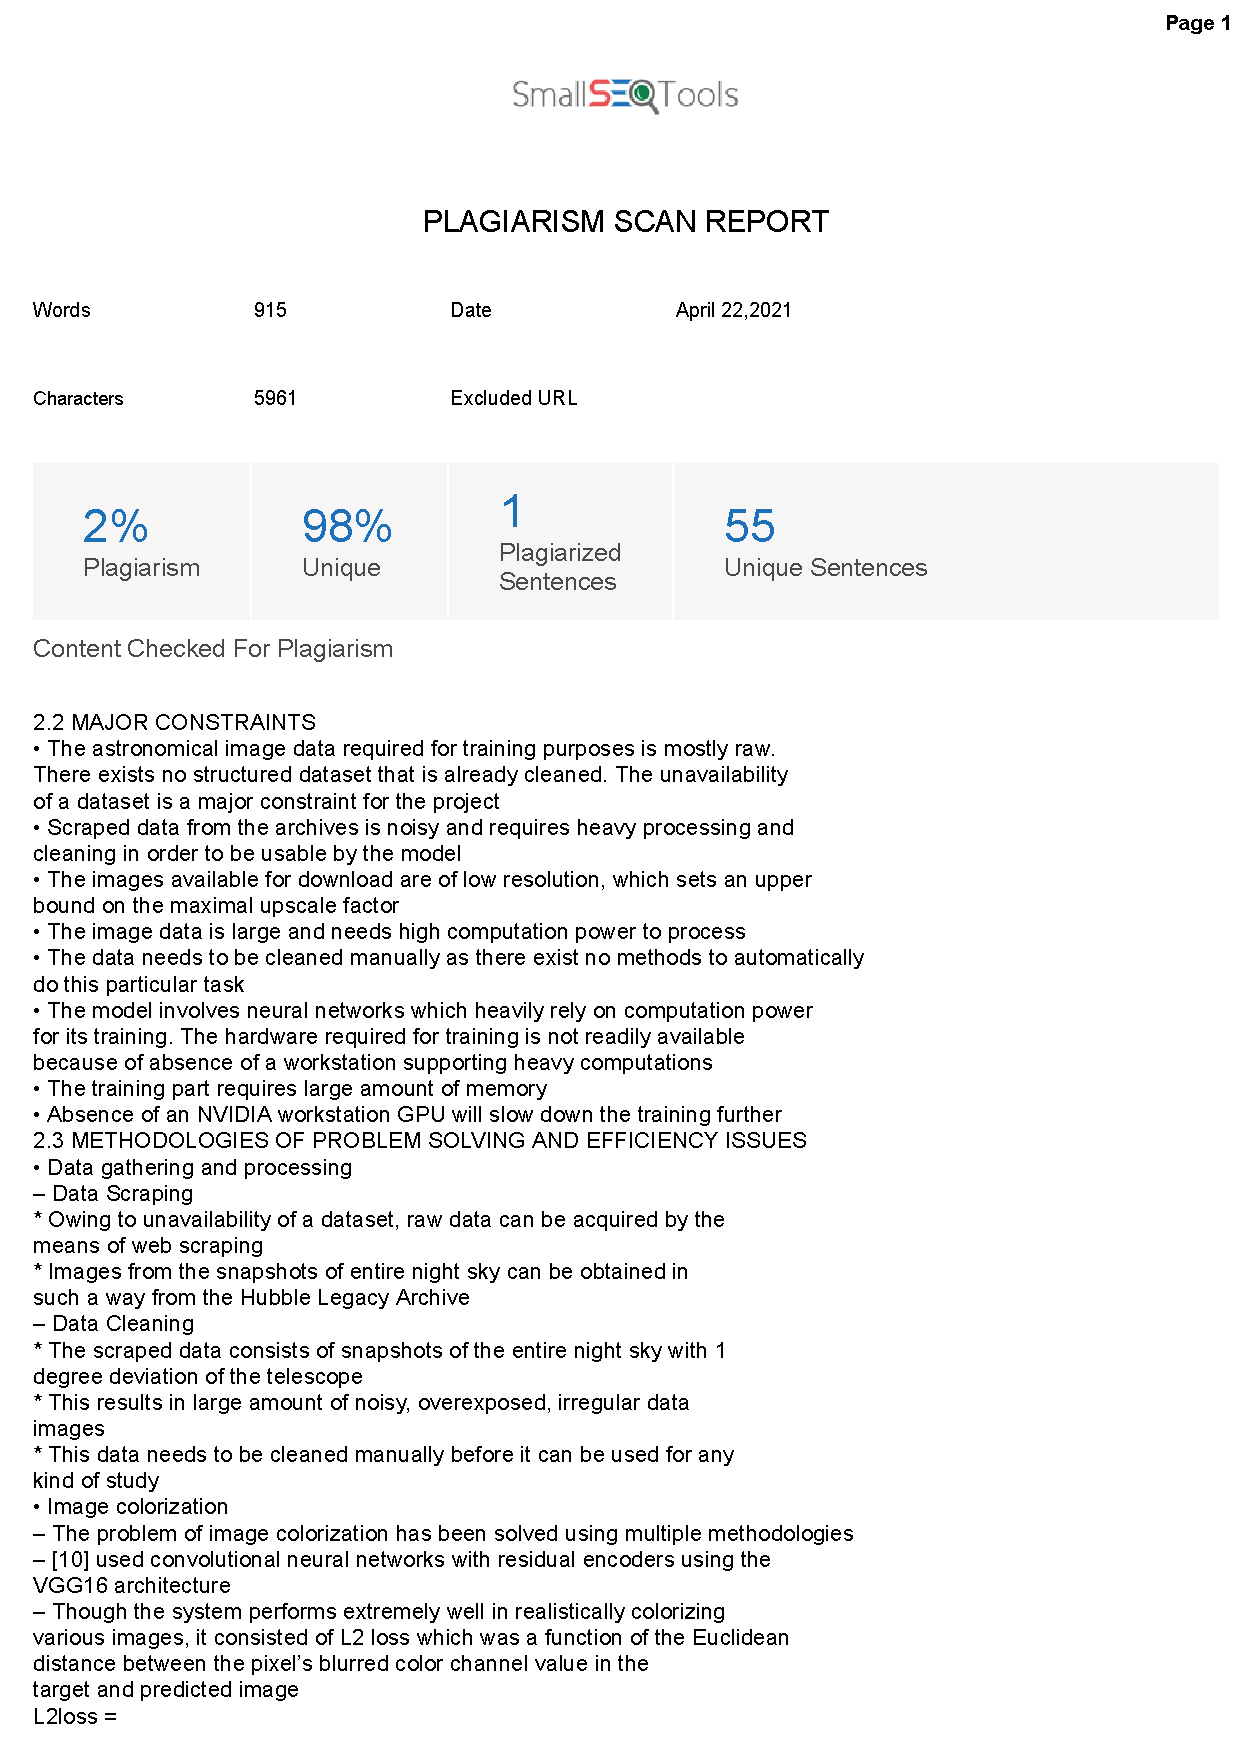
\includegraphics[scale=0.7, page=1]{plagiarism/problem_definition&scope_2.pdf}
    \end{subfigure}
 \caption{Plagiarism report for Problem Definition and Scope (Part 2)}
    \label{PlagiarismPDS2}
\end{figure}
\begin{figure}\ContinuedFloat
    \begin{subfigure}[H]{\textwidth}
    	\centering
    	\includegraphics[scale=0.7, page=2]{plagiarism/problem_definition&scope_2.pdf}
    \end{subfigure}
    \caption{Plagiarism report for Problem Definition and Scope (Part 2) (contd.)}
    \label{PlagiarismPDS2_2}
\end{figure}

\begin{figure}
	\begin{subfigure}[H]{\textwidth}
		\centering
    	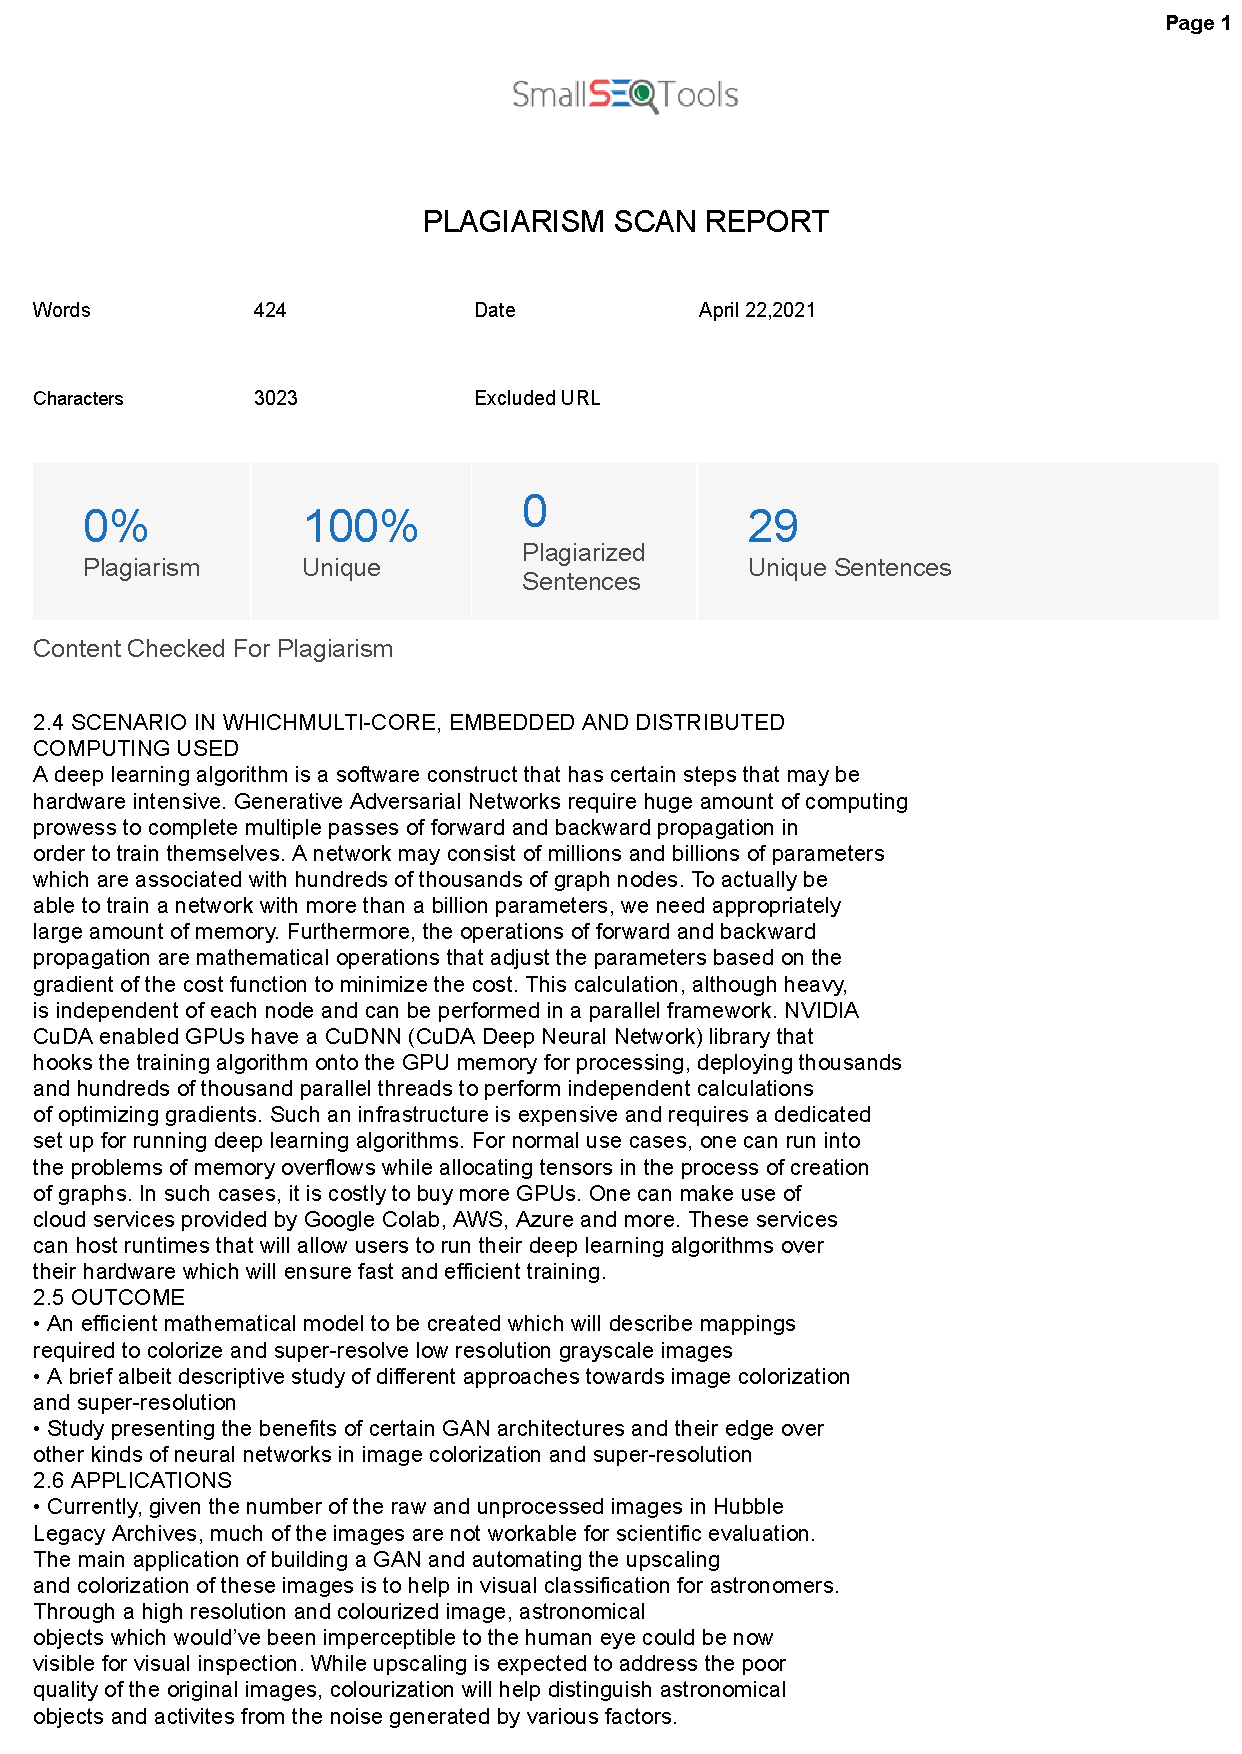
\includegraphics[scale=0.7, page=1]{plagiarism/problem_definition&scope_3.pdf}
    \end{subfigure}
 \caption{Plagiarism report for Problem Definition and Scope (Part 3)}
    \label{PlagiarismPDS3}
\end{figure}

\begin{figure}
	\centering
    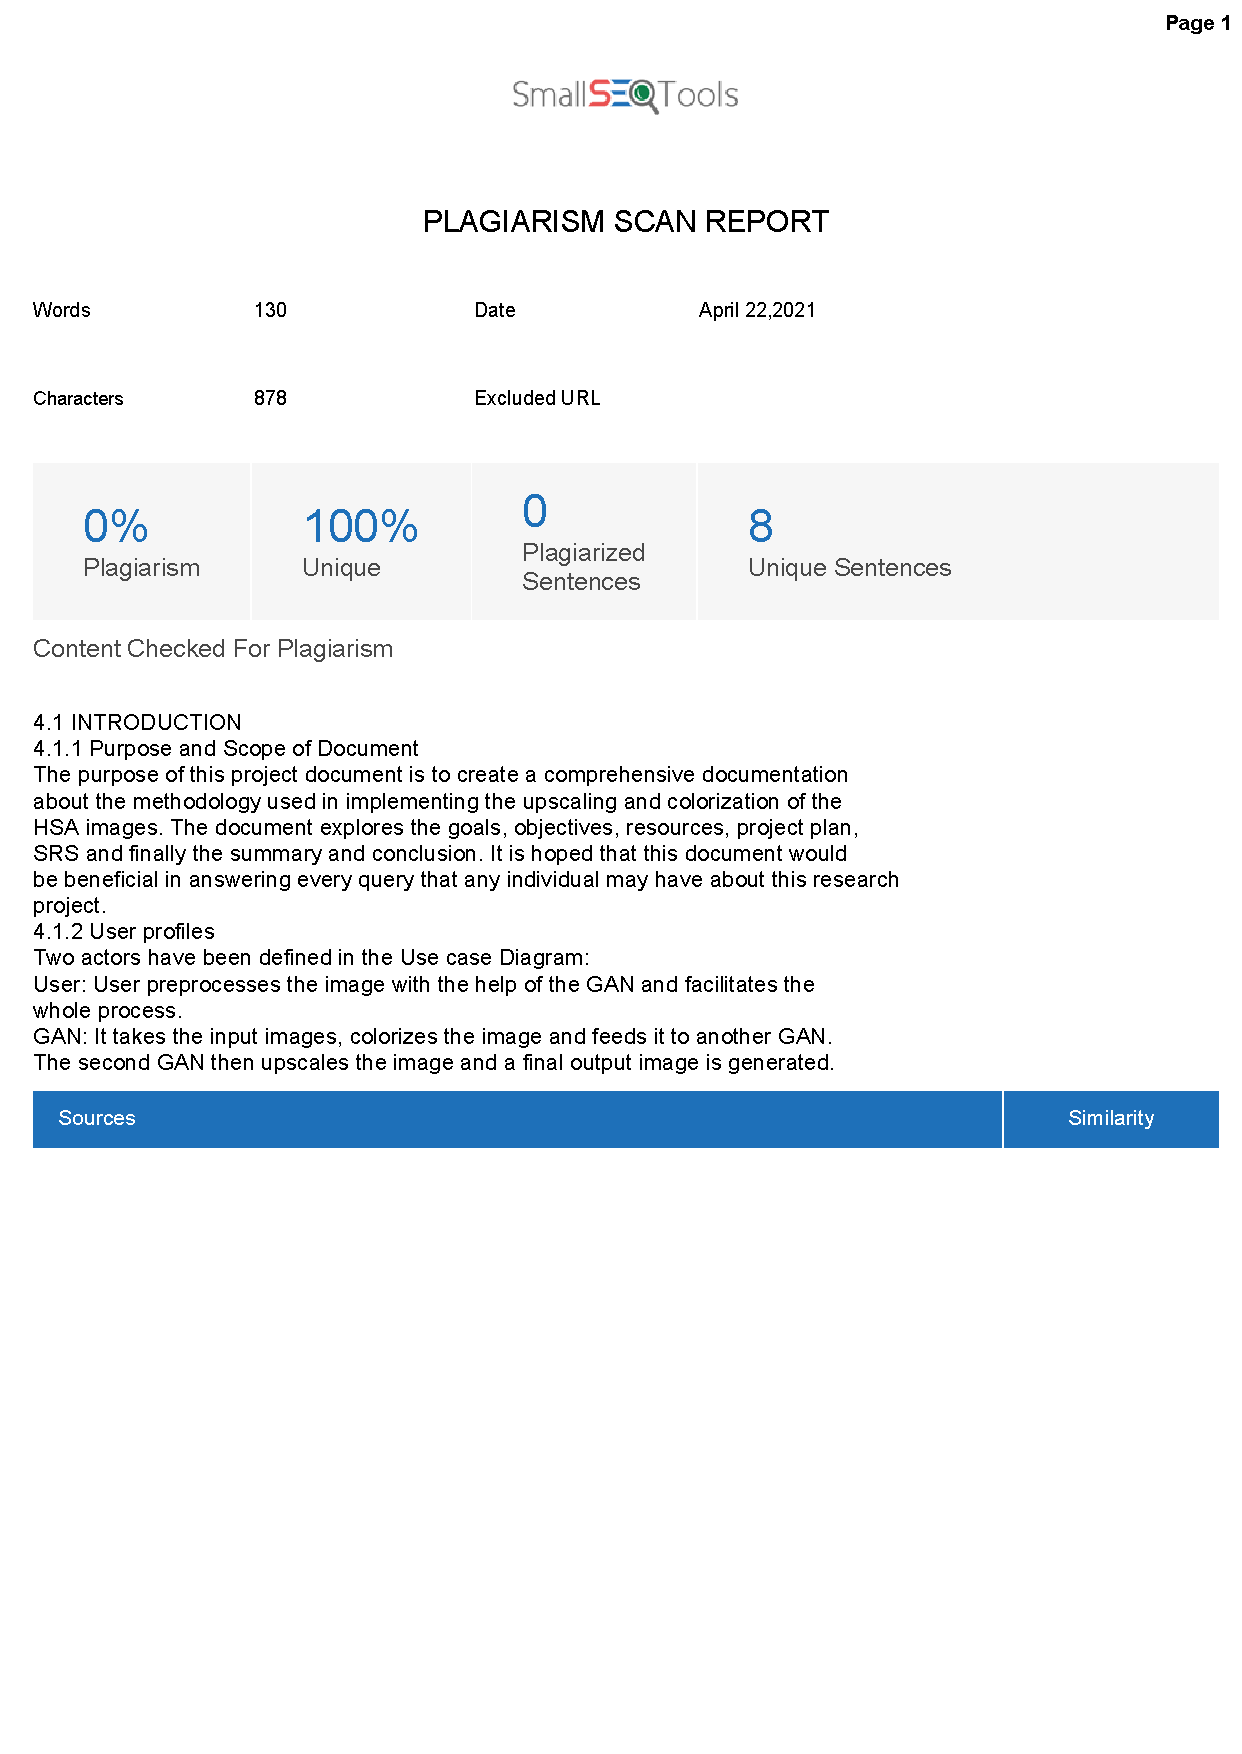
\includegraphics[width=\textwidth, height=\textheight]{plagiarism/software_requirement_specification.pdf}
    \caption{Plagiarism report for Software Requirement Specifications}
    \label{PlagiarismSRS}
\end{figure}

\begin{figure}
	\begin{subfigure}[H]{\textwidth}
		\centering
    	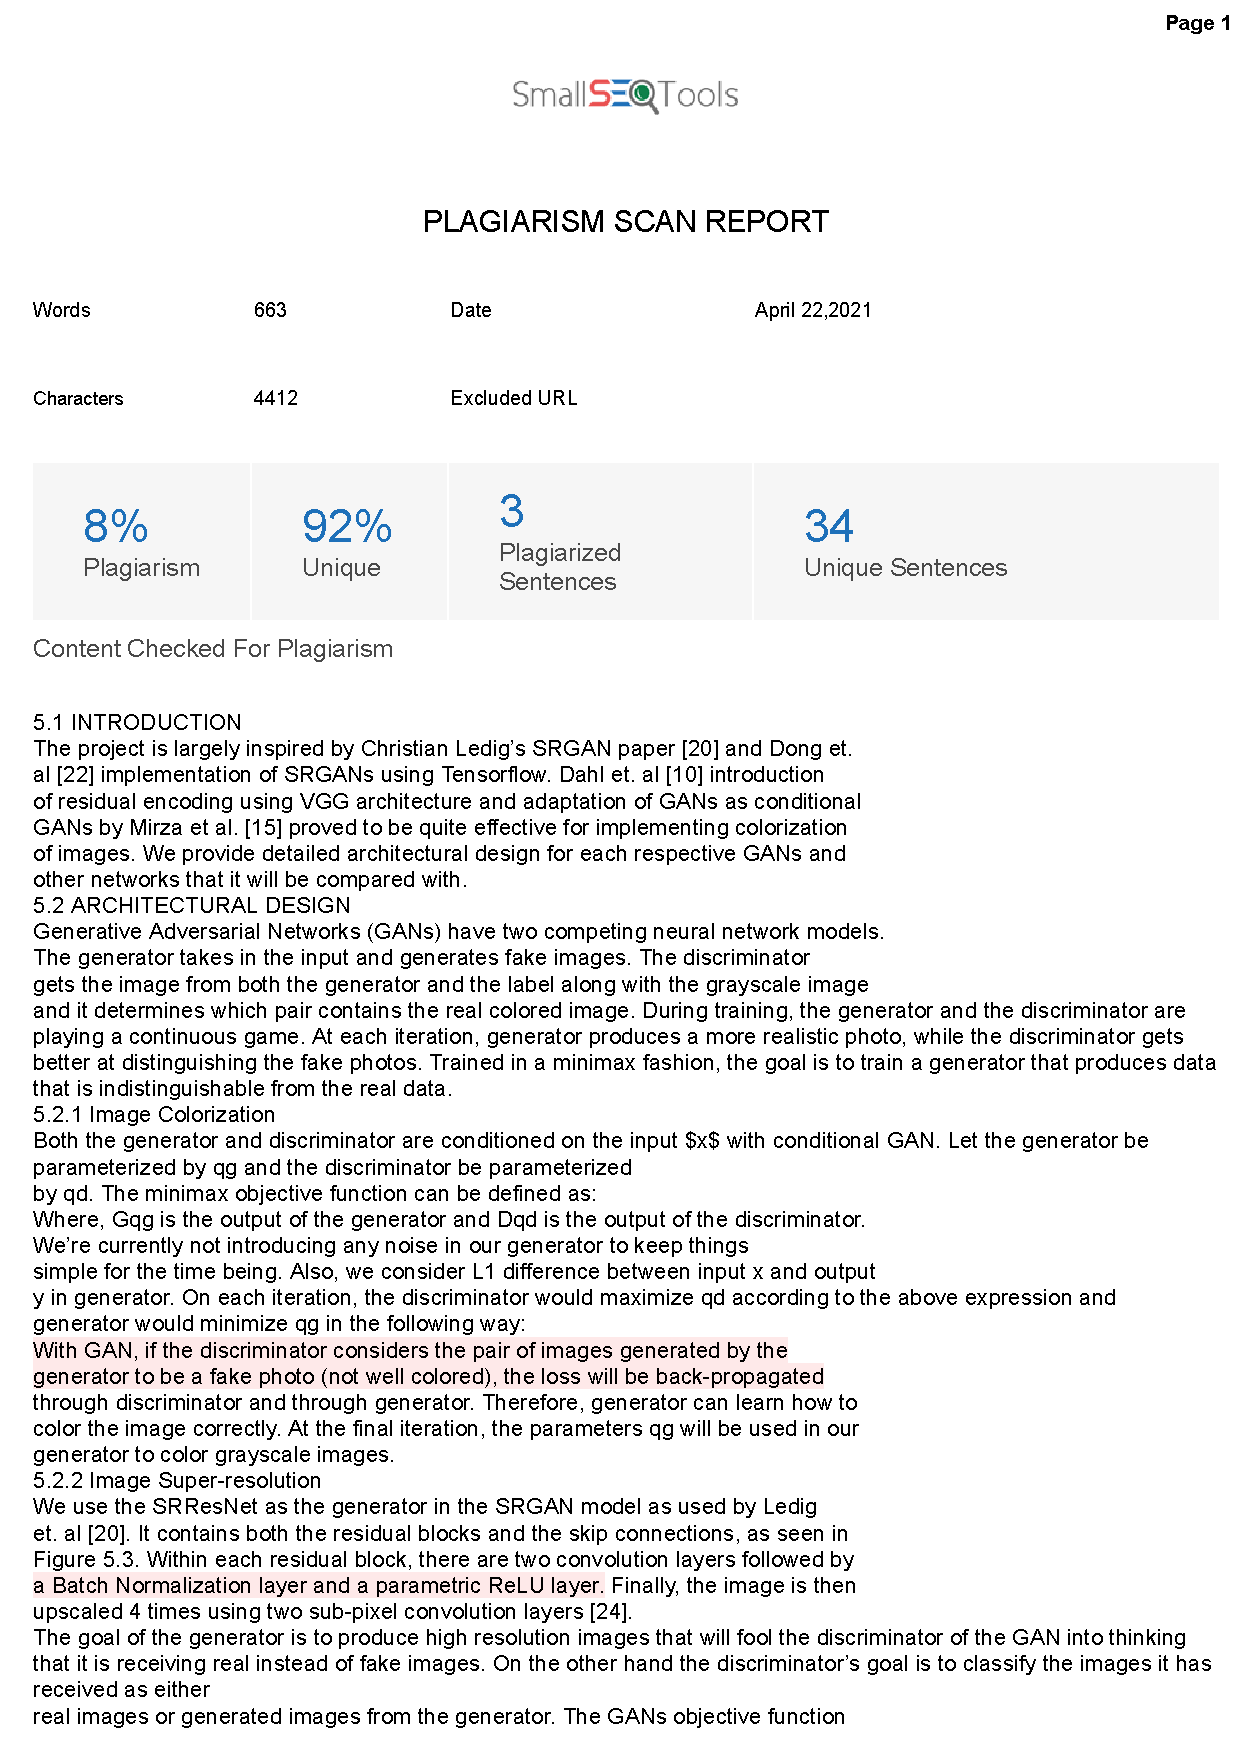
\includegraphics[scale=0.7, page=1]{plagiarism/detailed_design_documentation.pdf}
    \end{subfigure}
 \caption{Plagiarism report for Detailed Design Document}
    \label{PlagiarismDesign}
\end{figure}
\begin{figure}\ContinuedFloat
    \begin{subfigure}[H]{\textwidth}
    	\centering
    	\includegraphics[scale=0.7, page=2]{plagiarism/problem_definition&scope_2.pdf}
    \end{subfigure}
    \caption{Plagiarism report for Detailed Design Document (contd.)}
    \label{PlagiarismDesign_2}
\end{figure}

\begin{figure}
	\begin{subfigure}[H]{\textwidth}
		\centering
    	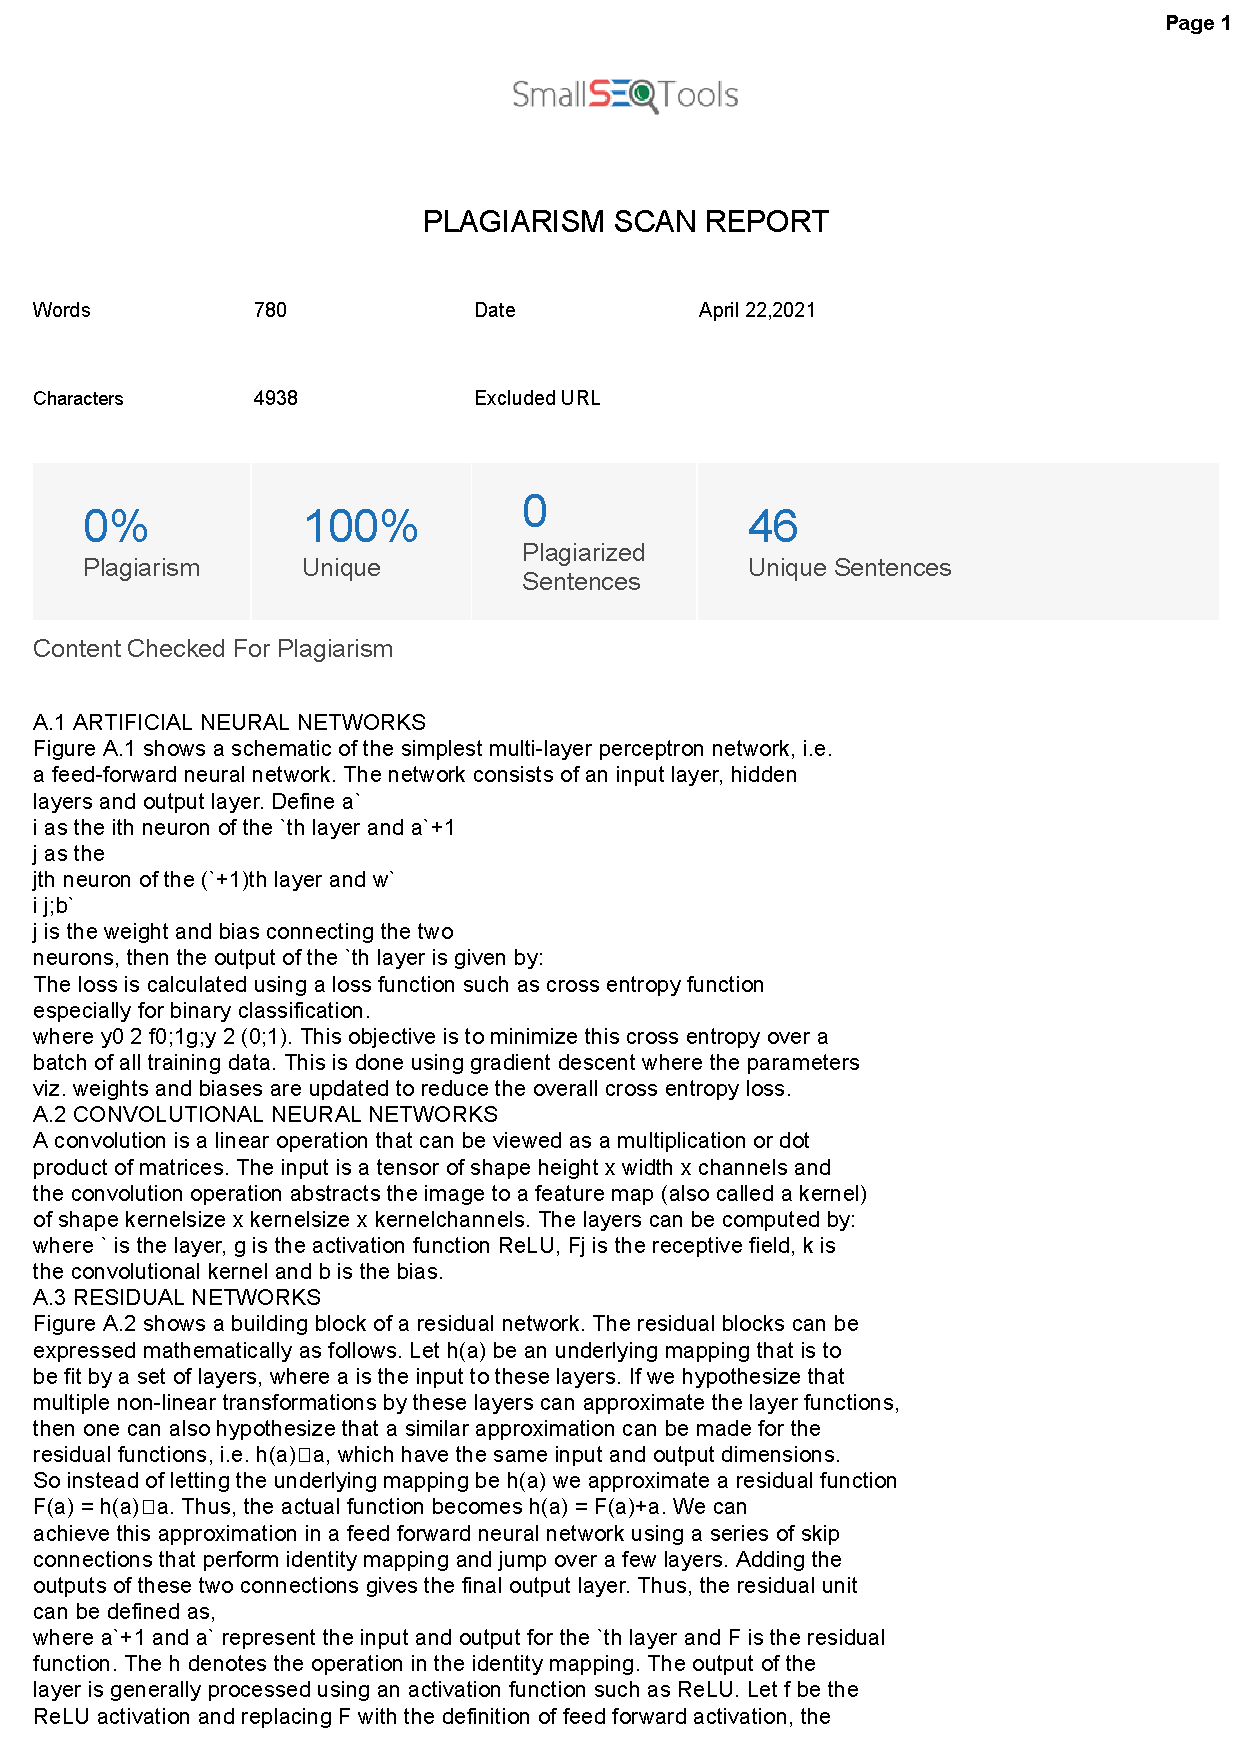
\includegraphics[scale=0.7, page=1]{plagiarism/mathematical_model.pdf}
    \end{subfigure}
 \caption{Plagiarism report for Mathematical Model}
    \label{PlagiarismMath}
\end{figure}
\begin{figure}\ContinuedFloat
    \begin{subfigure}[H]{\textwidth}
    	\centering
    	\includegraphics[scale=0.7, page=2]{plagiarism/mathematical_model.pdf}
    \end{subfigure}
    \caption{Plagiarism report for Mathematical Model (contd.)}
    \label{PlagiarismMath_1}
\end{figure}

\begin{figure}
	\begin{subfigure}[H]{\textwidth}
		\centering
    	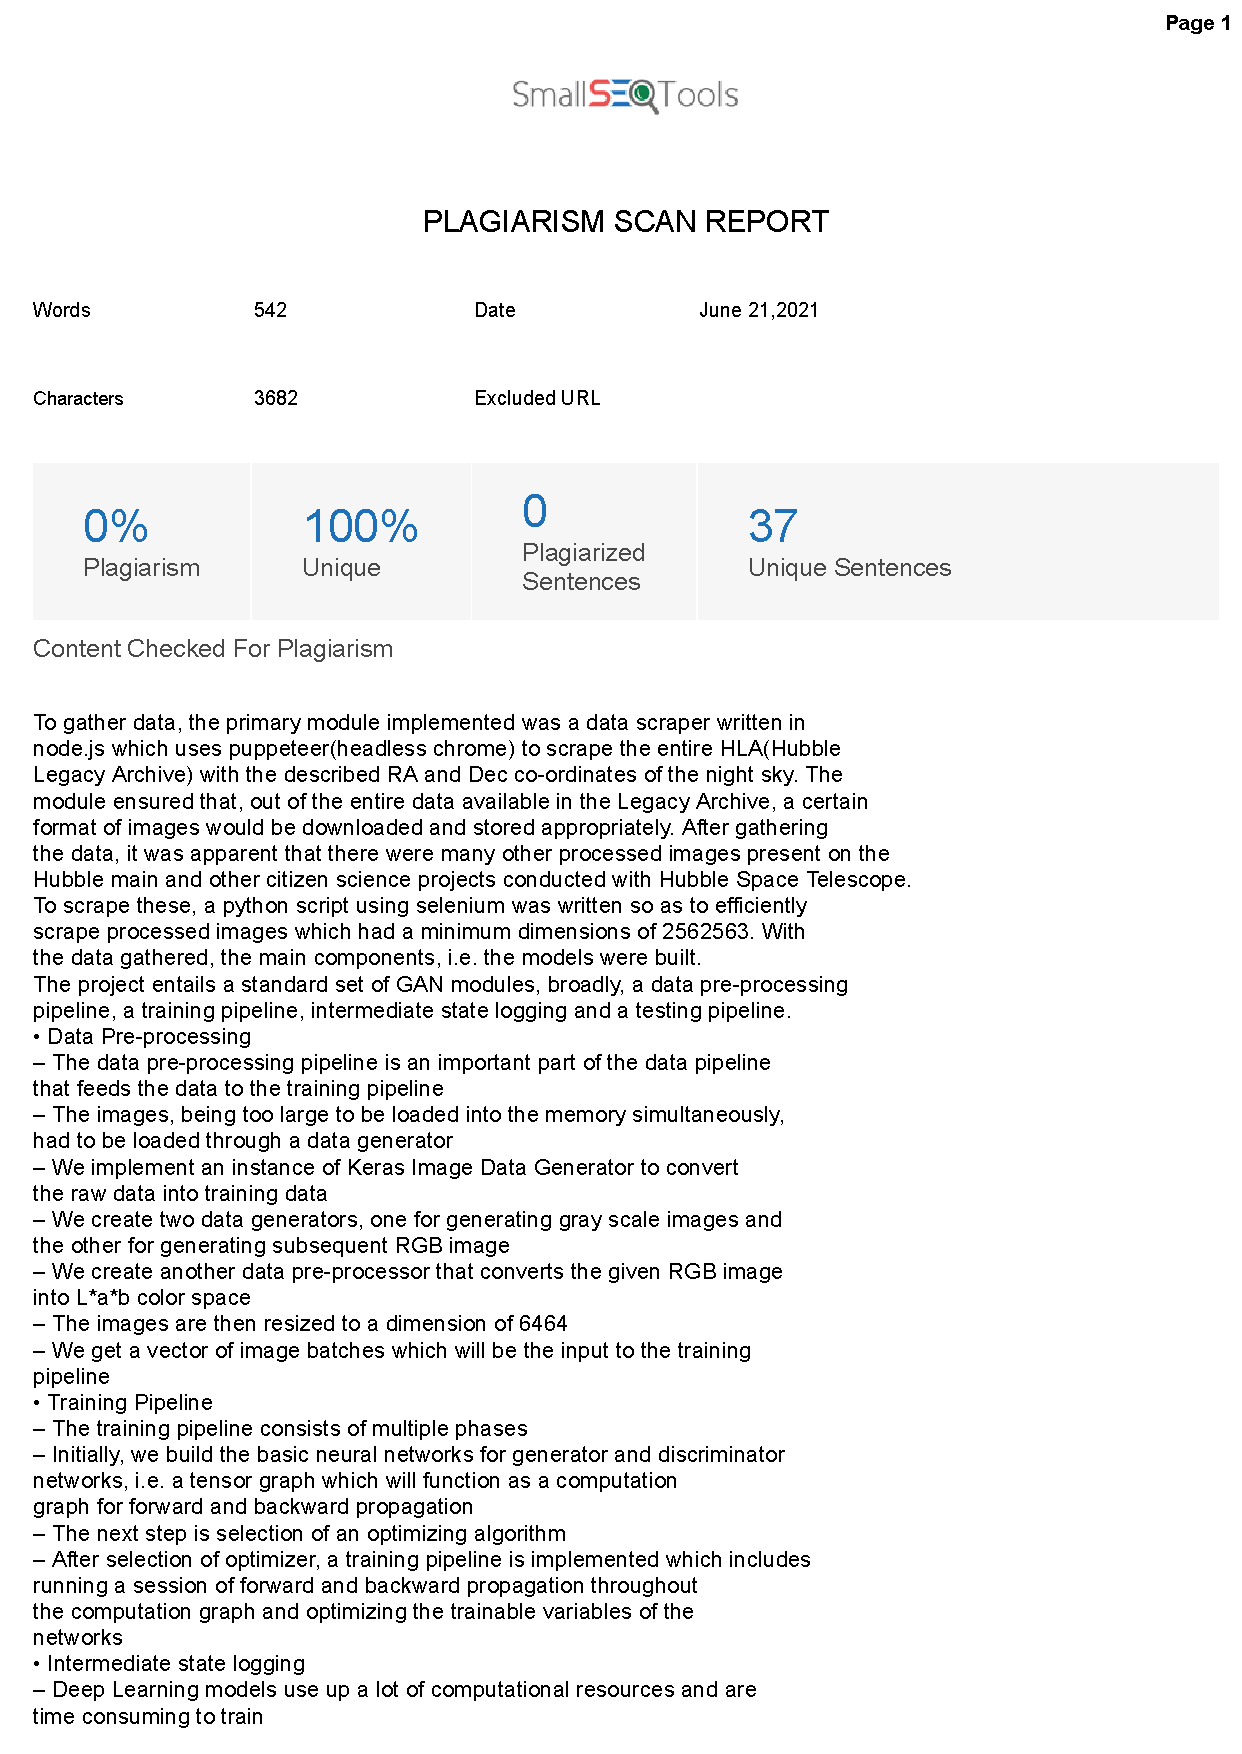
\includegraphics[scale=0.7, page=1]{plagiarism/project_implementation.pdf}
    \end{subfigure}
 \caption{Plagiarism report Project Implementation}
    \label{PlagiarismImplementation}
\end{figure}
\begin{figure}\ContinuedFloat
    \begin{subfigure}[H]{\textwidth}
    	\centering
    	\includegraphics[scale=0.7, page=2]{plagiarism/project_implementation.pdf}
    \end{subfigure}
    \caption{Plagiarism report for Project Implementation (contd.)}
    \label{PlagiarismImplementation_1}
\end{figure}

\begin{figure}
	\centering
    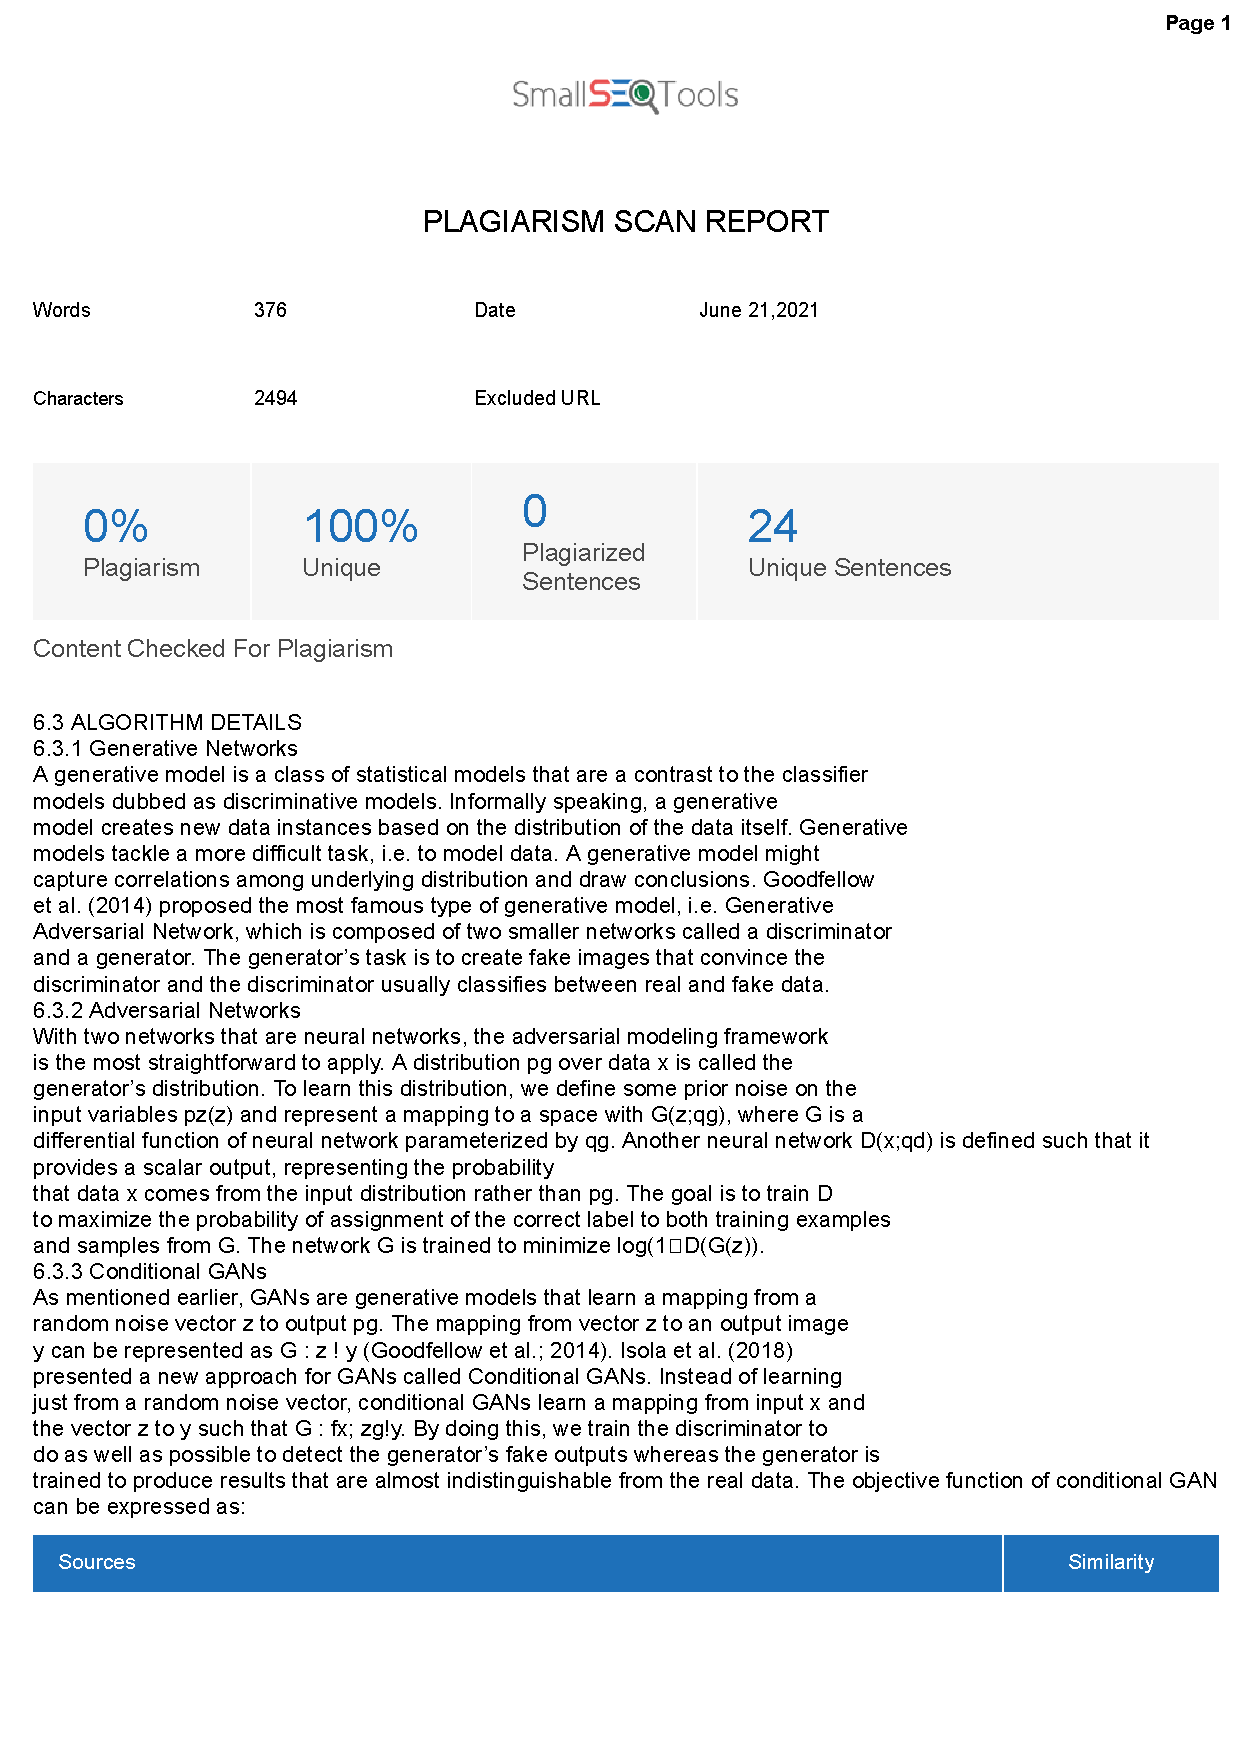
\includegraphics[scale=0.7]{plagiarism/algorithm_details.pdf}
    \caption{Plagiarism report for Algorithm Details}
    \label{PlagiarismAlgorithms}
\end{figure}

\begin{figure}
	\begin{subfigure}[H]{\textwidth}
		\centering
    	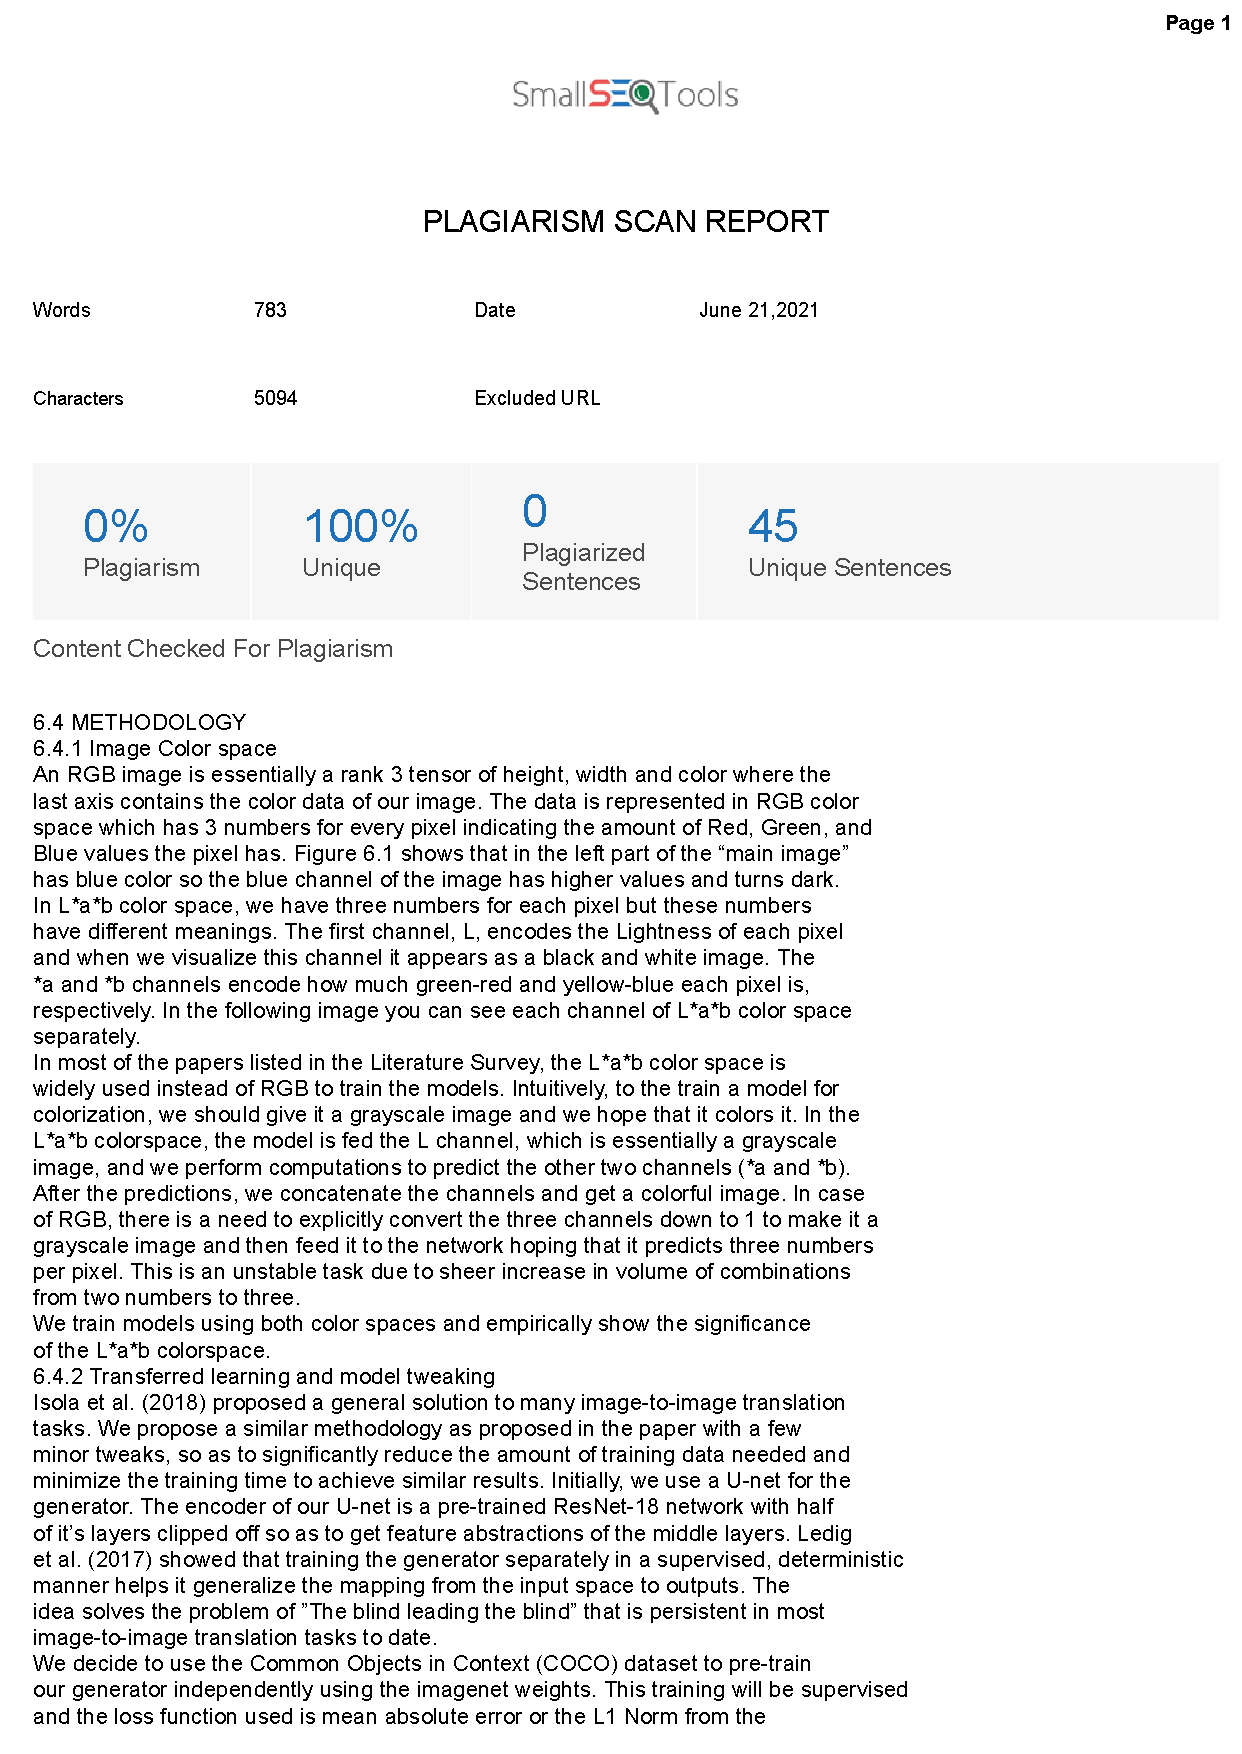
\includegraphics[scale=0.7, page=1]{plagiarism/methodology.pdf}
    \end{subfigure}
 \caption{Plagiarism report Methodology}
    \label{PlagiarismMethodology}
\end{figure}
\begin{figure}\ContinuedFloat
    \begin{subfigure}[H]{\textwidth}
    	\centering
    	\includegraphics[scale=0.7, page=2]{plagiarism/methodology.pdf}
    \end{subfigure}
    \caption{Plagiarism report for Methodology (contd.)}
    \label{PlagiarismMethodology_1}
\end{figure}

\begin{figure}
	\begin{subfigure}[H]{\textwidth}
		\centering
    	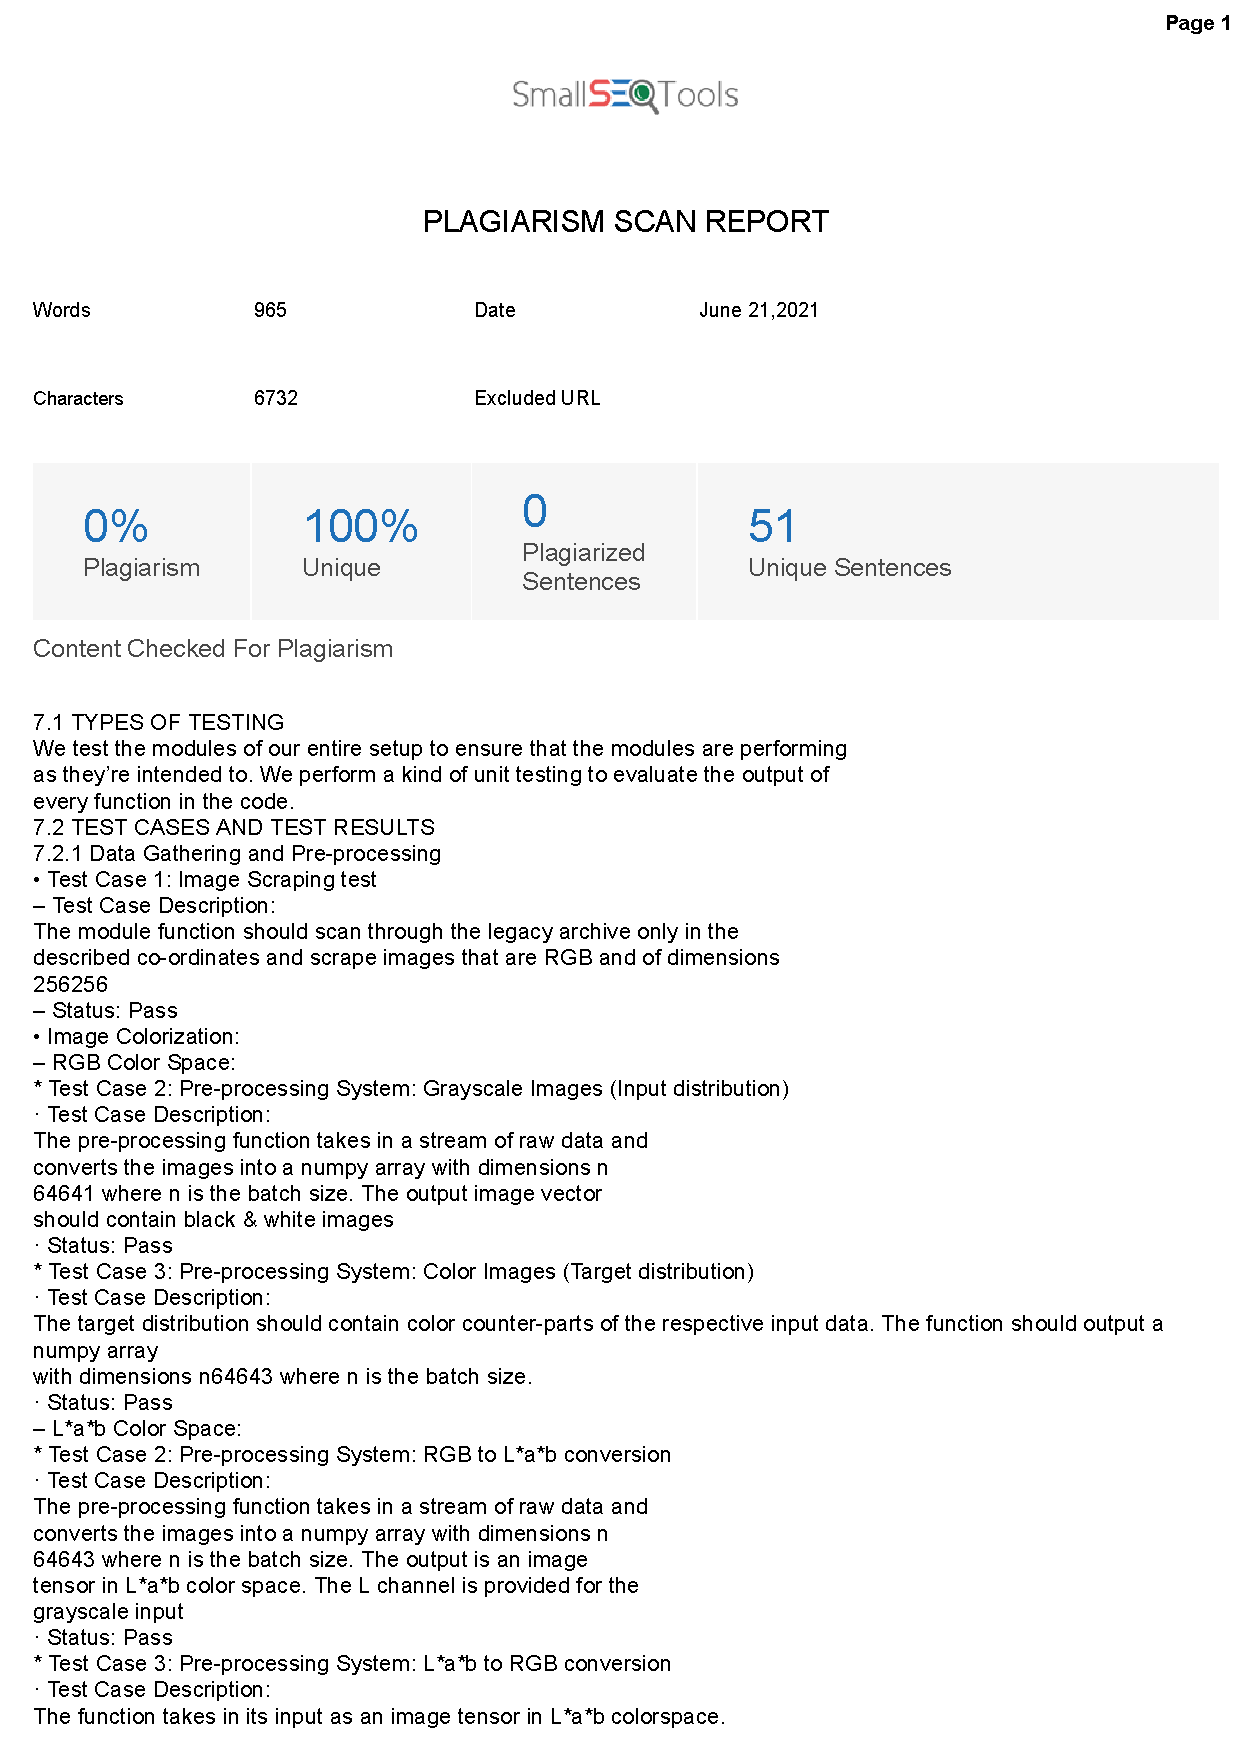
\includegraphics[scale=0.7, page=1]{plagiarism/software_testing.pdf}
    \end{subfigure}
 \caption{Plagiarism report Software Testing}
    \label{PlagiarismSoftwareTesting}
\end{figure}
\begin{figure}\ContinuedFloat
    \begin{subfigure}[H]{\textwidth}
    	\centering
    	\includegraphics[scale=0.7, page=2]{plagiarism/software_testing.pdf}
    \end{subfigure}
    \caption{Plagiarism report for Software Testing (contd.)}
    \label{PlagiarismSoftwareTesting_1}
\end{figure}
\begin{figure}\ContinuedFloat
    \begin{subfigure}[H]{\textwidth}
    	\centering
    	\includegraphics[scale=0.7, page=3]{plagiarism/software_testing.pdf}
    \end{subfigure}
    \caption{Plagiarism report for Software Testing (contd.)}
    \label{PlagiarismSoftwareTesting_2}
\end{figure}


\begin{figure}
	\centering
    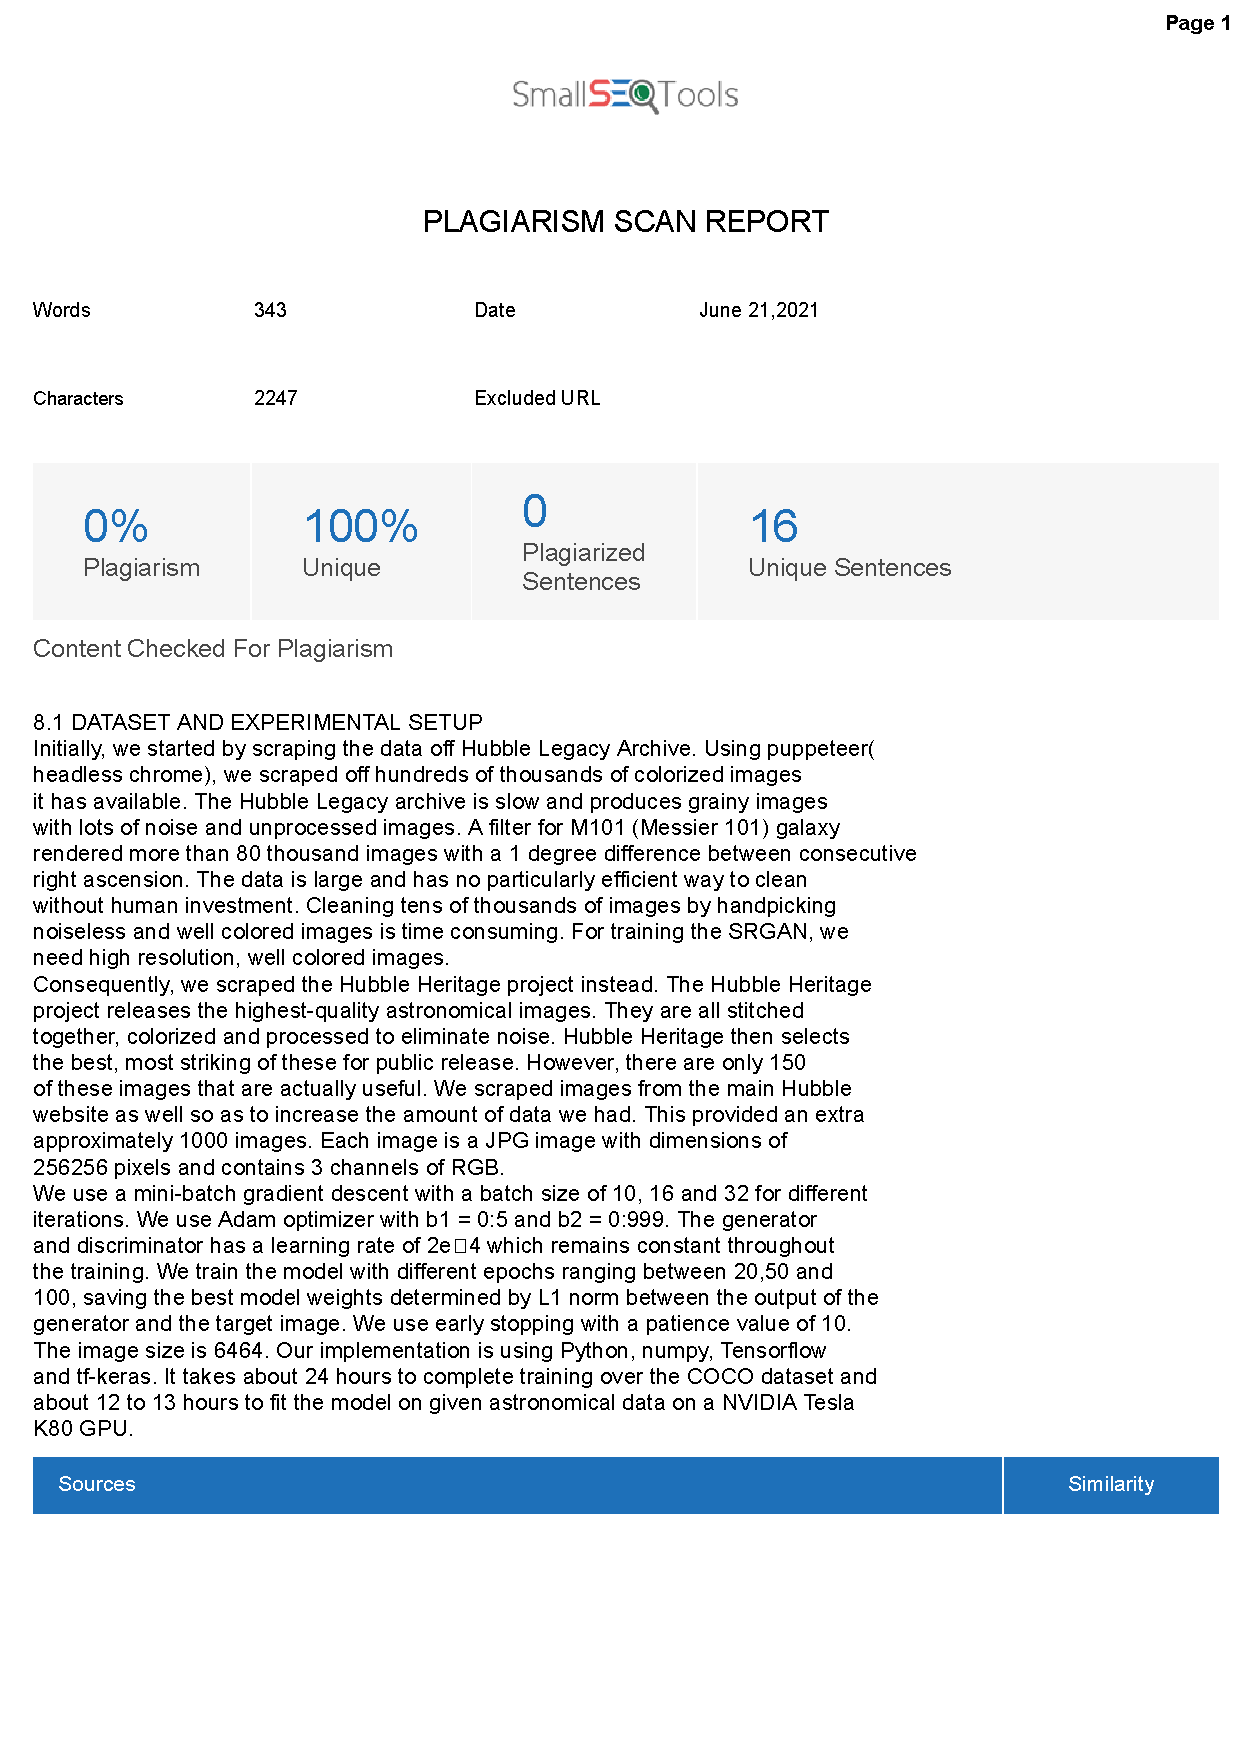
\includegraphics[width=\textwidth, height=\textheight]{plagiarism/dataset_experimental_setup.pdf}
    \caption{Plagiarism report for Experimental Setup}
    \label{PlagiarismExperiment}
\end{figure}

\begin{figure}
	\begin{subfigure}[H]{\textwidth}
		\centering
    	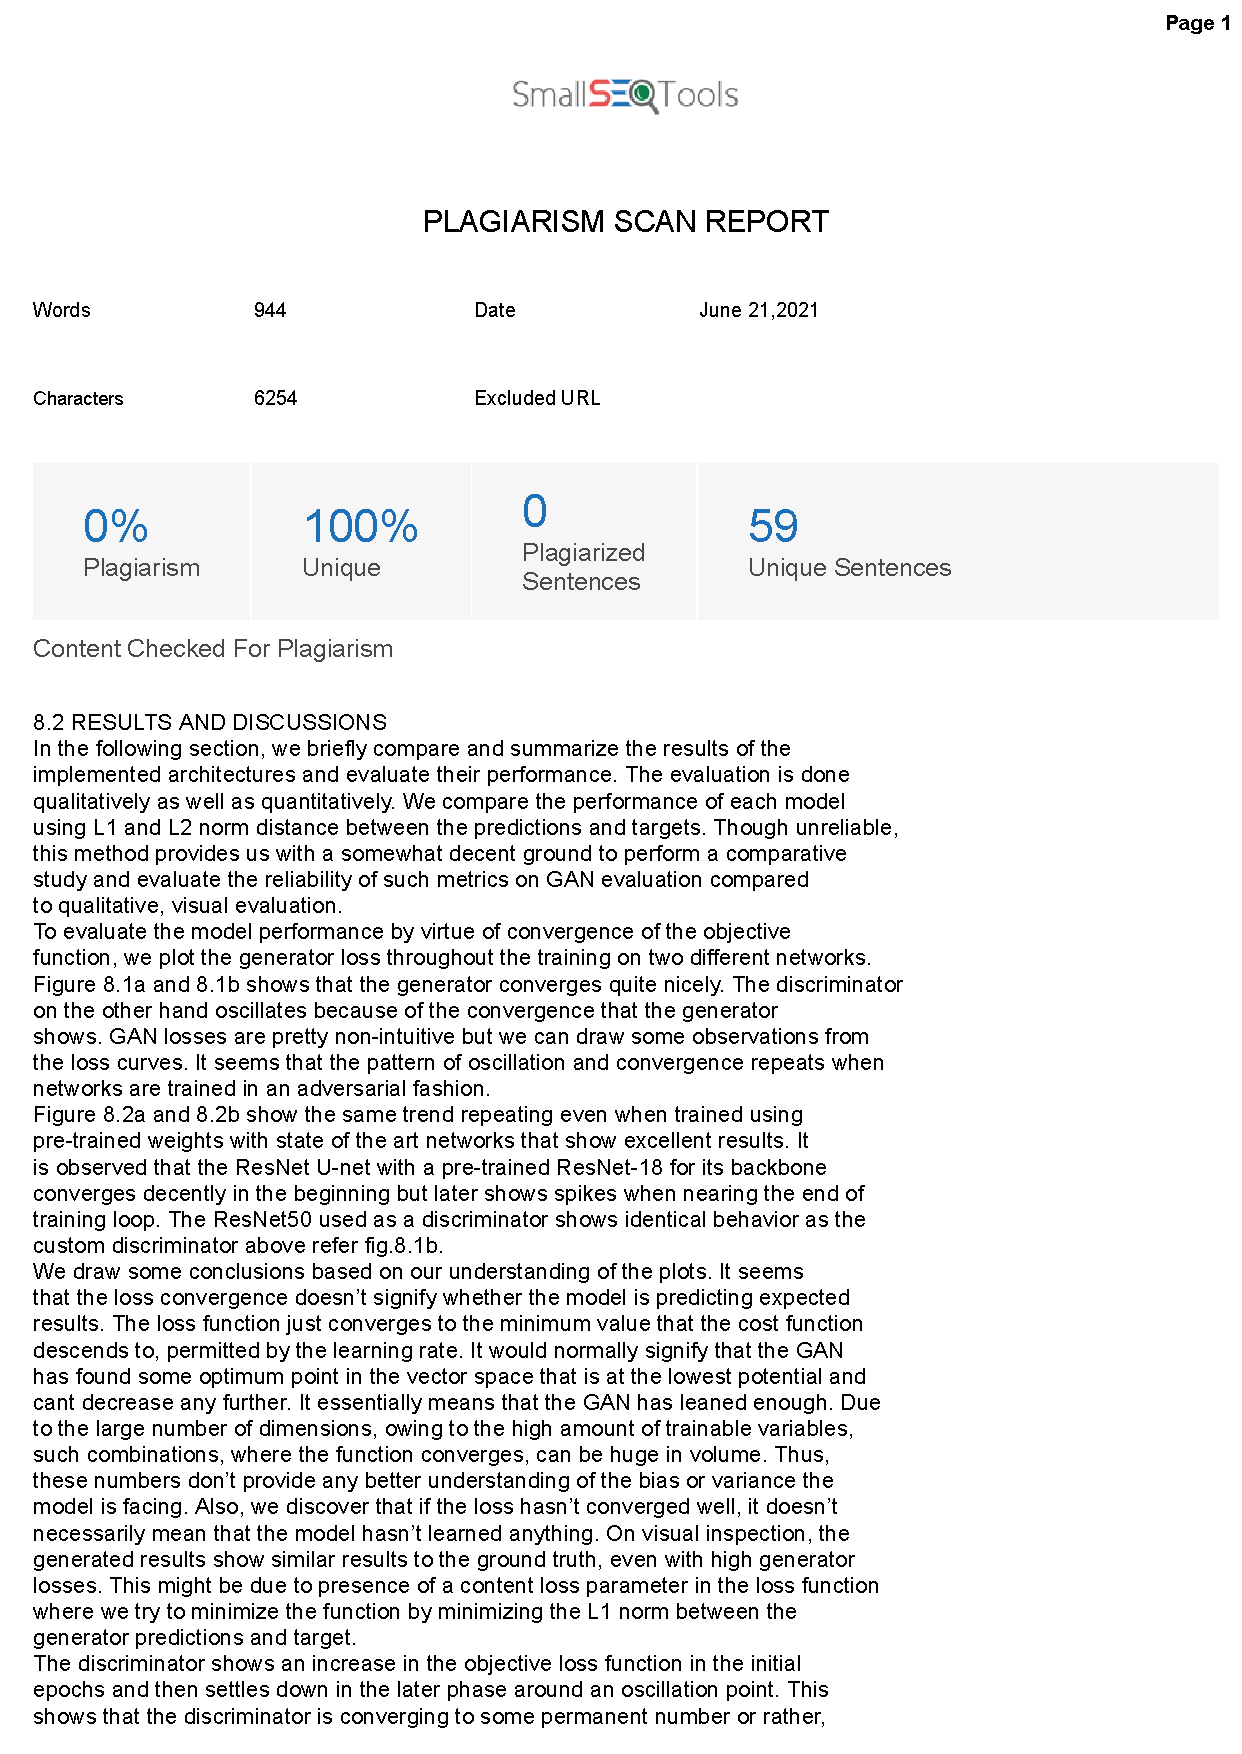
\includegraphics[scale=0.7, page=1]{plagiarism/results_1.pdf}
    \end{subfigure}
 \caption{Plagiarism report Results}
    \label{PlagiarismResults}
\end{figure}
\begin{figure}\ContinuedFloat
    \begin{subfigure}[H]{\textwidth}
    	\centering
    	\includegraphics[scale=0.7, page=2]{plagiarism/results_1.pdf}
    \end{subfigure}
    \caption{Plagiarism report for Results (contd.)}
    \label{PlagiarismResults_1}
\end{figure}
\begin{figure}\ContinuedFloat
    \begin{subfigure}[H]{\textwidth}
    	\centering
    	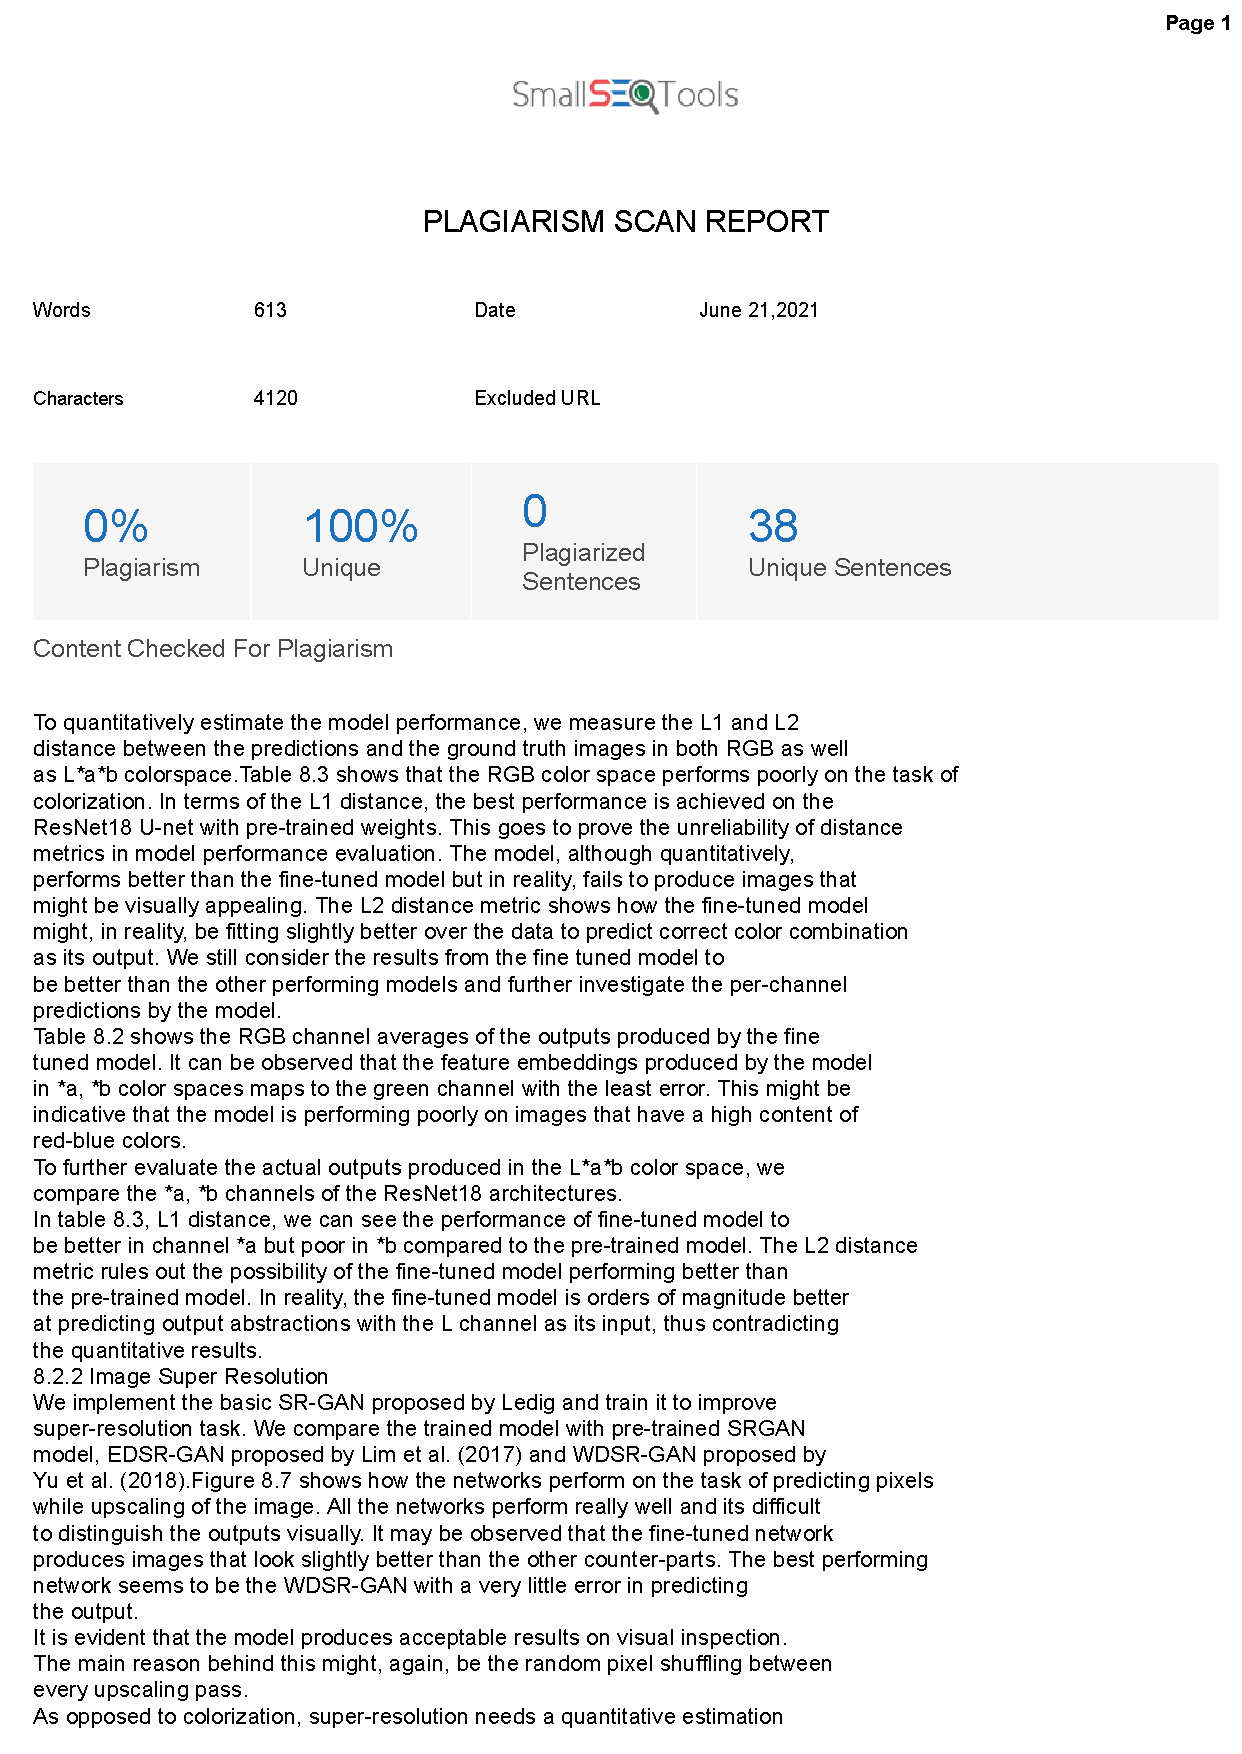
\includegraphics[scale=0.7, page=1]{plagiarism/results_2.pdf}
    \end{subfigure}
    \caption{Plagiarism report for Results (contd.)}
    \label{PlagiarismResults_2}
\end{figure}
\begin{figure}\ContinuedFloat
    \begin{subfigure}[H]{\textwidth}
    	\centering
    	\includegraphics[scale=0.7, page=2]{plagiarism/results_2.pdf}
    \end{subfigure}
    \caption{Plagiarism report for Results (contd.)}
    \label{PlagiarismResults_3}
\end{figure}

\begin{figure}
	\begin{subfigure}[H]{\textwidth}
		\centering
    	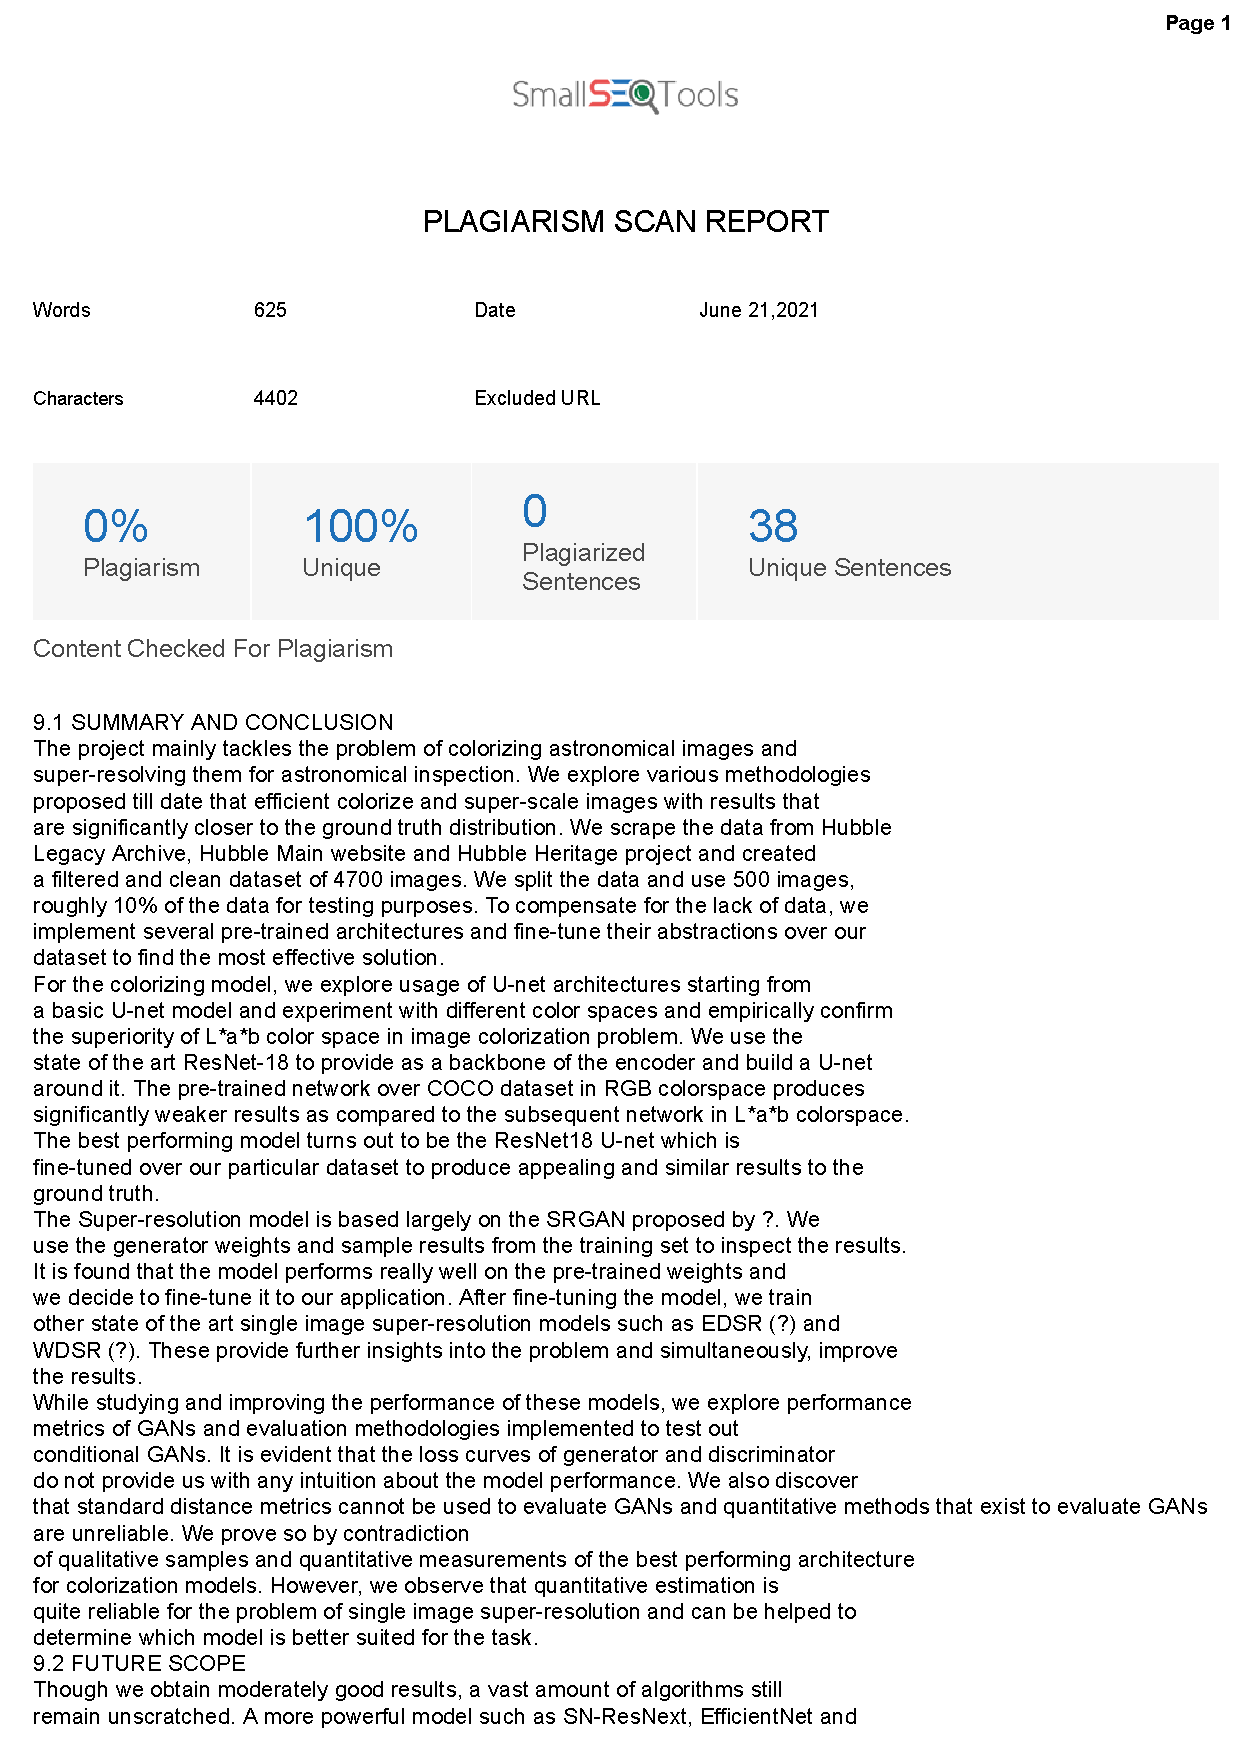
\includegraphics[scale=0.7, page=1]{plagiarism/summary_conclusion.pdf}
    \end{subfigure}
 \caption{Plagiarism report Summary and Conclusion}
    \label{PlagiarismSummary}
\end{figure}
\begin{figure}\ContinuedFloat
    \begin{subfigure}[H]{\textwidth}
    	\centering
    	\includegraphics[scale=0.7, page=2]{plagiarism/summary_conclusion.pdf}
    \end{subfigure}
    \caption{Plagiarism report for Summary and Conclusion (contd.)}
    \label{PlagiarismSummary_1}
\end{figure}

\end{appendices}


\end{document}
